\part{Estimating Dependency}
\label{partII}

\chapter{\acrlong{MCDE}}
\glsresetall
\label{chapter:MCDE}

The content of this chapter bases on the following publications: 

\begin{itemize}[noitemsep]
	\item \fullcite{DBLP:conf/ssdbm/FoucheB19}
	\item \fullcite{DBLP:conf/ssdbm/FoucheBMKB20}
\end{itemize}
\textbf{Keywords:} Multivariate Statistics; Exploratory Data Analysis; Dependency Estimation % Data Mining;  

\section{Chapter Overview} 

Estimating dependencies from data is a fundamental task of Knowledge Discovery. Identifying the relevant variables leads to a better understanding of data and improves both the runtime and the outcomes of downstream Data Mining tasks. 
Dependency estimation from static numerical data has received much attention.
However, real-world data often occurs as heterogeneous data streams. In this chapter, we make the following contributions:

\textbf{We present \gls{MCDE}}, a framework which satisfies both the constraints of heterogeneous data streams and the requirements of dependency estimation. Over a given time window, \gls{MCDE} estimates the dependency of an attribute set as the average discrepancy between marginal and conditional distributions, via Monte Carlo (MC) simulations. %In each MC simulation, MCDE applies a condition on each attribute. Then a statistical test quantifies the discrepancy between the marginal and conditional distributions. 
We determine a lower bound for the quality of our estimates, which only depends on the number of MC simulations. Such bound allows users to trade estimation accuracy for a computational advantage. 

\textbf{We explore three instantiations of \gls{MCDE}}, i.e., three new dependency measures, dubbed \gls{MWP}, \gls{KSP} and \gls{CSP}, which base on the corresponding statistical test. We show that using them in combination allows dealing with heterogeneous data. 
We describe their implementation and compare them to the existing multivariate methods in our experiments. 

\textbf{We introduce index structures} for \gls{MWP}, \gls{KSP}, and \gls{CSP}, to speed up contrast estimation. Our indexes support insertion/deletion operations for efficient estimation in streaming settings, e.g., over a sliding window.

\glsunset{Bioliq}
\textbf{We feature a use case against real-world data} from \gls{Bioliq} (cf. Section \ref{sec:bioliqexample}) and show how one can leverage \gls{MCDE} to discover interesting and useful patterns. We release our source code and experiments on GitHub\footnote{\url{https://github.com/edouardfouche/MCDE-experiments}}\textsuperscript{,}\footnote{\url{https://github.com/edouardfouche/MCDE-extended}}, with documentation to ensure reproducibility.

\section{Theory of \acrshort{MCDE}}

Dependency estimation determines to which extent a relationship differs from randomness. In this spirit, \gls{MCDE} quantifies dependence, i.e., a degree of independence violation, based on marginal and conditional distributions. Section \ref{sec:mcdenotations} introduced our notation. 

\subsection{Quantifying Dependency via Contrast}

A set of variables is \textit{independent} or \textit{uncorrelated} if and only if all variables are pairwise \textbf{mutually independent}. 
By treating the attributes of a subspace as random variables, we can define the independence assumption of a subspace: 
\begin{definition}[Independence Assumption]
	\label{IA1}
	The independence assumption $\mathcal{A}$ of a subspace $\gls{S}$  holds if and only if the random variables $\{ \gls{X_{s_i}} : \gls{s_i} \in \gls{S} \}$ are mutually independent, i.e.:
	\begin{equation}
	\mathcal{A}(\gls{S}) \Leftrightarrow \gls{p(X)} = \prod_{\gls{s_i} \in \gls{S}} \gls{p_{s_{i}}(X)} \label{eq:IA1}
	\end{equation}
\end{definition}
Under the independence assumption, the joint distribution of subspace $\gls{S}$ is \textbf{expected} to be equal to the product of its marginal distributions. We can define a degree of dependency %, or correlation, 
based on the degree to which $\mathcal{A}$ does not hold: 
\begin{definition}[Degree of Dependency]
	\label{DependencyDegree}
	The degree of dependency $\mathcal{D}$ of a subspace $\gls{S}$ is the discrepancy, abbreviated as `$disc$', between the \textbf{observed} joint distribution $p^{o}(\gls{X})$ and the \textbf{expected} joint distribution $p^{e}(\gls{X})$: 
	\begin{equation}
	\mathcal{D}(\gls{S}) \equiv disc \left(p^{o}(\gls{X}),p^{e}(\gls{X})\right) 
	\end{equation}
\end{definition} 
The discrepancy is a random variable. 
While one can estimate it between two probability distributions, using for instance the Kullback-Leibler divergence, %\cite{kullback1951information}
 this is not trivial here because $p^o(\gls{X})$ and $p^{e}(\gls{X})$ are a priori unknown. We work around this as follows: 
\begin{lemma}[Independence Assumption and Joint Distribution]
	\label{lemma1}
	The independence assumption $\mathcal{A}$ of subspace $\gls{S}$ states that the joint distribution for all  $S' \subset \gls{S}$  is equal to its conditional distribution on $\gls{S} \setminus S'$:
	\begin{equation}
	\mathcal{A}(\gls{S}) \Leftrightarrow p(X_{S'}|\overline{X_{S'}}) =  p(X_{S'}) \quad \forall S' \in \gls{P}(\gls{S})
	\end{equation}
\end{lemma} 
\begin{proof}[Proof of Lemma \ref{lemma1}]
	Since all variables in $\gls{S}$ are mutually independent, for any subspace $S' \in \gls{P}(\gls{S})$ we also have $p(X_{S'}) = \prod_{\gls{s_i} \in S'} \gls{p_{s_{i}}(X)}$:
	\begin{align*}
	\mathcal{A}(\gls{S}) &\Leftrightarrow~ \gls{p(X)} = \prod_{\gls{s_i} \in \gls{S}} \gls{p_{s_{i}}(X)} &&~ \\
	\mathcal{A}(S) &\Leftrightarrow~ \gls{p(X)} = p(X_{S'}) * \prod_{\gls{s_i} \in \gls{S} \setminus S'} \gls{p_{s_{i}}(X)} && \forall S' \in \gls{P}(\gls{S}) \\
	\mathcal{A}(\gls{S}) &\Leftrightarrow~ \frac{\gls{p(X)}}{p(\overline{X_{S'}})} = p(X_{S'}) && \forall S' \in \gls{P}(\gls{S})
	\intertext{By the definition of the conditional \textit{pdf}:}
	\mathcal{A}(\gls{S}) &\Leftrightarrow~ p(X_{S'}|\overline{X_{S'}}) =  p(X_{S'}) && \forall S' \in \gls{P}(\gls{S}) \label{lastofproof1} 
	\qedhere
	\end{align*}
\end{proof}

Lemma \ref{lemma1} provides an alternative definition of $\mathcal{A}$. However, it still has issues. % for the following reasons: 
First, multivariate density estimation is required to estimate $p(X_{S'})$ and $p(X_{S'}|\overline{X_{S'}})$ with $|S'| \geq 1$. 
Second, even if one could estimate $p(X_{S'})$ and $p(X_{S'}|\overline{X_{S'}})$, estimating the densities for all $ S' \in \gls{P}(\gls{S})$ is intractable. 
We instead relax the problem by considering only subspaces with  $|S'| = 1$, i.e., we only look at the marginal distribution of single variables. 
\begin{definition}[Relaxed Independence Assumption]
	The relaxed independence assumption $\mathcal{A}^*$ of a subspace $\gls{S}$ states that 
	the marginal distribution $\gls{p_{s_{i}}(X)}$ of each variable $\gls{s_i} \in \gls{S}$ equals $p_{s_{i}}(X|\overline{X_{s_i}})$, i.e., the conditional distribution of $\gls{s_i}$:
	\begin{align*}
	\mathcal{A}^*(\gls{S}) \Leftrightarrow p_{s_{i}}(\gls{X}|\overline{X_{s_i}}) = \gls{p_{s_{i}}(X)} \quad \forall \gls{s_i} \in \gls{S} 
	\end{align*}
\end{definition}

\begin{lemma}[Independence Assumption Relaxation] 
	\label{IA2}
	$\mathcal{A}(\gls{S}) \Rightarrow \mathcal{A}^*(\gls{S})$, i.e., we can relax $\mathcal{A}$ into $\mathcal{A}^*$ for any subspace $\gls{S}$.
\end{lemma}
\begin{proof}[Proof of Lemma \ref{IA2}]
	Using Lemma \ref{lemma1}:
	\begin{align*}
	\mathcal{A}(\gls{S}) &\Leftrightarrow p(X_{S'}|\overline{X_{S'}}) =  p(X_{S'}) && \forall S' \in \gls{P}(\gls{S}) \\
	\mathcal{A}(\gls{S}) &\Rightarrow p(X_{S^1}|\overline{X_{S^1}}) = p(X_{S^1}) && \forall S^1 \in \gls{P}(\gls{S}) :|S^1| = 1\\
	\mathcal{A}(\gls{S}) &\Rightarrow p_{s_i}(X|\overline{X_{s_i}}) = \gls{p_{s_{i}}(X)} && \forall \gls{s_i} \in \gls{S} 
	\qedhere
	\end{align*}
\end{proof}

Loosely speaking, the relaxed independence assumption holds if and only if the values of all variables but $\gls{s_i}$ do not reveal any information on $\gls{s_i}$. 
Next, $\mathcal{A}(\gls{S}) \Rightarrow \mathcal{A}^*(\gls{S})$, then $\neg \mathcal{A}^*(\gls{S}) \Rightarrow \neg \mathcal{A}(\gls{S})$, i.e., showing that $\mathcal{A}^*$ does not hold is sufficient but not necessary to show that $\mathcal{A}$ does not hold. 
Thus, we can define a relaxed degree of dependency $\mathcal{D}^*$ of a subspace $\gls{S}$, namely the discrepancy $disc$ of the observed marginal distribution $p^o_{s_i}(\gls{X})$ 
and the expected one $p^{e}_{s_i}(\gls{X})$. Under the relaxed independence assumption $\mathcal{A}^*$, we have $p^{e}_{s_i}(\gls{X}) = p^o_{s_i}(\gls{X}|\overline{X_{s_i}})$. 
We define $\mathcal{D}^*$ as the expected value $\mathbb{E}[.]$ of this discrepancy: 
\begin{definition}[Relaxed Degree of Dependency]
	\label{def:RelaxedDegree}
	\begin{equation}
	\mathcal{D}^*(\gls{S}) \equiv \mathop{\mathbb{E}}_{\gls{s_i} \in \gls{S}}   \Big[disc \left( p^o_{s_{i}}(\gls{X}) , p^o_{s_i}(\gls{X}|\overline{X_{s_i}}) \right)  \Big]
	\end{equation}
\end{definition}
This definition includes a whole class of dependency estimators, e.g., \cite{DBLP:conf/icde/KellerMB12}, which aim at quantifying the so-called  \textit{contrast} of a subspace. 
$\mathcal{D}^*$ -- or \textit{contrast} -- is a variant of $\mathcal{D}$ which is much easier to estimate. 
First, it relies on the comparison of marginal against conditional distributions, 
i.e., multivariate density estimation is not required. 
Second, the number of degrees of freedom of $\mathcal{A}^*(\gls{S})$ increases linearly with $|\gls{S}|$, but exponentially for $\mathcal{A}(\gls{S})$. Thus, estimating $\mathcal{D}^*$ instead of $\mathcal{D}$ allows coping with the strict efficiency requirements for data streams.  

By definition, $\mathcal{D}^*$ does not take the dependency between multivariate subsets into account, but only of each variable versus all others. 
However, we argue that this relaxation is not problematic, and it even supports interpretability.  
In fact, the detection of dependency is only interesting as long as we can observe effects w.r.t.\ the marginal and conditional distributions: in real-world scenarios, one is typically looking for interpretable influences of particular variables -- so-called targets -- on the system and vice versa \cite{DBLP:books/lib/HastieTF09}.

\subsection{Estimating Conditional Distributions}
\label{sec:slicing}

The difficulty when estimating $\mathcal{D}^*$ is estimating the conditional distributions, because the underlying data distributions are unknown. 
As proposed in \cite{DBLP:conf/icde/KellerMB12}, one can simulate conditional distributions by applying a set of conditions \mbox{to $\gls{S}$}, in a process called \textit{subspace slicing}. The concept of \textit{subspace slice} was defined so far only for numerical data. Here, we extend the definition of \textit{subspace slice} to handle heterogeneity by differentiating between numerical, ordinal and categorical attributes:  
\begin{definition}[Subspace Slice]
	\label{slice}
	A slice $c_{i}$ in a subspace $\gls{S}$ w.r.t. attribute $\gls{s_i}$ is a list of $\left |\gls{S} \right |-1$ conditions $C_j$ 
	 which restricts the values of each $s_j \in \gls{S} \setminus {\gls{s_i}}$: 
	\begin{equation*}
	\begin{split}
	c_i &= \left ( C_1, \dots, C_{i-1}, C_{i+1}, \dots, C_{|S|} \right ), \quad \text{where} \\
	C_j &= \begin{cases}
  \left[l_{j}, u_{j} \right]~s.t.~\left | \left \{\vec{\gls{x}}_k : x_{kj}  \in \left [l_{j}, u_{j} \right ] \right \} \right | = w' &\text{if}~ s_j \in \mathit{\gls{Num}}
\\ \left[l_{j} \dots u_{j} \right]~s.t.~\left | \left \{\vec{\gls{x}}_k : x_{kj}  \in \left [l_{j} \dots u_{j} \right ]\right \} \right | = w' &\text{if}~ s_j \in \mathit{\gls{Ord}}
\\ \left\{v_j: v_j \in s_j \right\}~s.t.~\left | \left \{\vec{\gls{x}}_k : x_{kj} \in \left\{v_j: v_j \in s_j \right\}  \right \} \right | = w' &\text{if}~ s_j \in \mathit{\gls{Cat}}
\end{cases} \\
&\forall j\in \{1, \dots, |\gls{S}|\} \setminus{i}
	\end{split} 
    \end{equation*} 
	where $\left[l_{j}, u_{j} \right]$ is a continuous interval,  $\left[l_{j} \dots u_{j} \right]$ is a discrete interval, and $\left\{v_j: v_j \in s_j \right\} $ is a set of values of $s_j$. $w' < \gls{w}$ is the number of observations per condition.  
	
	We call $\gls{s_i}$ the \textbf{reference} attribute, the only attribute without a condition.  
	We write that $\vec{\gls{x}}_k \in c_i$ if 
	$\vec{\gls{x}}_k$ fulfils all the conditions in $c_i$. We define $\overline{c}_i$ as the complementary slice, i.e., it contains all observations 
	which are not in $c_i$. 
	
	$p_{\gls{s_i} | c_i}(\gls{X})$ and $p_{\gls{s_i} | \overline{c}_i}(\gls{X})$ denote the conditional distribution of the observations in the slice $c_i$ and its complement $\overline{c}_i$, respectively.
$\mathcal{P}^{c}(\gls{S})$ is the set of all possible slices in subspace $\gls{S}$.
\end{definition}

We choose each condition in a slice independently at random, but so that they contain $w'$ observations. 
Note that ordinal and categorical attributes (e.g., gender) may have many tying values. In such a case, a random condition might not precisely have $w'$ elements. Our solution is to take a random condition containing at least $w'$ observations and randomly remove elements from the condition until only $w'$ observations remain.

We set $w' = \left \lceil \gls{w} \sqrt[|S|-1]{\alpha}\,  \right \rceil$ with $\alpha \in (0,1)$, so that, under the independence assumption, the expected share of observations in the slice equals $\alpha$. 
As a result, subspace slicing happens in a \textbf{di\-men\-sio\-na\-li\-ty-aware} fashion. 
When $\alpha$ is a constant, the expected number of observations per slice does not change with dimensionality. Thus, subspace slicing is a dynamic grid-based method based on the dimensionality of the subspace which alleviates to some extent the effects of the \textit{curse of dimensionality}.

Under the $\mathcal{A}^*$-assumption, the conditional distribution $p_{s_i|c_i}$ is equal to the marginal distribution $p_{s_i}$, for any attribute $\gls{s_i}$ and slice $c_i$. For brevity, we omit `$(\gls{X})$' in $\gls{p_{s_{i}}(X)}$ and  $p_{s_i|c_j}(\gls{X})$ in the following. 

\begin{lemma}[$\mathcal{A}^*$ and Conditional Distributions]
	\label{theorem2}
	\begin{align}
	\mathcal{A}^*(\gls{S}) \Leftrightarrow 
	p_{s_i | {c_i}} 
	&= 
	p_{s_i} 
	\quad \forall \gls{s_i} \in \gls{S},~\forall c_i \in \mathcal{P}^{c}(\gls{S}) 
	\end{align}
\end{lemma}

\begin{proof}[Proof of Lemma \ref{theorem2}]
By contradiction, using Lemma \ref{IA2}.
\begin{align*}
\intertext{`$\Leftarrow$': From  Lemma \ref{IA2}, assume $\mathcal{A}^*(\gls{S})$ and that } 
~& \exists s_j \in \gls{S} : p_{s_j}(\gls{X}|\overline{X_j}) \neq p_{s_j} \\
&\Rightarrow  \exists c_j \in \mathcal{P}^c(\gls{S}) : p_{s_j | c_j} \neq p_{s_j} \\
&\Rightarrow \text{Contradiction of Lemma \ref{theorem2}}  \notag
\intertext{`$\Rightarrow$': From Lemma \ref{theorem2}, assume $\mathcal{A}^*(\gls{S})$ and that }
~& \exists s_j \in S, \exists c_j \in \mathcal{P}^c(\gls{S}) : p_{s_j | c_j} \neq p_{s_j} \\
&\Rightarrow  p_{s_j}(\gls{X}|\overline{X_{s_j}}) \neq p_{s_j} \\
&\Rightarrow  \text{Contradiction of Lemma \ref{IA2}} \qedhere
\end{align*}
\end{proof}

\subsection{Discrepancy Estimation}

In reality, one only has a limited number of observations, i.e., one only has access to empirical distributions. 
A solution is to use a statistical test $\mathcal{T}$: 
\begin{align}
disc \left ( 
\hat{p}_{s_i} , \hat{p}_{s_i | {c_i}}
\right ) \equiv 
\mathcal{T}\left( \hat{p}_{s_i}, \hat{p}_{s_i | {c_i}} \right )
\end{align}
However, the number of observations is finite, and the observations that we use to estimate $\hat{p}_{s_i | {c_i}}$
are part of the ones used to estimate $\hat{p}_{s_i}$ so far. 
This is problematic, as statistical tests assume the samples to be distinct. Plus, when $\alpha \approx 1$, $\hat{p}_{s_i | {c_i}}$ converges to $\hat{p}_{s_i}$, i.e., the two populations are nearly the same. 
Conversely, $\alpha \approx 0$ yields spurious effects, since the sample from $\hat{p}_{s_i | {c_i}}$ then is small. 
We solve the problem by observing that $p_{s_i | {c_i}}$ and $p_{s_i | {\overline{c}_i}}$, the conditional distribution from the complementary slice $\overline{c}_i$, are equal under $\mathcal{A}^*$.  

\begin{theorem}[$\mathcal{A}^*$ and Complementary Conditions] \label{theorem3}
	\begin{align}
	\mathcal{A}^*(\gls{S}) \Leftrightarrow p_{s_i | {\overline{c}_i}} &= p_{s_i | {c_i}}
	\quad \forall \gls{s_i} \in \gls{S},~\forall c_i \in \mathcal{P}^{c}(\gls{S}) 
	\end{align}
\end{theorem}
\begin{proof}[Proof of Theorem \ref{theorem3}]
	By contradiction, using Lemma \ref{theorem2}.
	\begin{align*}
	\intertext{`$\Leftarrow$': From  Lemma \ref{theorem2}, assume $\mathcal{A}^*(\gls{S})$ and that $\exists s_j \in \gls{S}, \exists c_j \in \mathcal{P}^c(\gls{S}) : p_{s_j | c_j} \neq p_{s_j} $.}
	\intertext{\quad Since $p_{s_j} = p_{s_j | c_j \cup \bar{c}_j}$, then $\exists s_j \in \gls{S}, \exists c_j \in \mathcal{P}^c(\gls{S}) : p_{s_j | c_j} \neq p_{s_j | c_j \cup \bar{c}_j}$}
	&\Rightarrow \exists s_j \in \gls{S}, \exists c_j \in \mathcal{P}^c(\gls{S}) : p_{s_j | c_j} \neq p_{s_j | \bar{c}_j} \\
	&\Rightarrow  \text{Contradiction of Theorem \ref{theorem3}.} \\
	\intertext{`$\Rightarrow$': From  Theorem \ref{theorem3}, assume $\mathcal{A}^*(\gls{S})$ and that $\exists s_j \in \gls{S}, \exists c_j \in \mathcal{P}^c(\gls{S}) : p_{s_j | c_j} \neq p_{s_j | \bar{c}_j}$} 
	&\Rightarrow \exists s_j \in \gls{S}, \exists c_j \in \mathcal{P}^c(\gls{S}) : p_{s_j | c_j \cup c_j} \neq p_{s_j | \bar{c}_j \cup c_j}. \\
	\intertext{\quad Since $c_j \cup c_j = c_j$ and $p_{s_j} = p_{s_j | \bar{c}_j \cup c_j}$, then $\exists s_j \in \gls{S}, \exists c_j \in \mathcal{P}^c(\gls{S}) : p_{s_j | c_j} \neq p_{s_j}$}
	&\Rightarrow \text{Contradiction of Lemma \ref{theorem2}.} \qedhere
	\end{align*}
\end{proof}

Hence, one can evaluate $\mathcal{A}^*$ by looking at the discrepancies between the conditional distribution and its complementary conditional distribution. 
When doing so, the samples obtained from both distributions are distinct. 

We define our dynamic slicing scheme based on a parameter $\alpha$, the expected share of observations in the slice $c_i$. Thus, the expected share of observations $\overline{\alpha}$ in $\overline{c}_i$ equals $1-\alpha$. 
As a result, we set $\alpha = 0.5$ so that $\overline{\alpha} = \alpha$. 
This choice is judicious for statistical testing, as samples of equal size lead to higher statistical stability, and we get rid of parameter 
$\alpha$. 

\begin{figure}
	\begin{subfigure}[Numerical]
			{\label{fig:slicing-numerical}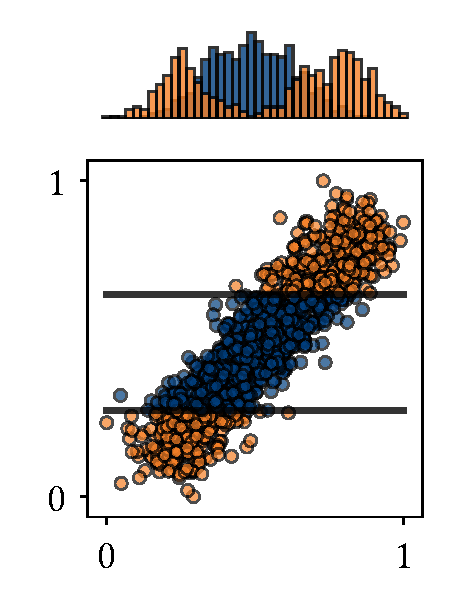
\includegraphics[width=0.241\textwidth]{part2-figures/mixed_1_2D_homo1-compressed.pdf}}
	\end{subfigure}
	\begin{subfigure}[Categorical]
			{\label{fig:slicing-categorical}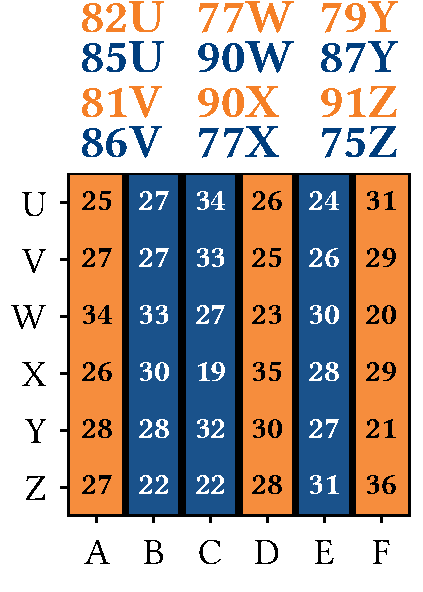
\includegraphics[width=0.241\textwidth]{part2-figures/mixed_0_2D_homo2-compressed-crop.pdf}}
	\end{subfigure} 
	\begin{subfigure}[Heterogeneous i.]
			{\label{fig:slicing-hetero1}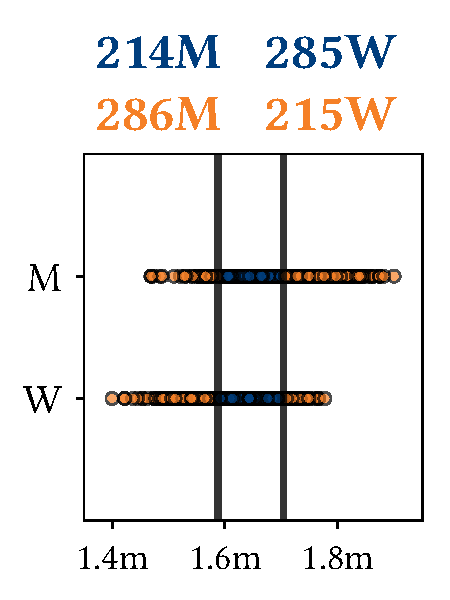
\includegraphics[width=0.241\textwidth]{part2-figures/mixed_0_2D_hetero1-compressed.pdf}}
	\end{subfigure}
	\begin{subfigure}[Heterogeneous ii.]
			{\label{fig:slicing-hetero2}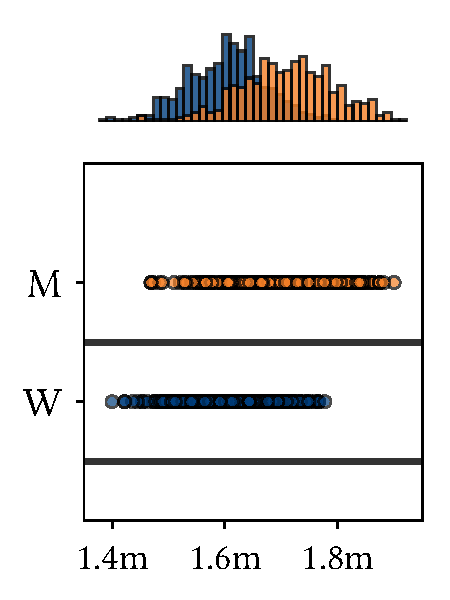
\includegraphics[width=0.241\textwidth]{part2-figures/mixed_1_2D_hetero2-compressed.pdf}}

	\end{subfigure} 
	\caption{Slicing in numerical, categorical, and heterogeneous subspaces ($|\gls{S}|=2$).} 
	\label{fig:slicing}
\end{figure} 

We illustrate slicing in heterogeneous subspaces in Figure \ref{fig:slicing}, with an exemplary numerical and categorical subspace in the left half and a heterogeneous subspace in the right half. 
The black lines show a random slice. The points in dark blue are in $c_i$, and the points in light orange are in $\overline{c}_i$. 
Figure \ref{fig:slicing-numerical} represents a numerical linear dependency. We can see from the histograms that, after slicing, the distribution of the points in each sample are very different. 
Figure \ref{fig:slicing-categorical} depicts the absolute frequencies of observing various symptoms $\{U \dots Z\}$ in different groups of patients $\{A \dots F\}$. 
Since there is no ordering within symptoms and patient groups, slicing in this case consists in selecting categories at random, here $\{B, C, E\}$. By comparing the absolute frequencies after slicing, we can determine whether there is a statistical association between groups and symptoms. 
Naturally, the statistical test that we use to estimate the discrepancy between $p_{s_i | {\overline{c}_i}}$ and $p_{s_i | {c_i}}$ might differ depending on the type of the reference attribute, as we will discuss later.  %This illustrate the major difference between slicing in a numerical or categorical space. 

Different attribute types can also be part of the same subspace, as we show in Figure \ref{fig:slicing-hetero1} and \ref{fig:slicing-hetero2}. We graph the height from a sample of individuals of two sexes. 
When we slice on the $x$-axis, the slice is a numerical interval. 
On the $y$-axis in turn, the slice is a category drawn at random. 

Intuitively, ordinal attributes share features from both numerical and categorical attributes: there exists an ordering between values, but typically also many tying values. In this case, we recommend using a similar slicing methodology as for numerical attributes, by selecting a discrete interval (see Definition \ref{slice}), and a statistical test that is robust to tying values to some extent. 

\subsection{Properties of Contrast}
\label{contrastproperties}

A statistical test $\mathcal{T}\left( B_1, B_2 \right)$ for two samples $B_1$ and $B_2$ typically yields a $p$-value. 
Traditionally, one uses $p$-values to assess the \textit{statistical significance}. %It is the probability to falsely reject a true null hypothesis, where the null hypothesis is the independence. 
Conversely, $\overline{p} = 1-p$ is known as \textit{confidence level}. % or probability to truly reject a false null hypothesis. 
The rationale behind estimating the degree of dependency $\mathcal{D}^*$ is to yield values quantifying the independence violation. 
We define \textit{contrast}, abbreviated as $\mathcal{C}$, as the expected value of the \textit{confidence level} of a statistical test $\mathcal{T}$ between the samples from the conditional distributions for all the possible attributes $\gls{s_i}$ and slices $c_i$:
\begin{definition}[Contrast $\mathcal{C}$]
	\label{def:contrast-test}
	\begin{align} 
	\mathcal{C}(\gls{S}) &\equiv
	\mathop{\mathbb{E}}_{c_i \in \mathcal{P}^{c}(\gls{S})}
	\Big [ \mathcal{T} \left (B(c_i), B(\overline{c}_i) \right ) \Big ]
	\end{align} 
	where $\mathcal{T}$ yields $\overline{p}$-values, and $B(c_i), B(\overline{c}_i)$ are the samples resulting from slicing. We draw the conditions in $c_i$ randomly and independently, w.r.t. any reference attribute $\gls{s_i}$ in subspace $\gls{S}$.
\end{definition}
By definition, %and independently from the underlying test,
$\mathcal{T} \sim \mathcal{U}[0,1]$ when the two samples are independent, and $\mathcal{T} \approx 1$ as the evidence against independence increases. The properties of $\mathcal{C}$ follow:
\begin{enumerate}[noitemsep]
	\item $\mathcal{C}$ converges to $1$ as the dependency in $\gls{S}$ increases.%, since the $p^c$-values converge to $1$ stochastically.
	\item $\mathcal{C}$ converges to $0.5$ when $\gls{S}$ is independent, since $\mathcal{T} \sim \mathcal{U}[0,1]$. %the distribution of the $p^c$-values converges to  $\mathcal{U}[0,1]$.
	\item $\mathcal{C}$ is bounded between $0$ and $1$.
\end{enumerate}
\label{mcde-properties}

\subsection{Monte Carlo Approximation}
\label{montecarlosimulation}
It is impossible to compute $\mathcal{C}$ exactly; one would need to know the distribution of $B(c_i)$ and $B(\overline{c}_i)$ 
for every slice. Instead, we approximate $\mathcal{C}$ via Monte Carlo (MC) simulations, with $M$ iterations. In each iteration, we choose the reference attribute $s_i$ and slice $c_i$ at random.  
We define the \textit{approximated contrast} $\mathcal{\widehat{C}}$:  

\begin{definition}[Approximated Contrast $\mathcal{\widehat{C}}$]
	\label{def:contrast-approx}
	\begin{align} 
	\mathcal{\widehat{C}}(\gls{S}) &= 
	\frac{1}{M} \sum_{m=1}^{M} \left [ \mathcal{T} \left(B\left(c_{i}  \right), B\left(\overline{c}_i\right)\right)~:~c_{i}  \overset{m}{\sim} \mathcal{P}^c(\gls{S}) \right ]
	\end{align} 
	where $c_{i} \overset{m}{\sim} \mathcal{P}^c(\gls{S})$ means that we draw $c_i$ randomly from $\mathcal{P}^c(\gls{S})$ in iteration~$m$.
\end{definition}

\label{bound} Interestingly, we can bound the quality of the approximation. From Hoeffding's inequality \cite{doi:10.1080/01621459.1963.10500830},
we derive a bound on the probability of $\mathcal{\widehat{C}}$ to deviate not less than $\varepsilon$ from $\mathcal{C}$. The bound decreases exponentially with increasing $M$:

\begin{theorem}[Hoeffding's Bound of $\mathcal{\widehat{C}}$]
	\label{"th:hoeffding-chernoff-contrast"}
	\begin{align}
	\Pr\left[| \mathcal{\widehat{C}} - \mathcal{C} | \geq \varepsilon \right] \leq 2e^{-2M \varepsilon^2}
	\end{align}
	where $M$ is the number of MC iterations, and $0 < \varepsilon < 1 - \mathcal{C}$. 
\end{theorem} 

\begin{proof}[Proof of Theorem \ref{"th:hoeffding-chernoff-contrast"}]
	Let us first restate Theorem 1 from \cite{doi:10.1080/01621459.1963.10500830} (see also Lemma \ref{hoeffdinginequality}): 
	Let $X_1, X_2, \dots, X_n$ be independent random variables $0 \leq X_i \leq 1$ for $i=1,\dots,n$ and let $\bar{X} = \frac{1}{n}(X_1 + X_2 + \dots + X_n)$ be their mean with expected value $E[\bar{X}]$. Then, for $0<t<1-E[\bar{X}]$, it holds that $\Pr[\bar{X}-E[\bar{X}] \geq t] \leq \e^{-2nt^2}$ and $\Pr[\bar{X}-E[\bar{X}] \leq t] \leq \e^{-2nt^2}$.

	We can treat each MC iteration $m_1, \dots, m_M$ as i.i.d. random variables $X_{m_1}, \dots, X_{m_M}$ with $0 \leq X_{m_i} \leq 1$. $\mathcal{\hat{C}}$ is the mean of the iterations with $E[\mathcal{\hat{C}}] = \mathcal{C}$ (\mbox{Definition \ref{def:contrast-test}}). Thus, for $0 < \varepsilon < 1 - \mathcal{C}$ it holds that
	\begin{align}
	\Pr[\mathcal{\hat{C}}-\mathcal{C} \geq \varepsilon] \leq \e^{-2M\varepsilon^2} && \Pr[\mathcal{\hat{C}}-\mathcal{C} \leq \varepsilon] \leq \e^{-2M\varepsilon^2}
	\end{align}
	since $\Pr[|\mathcal{\hat{C}}-\mathcal{C}| \geq \varepsilon] = \Pr[\mathcal{\hat{C}}+\mathcal{C} \geq \varepsilon] + \Pr[\mathcal{\hat{C}}-\mathcal{C} \geq \varepsilon]$ it is easy to verify Theorem~\ref{"th:hoeffding-chernoff-contrast"}.
\end{proof}

This is very useful. For instance, when $M=200$, the probability of $\mathcal{\widehat{C}}$ to deviate more than $0.1$ from its expected value is less than $2e^{-4} \approx 0.04$, and this bound decreases exponentially with $M$. Thus, one can adjust the computational requirements of $\mathcal{\widehat{C}}$ given the available resources, the desired quality level, or the rate of arrival of new observations in a stream. In other words, users can set $M$ intuitively, as it leads to an expected quality, and vice versa. Observe that $M$ is our only parameter. 

\subsection{Instantiating \gls{MCDE}}
\label{sec:instantiationMCDE}

One must instantiate $\mathcal{T}$ as a suitable statistical test. Ideally, $\mathcal{T}$ is non-parametric (\hyperlink{R4}{\textbf{R4}}) and suitable for the type of the reference attribute (numerical, ordinal, categorical). To facilitate meaningful experiments, we investigate instantiations  of \gls{MCDE}  based  on  three  well-known  non-parametric  tests: the Kolmogorov-Smirnov, the Mann-Whitney U and  the Chi-Squared test. We call the respective instantiations \gls{KSP}, \gls{MWP} and \gls{CSP}. 

The Kolmogorov-Smirnov test assumes the data to be continuous, i.e., it should be adequate for numerical attributes. 
The Mann-Whitney U test specifically handles tying values, so it might work well with ordinal attributes. 
Lastly, the Chi-Squared test bases on frequencies from a finite number of categories, i.e., we hypothesise it to be suitable for categorical attributes.
\begin{algorithm}\footnotesize
	\caption{\textsc{\gls{MCDE}}$(\gls{S} = \{s_1, \dots, s_{|\gls{S}|}\})$}\label{MCDE_alg}
	\begin{algorithmic}[1]
		\State $\mathcal{I} \gets$ \textsc{ConstructIndex}{$\left(\gls{S}\right)$} ; $\textit{result} \gets 0$ \label{MCDE_alg:line1}
		\For{$m \gets 1$ to $M$}
		\State $r \gets$ random integer in $\left[ 1,|\gls{S}| \right]$ 
		\State $slice \gets$ \textsc{Slice}{$\left(\mathcal{I}, r \right)$} \label{MCDE_alg:line4}
		\State $\textit{result} \gets \textit{result } +$ \textsc{Test}{$\left( \mathcal{I} , slice, r \right)$} \label{MCDE_alg:line5}
		\EndFor
		\State {\bfseries return} $(\textit{result} / M) \in (0,1)$
	\end{algorithmic}
\end{algorithm}

Algorithm \ref{MCDE_alg} summarises the general idea behind \gls{MCDE} for any arbitrary subspace $\gls{S} = \{s_1, \dots, s_{|\gls{S}|}\}$ of dimensionality $|\gls{S}|$. 
In practice, we can significantly improve the efficiency of slicing operations, which require the values of each attribute to be ordered, with an index structure (Line \ref{MCDE_alg:line1}). Afterwards, for $M$ iterations, we slice the data (Line~\ref{MCDE_alg:line4}) and carry out the statistical test (Line \ref{MCDE_alg:line5}). %We can do this efficiently thanks to the index, because tuples are sorted. 
The final estimate is the average of the test outcomes over $M$ iterations. In what follows, we present the specifics of the procedures \textsc{ConstructIndex}, \textsc{Slice} and \textsc{Test} for each instantiation of \gls{MCDE}. 

\section{Instantiation as \acrfull{MWP}}

We first consider the instantiation of $\mathcal{T}$ as a two-sided Mann-Whitney U test \cite{Mann1947}. %, as in our previous work \cite{DBLP:conf/kdd/FoucheKB19}. 
An advantage of this test is that it does not assume the data to be continuous, as it operates on ranks. So it is robust and applicable to numeric and ordinal measurements.  

\subsection{Estimating The Mann-Whitney U Statistics} 

In a nutshell, the Mann-Whitney U test compares the difference between the median of two samples. We review the definition of this test \cite{Siegel1956} between two samples $B_1$ and $B_2$ with size $n_1$ and $n_2$, and $n_1 + n_2 = \gls{w}$. It tests the null hypothesis that it is equally likely that a randomly selected value from one sample will be less than or greater than a randomly selected value from the other sample. $R_1$ and $R_2$ are the sums of ranks of the objects in $B_1$ and $B_2$, obtained by ranking the values of $B_1$ and $B_2$ together, starting with $0$. In case of ties, the ranks of the tying objects are \textit{adjusted}, i.e., become the average of their ranks. 
\begin{align}
p = \Phi(Z)~\text{or}~1-\Phi(Z) && Z = \frac{ U_i - \mu }{\sigma} && U_i = R_i - \frac{n_i(n_i-1)}{2}
\end{align}
Here, one can choose $U_i = U_1$ or  $U_i = U_2$ equivalently. $\Phi$ is the cumulative distribution function of the normal distribution, and $\mu$, $\sigma$ are defined as: 
\begin{align}
\mu = \frac{n_1 n_2}{2} && \sigma = \sqrt{\frac{n_1 n_2}{12} \left ( (\gls{w}+1) - \sum_{i=1}^{k} \frac{t_i^3 - t_i}{\gls{w}(\gls{w}-1)} \right ) }
\end{align}
The summation term of $\sigma$ is a correction for ties, where $t_i$ is the number of observations sharing rank $i$, and $k$ is the number of distinct ranks.
Typically, for $\gls{w} > 20$, the values of $U$ are normally distributed \cite{Mann1947} with mean $\mu$ and standard deviation $\sigma$. $Z$ is the standardised score, since \mbox{$Z \sim \mathcal{N}(0,1)$}. If $U = U_1$, then $Z \ll 0$ and $p \approx 0$ when the ranks of $A_1$ are stochastically smaller than those of $A_2$. Conversely, when the ranks of $A_1$ are stochastically larger, then $Z \gg 0$ and $p \approx 1$.
Both cases indicate an independence violation. As both directions are relevant, our test should capture them equally: %That is why we use the two-sided variant of the U test: 
\begin{align}
\text{MWP} = \Phi^{1/2}(Z') && Z' = |Z| && U = U_1
\end{align}
Since $Z  \sim \mathcal{N}(0,1)$, $Z'$ follows the so-called half-normal distribution with \textit{cdf} $\Phi^{1/2}$. Since $|U_1 - \mu|$ = $|U_2 - \mu|$, we can simply set $U = U_1$ or $U = U_2$ arbitrarily.%, i.e., one only needs to sum the ranks of one of the samples.

However, the ability of this test to detect dependency --  the `power' -- declines in the case of unequal variance of the two samples \cite{zimmerman2003warning, fagerland2009wilcoxon}. %This effect becomes problematic in case of unequal variance between marginal and conditional distributions. 
Thus, we include an additional step into the slicing process. 
It restricts the domain of the reference attribute $\gls{s_i}$ to a share $\alpha$ of observations. Formally, we define the marginal restriction as follows: 

\begin{definition}[Marginal Restriction]
	A marginal restriction is a condition on the reference attribute $\gls{s_i}$, i.e., an interval $r_i:[l_{i}, u_{i}]$ or $r_i:[l_{i} \dots u_{i}]$, so that $|\{ \vec{\gls{x}}_j : x_{ji} \in r_i \} | = \left \lceil \alpha \cdot \gls{w} \right \rceil = \left \lceil w' \right \rceil$ and the subspace slice becomes $c_i \cup r_i$.
\end{definition}

\begin{figure}
	\centering
	\hfill
	\begin{subfigure}[without MR]
		{\label{fig:circle-nomarginal}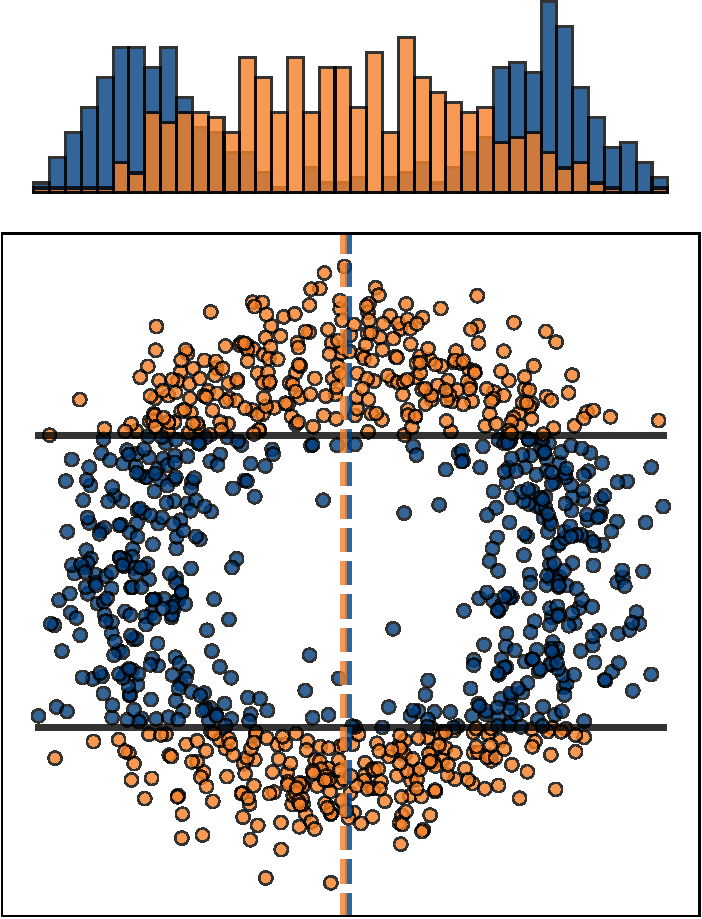
\includegraphics[width=0.21\textwidth]{part2-figures/circle_2D_0_nomarginal-crop-compressed.pdf}}
	\end{subfigure}
	\hfill
	\begin{subfigure}[with MR]
		{\label{fig:circle-marginal}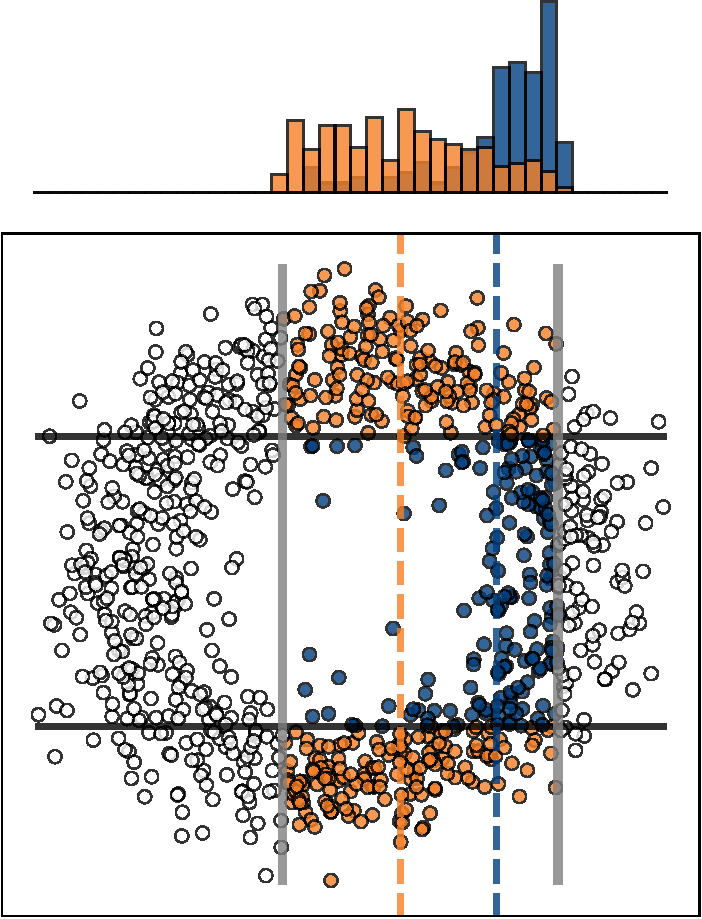
\includegraphics[width=0.21\textwidth]{part2-figures/circle_2D_0_marginal-crop-compressed.pdf}}
	\end{subfigure} 
	\hfill
	\begin{subfigure}[without MR]
		{\label{fig:linear-nomarginal}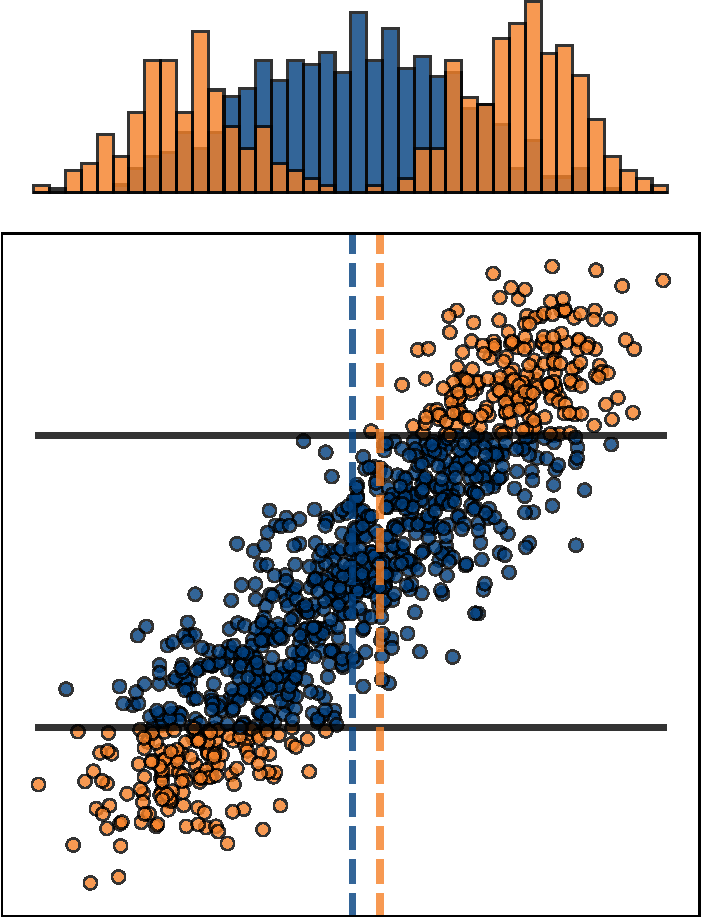
\includegraphics[width=0.21\textwidth]{part2-figures/linear_2D_0_nomarginal-crop-compressed.pdf}}
	\end{subfigure}
	\hfill
	\begin{subfigure}[with MR]
		{\label{fig:linear-marginal}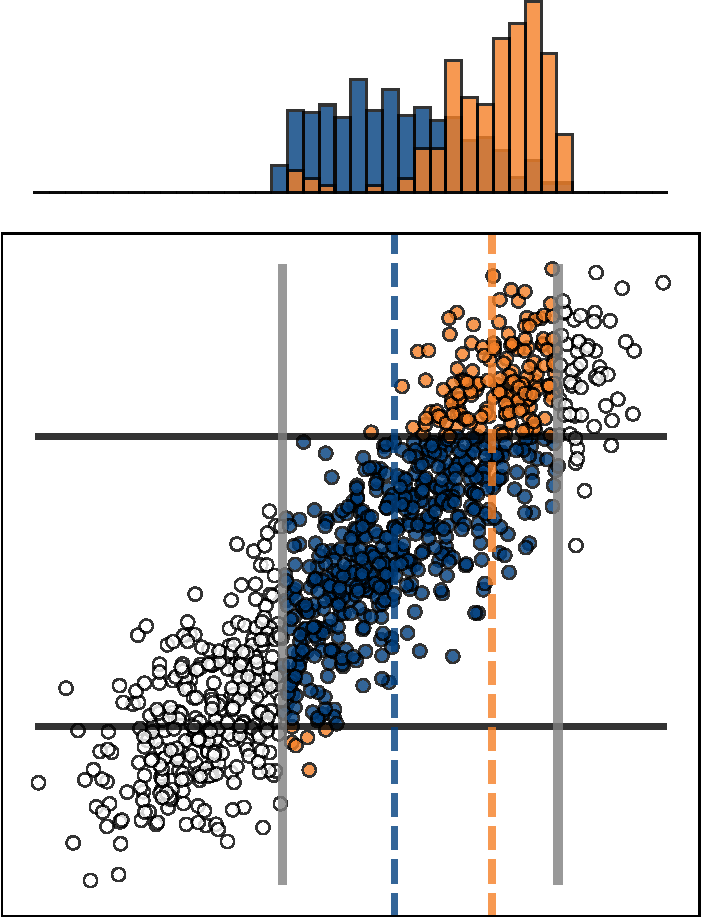
\includegraphics[width=0.21\textwidth]{part2-figures/linear_2D_0_marginal-crop-compressed.pdf}}
	\end{subfigure} 
	\hfill
	\caption{Marginal Restriction (MR) w.r.t. a circular and linear dependency ($|\gls{S}|=2$).} 
	\label{fig:slicing-marginal}
\end{figure}
We illustrate in Figure \ref{fig:slicing-marginal} the impact of the marginal restriction. 
We show in the left half a circular dependency and in the other half a linear dependency. 
Two grey lines show a marginal restriction (in \ref{fig:circle-marginal} and \ref{fig:linear-marginal}), and two vertical dashed lines stand for the median of each sample. 
%After slicing, both samples have highly unequal variance (see \ref{fig:circle-nomarginal} and \ref{fig:linear-nomarginal}). 
%However, in \ref{fig:circle-nomarginal}, the median of both distributions are nearly equal. Thus, this dependency remains undetected. 
We can see that in both cases, the marginal restriction leads to the median of the two samples having a larger difference. Thus, the discrepancy between both samples will be better detected by the Mann Whitney U test.
%The marginal restriction solves this problem, as we see in \ref{fig:circle-marginal}.  
%However, there is almost no difference between \ref{fig:linear-nomarginal} and \ref{fig:linear-marginal}. 
Intuitively, the marginal restriction `breaks the symmetry' between both distributions. 
Because of that, the MWP estimator with marginal restriction generally has higher statistical power.

\subsection{Implementation Details}
Algorithm \ref{indexconstruction} is the pseudo-code for the index construction. The index $\mathcal{I}$ is a 1-dimensional structure containing the adjusted ranks and tying value corrections for each attribute. It consists of $|\gls{S}|$ elements $\{I_1, \dots, I_{|\gls{S}|} \}$, where $I_i$ is an array of $4$-tuples sorted by $\gls{s_i}$ in ascending order.  
In this index, $l_i$ is the row numbers, $\tilde{x}_{i}$ are the sorted values
of $\gls{s_i}$, $a_i$ are the \textit{adjusted} ranks 
and $b_i$ the accumulated correction terms of the standard deviation $\sigma$.
$I_i[j]$ stands for the $j$-th tuple of $I_i$, and $l_{ji}$, $\tilde{x}_{ji}$, $a_{ji}$, $b_{ji}$ are its components.

Algorithm \ref{mwpslice} shows the slicing process. We can slice the input data efficiently because the tuples are already sorted in the index structure. 
We successively mask the row numbers based on a random condition for all but one reference attribute $s_r$. Additionally, we ensure that the condition boundaries do not split any tying values and that each condition has exactly $w'$ observations. 
The algorithm returns a $\mathit{slice}$, i.e., a list of $\gls{w}$ Boolean values, so we write $\mathit{slice} \in \mathbb{Z}_2^{\gls{w}}$. Since we visit each value at most once, the complexity is in  $O(|\gls{S}| \cdot\gls{w})$.

Algorithm \ref{TMWP} implements the statistical test based on our index. We determine a restriction $[\mathit{start}, \mathit{end}]$ on $s_{r}$ and sum the adjusted ranks of the observations in the slice. 
%Thanks to the marginal restriction, we compute the statistical test in a subsample of size $n' < n$. 
Since the ranks in this subset may not start from $0$, we adjust the sum of the ranks $R_1$ (Line \ref{adjustranks}). Then we compute a correction (Line \ref{corrects}) using the cumulative correction $b_r$ to adjust $\sigma$ for ties (Line \ref{tieshandling}). $\Phi^{1/2}$ is the cumulative distribution function of the half-Gaussian distribution.  
We compute the statistical test via a single pass, considering only elements between $\mathit{start}$ and $\mathit{end}$. Each operation requires constant time; The complexity is in $O(\gls{w})$.

\begin{algorithm}[ht]\footnotesize
	\caption{ \textsc{\gls{MWP}-ConstructIndex}$(\gls{S} = \{s_1, \dots, s_{|\gls{S}|}\})$}\label{indexconstruction}
	%\footnotesize
	\begin{algorithmic}[1]
		\For{$i = 1$ to $|\gls{S}|$} 
		
		\State $r_i \gets \left[0,\dots,\gls{w}-1\right]$
		\State $(l_i,\tilde{x}_i) \gets$ sort $(r_i, x_i)$ by $s_i$ in ascending order, break ties randomly
		\State $I_i \gets \left[(l_{1i}, \tilde{x}_{1i}, r_{1i}),\dots,(l_{wi}, \tilde{x}_{wi}, r_{wi})\right]$ %\COMMENT{Initialise $I_i:(l^i, r^i)$}
		\State $j \gets 1$ ; $\mathit{correction} \gets 0$
		\While{$j \leq \gls{w}$}
		\State $k \gets j$ ; $t \gets 1$ ; $\mathit{adjust} \gets 0$
		\While{$(k < \gls{w}-1) \wedge (s_{i}[l_{ki}] = s_{i}[l_{k+1,i}])$}
		\State $\mathit{adjust} \gets \mathit{adjust} + r_{ki}$ ; increment $k$ and $t$
		\EndWhile
		\If{$k > j$} %\COMMENT{Adjust the rank and correction}
		\State $\mathit{adjusted} \gets (\mathit{adjust} + r_{ki}) / t$ ; $\mathit{correction} \gets \mathit{correction} + t^3 - t$ 
		\State {\bfseries for} $m \gets j$ to $k$ {\bfseries do} $I_i[m] \gets (l_{mi}, \tilde{x}_{mi}, \mathit{adjusted}, \mathit{correction})$
		\EndIf
		\State {\bfseries else} $~~I_i[j] \gets (l_{ji}, \tilde{x}_{ji}, r_{ji}, \mathit{correction})$
		
		\State $j \gets j + t$
		\EndWhile
		
		\EndFor
		\State {\bfseries return} $\mathcal{I}: \{I_1, \dots, I_{|\gls{S}|} \}$ with $I_i: (l_i, \tilde{x}_i, a_i, b_i)$
	\end{algorithmic}
\end{algorithm}

\begin{algorithm}[ht]\footnotesize
	\caption{\textsc{\gls{MWP}-Slice}{$(\mathcal{I}: \{I_1, \dots, I_{|\gls{S}|} \}, r \in \{1,\dots,|\gls{S}|\})$}}\label{mwpslice} 
	\begin{algorithmic}[1]
		\State $w' \gets \left \lceil \gls{w} \cdot \sqrt[|\gls{S}|-1]{\alpha}\,  \right \rceil  $
		\For{$I_i \in \mathcal{I} \setminus I_{r}$} 
		\State $\mathit{slice}_i \gets$ Array of $\gls{w}$ Boolean values initialised to $\mathit{false}$
		\State $\mathit{start} \gets$ random integer in $[1,\gls{w}-w']$
		\State $\mathit{end} \gets$ $\mathit{start} + w'$
		\State {\bfseries while} $r_{\mathit{start},i} = r_{\mathit{start}-1,i}$ {\bfseries do} $\mathit{start} = \mathit{start} -1$
		\State {\bfseries while} $r_{\mathit{end},i} = r_{\mathit{end}+1,i}$ {\bfseries do} $\mathit{end} = \mathit{end} + 1$
		\State {\bfseries for} $j \gets \mathit{start}$ to $\mathit{end}$  {\bfseries do} $\mathit{slice}[l_{ji}] \gets \mathit{true}$
		
		\If{$\mathit{end} - \mathit{start} > w'$}
		\State $nb \gets \mathit{end} - \mathit{start} - w'$
		\State $\mathit{exclude} \gets$ draw $nb$ sample from $[\mathit{start}, \mathit{end}]$ without replacement
		\State {\bfseries for} $el \in \mathit{exclude}$ {\bfseries do} $\mathit{slice}[el] \gets \mathit{false}$
		\EndIf
		
		\EndFor
		\State $\mathit{slice}_r \gets$ Array of $\gls{w}$ Boolean values initialised to $\mathit{true}$
		\State $\mathit{slice} \gets \mathit{slice}_1 \wedge \dots \wedge \mathit{slice}_{|\gls{S}|}$
		\State {\bfseries return} $\mathit{slice} \in \mathbb{Z}_2^{\gls{w}}$
	\end{algorithmic}
\end{algorithm}

\begin{algorithm}[ht]\footnotesize
	\caption{\textsc{\gls{MWP}-Test}{$( \mathcal{I}: \{I_1, \dots, I_{|\gls{S}|} \}, \mathit{slice} \in \mathbb{Z}_2^{\gls{w}}, r \in \{1,\dots,|\gls{S}|\})$}}\label{TMWP}
	%\footnotesize
	\begin{algorithmic}[1]
		\State $\mathit{start} \gets$ random integer in $[1,\gls{w} \cdot (1-\alpha)]$ 
		\State $\mathit{end} \gets$ $\mathit{start} + \left \lceil \gls{w} \cdot \alpha \right \rceil$
		
		\State $R_1 \gets 0$ ; $n_1 \gets 0$
		\For{$j \gets \mathit{start}$ to $\mathit{end}$} 
		\If{$\mathit{slice}[l_{jr}] = \mathit{true}$}
		\State $R_1 \gets R_1 + a_{jr}$ 
		\State $n_1 \gets n_1 + 1$
		\EndIf
		\EndFor
		\State{$w' \gets \mathit{end} - \mathit{start} $} %
		\State {\bfseries if} $n_1 = 0$ or $n_1 = w'$ {\bfseries return} $1$
		\State $U_1 \gets R_1 - \mathit{start} \cdot n_1$   \label{adjustranks}
		\State $n_2 \gets w' - n_1$
		\State $\mu \gets (n_1 \cdot n_2)/ 2$
		\State $\mathit{correction} \gets (b_{\mathit{end}-1,r}-b_{\mathit{start}-1,r})/(w'\cdot (w'-1))$ \label{corrects}
		\State $\sigma \gets \sqrt{((n_1 \cdot n_2)/12) \cdot {(w'+1-\mathit{correction})}}$ \label{tieshandling}
		\State {\bfseries return}  $\Phi^{1/2}(|U_1 - \mu| / \sigma) \in (0,1)$
	\end{algorithmic}
\end{algorithm}

\clearpage

\section{Instantiation as \acrfull{KSP}}
\label{sec:instantiatingKSP}

\subsection{Estimating Kolmogorov-Smirnov Statistic}

We now describe another instantiation of \gls{MCDE}, which uses the two-sample Kolmogorov-Smirnov (KS) test. 
The KS test is non-parametric, and it is widely used to test the equality of two continuous one-dimensional probability distributions. 
It is adequate in case the reference attribute is numerical. However, it is known that the KS test has less power in the presence of ties \cite{DBLP:books/daglib/0023683}. %p584
So it may not work well with ordinal attributes. 
% See the discussion from here: https://stats.stackexchange.com/questions/1047/is-kolmogorov-smirnov-test-valid-with-discrete-distributions

In a nutshell, the two-sample Kolmogorov-Smirnov statistic $D$ is the supremum of the absolute differences of the empirical cumulative distribution functions $F_{1}(x)$ and $F_{2}(x)$ of Samples $1$ and $2$ with $n_1$ and $n_2$ elements: 
\begin{equation}
    D = \sup_{x} \left | F_{1}(x) - F_{2}(x) \right |
\end{equation}
\gls{HiCS} employed this test statistic to quantify contrast. 
However, to comply with the \gls{MCDE} framework, one must first derive the corresponding $\overline{p}$-value. 
The $\overline{p}$-values are not trivial to obtain, because the distribution of $D$ does not have any known closed form, and the time required for an exact computation increases with $n_1$ and $n_2$ in particular.  
To obtain the $\overline{p}$-values, we approximate them using the asymptotic Kol\-mo\-go\-rov-Smir\-nov distribution proposed in \cite{durbin1973distribution}: 
\begin{equation}
\label{asymptotic-ks}
\Pr \left[D \sqrt{ \frac{n_1 \cdot n_2}{n_1+n_2}} \leq x\right] = 1 -2 \sum_{i=1}^{\infty} (-1)^{i -1} e^{-2i^2x^2}
\end{equation}
Empirically, we found that summing up the first $1000$ terms of the expansion provides enough accuracy, without much impact on the execution time. %EF: Alternatively, we could have a fixed tolerance 
Using this approximation is common practice within most modern statistical software, such as R \cite{R}. 

\subsection{Implementation Details}

%EF: We could also have used the java program from "Computing the Two-Sided Kolmogorov-Smirnov Distribution" (https://core.ac.uk/download/pdf/6287952.pdf)
%EF: The code from Alan somewhat correspond to the approximation that R does as well. The ks.test function use this approximation as long as n*m > 10000, (which is our case mostly). See the function pkstwo from ks.c. However, the difference is that they don't have a fixed number of iteration, but a fixed tolerance (which is maybe nicer?). They refer to J. Durbin (1973), Distribution Theory for Tests Based on the Sample Distribution Function.  SIAM.
%EF: The other method which I implemented is exact (as long as there is no tie), it copies methods psmirnov2x and what it does is explained here: https://r.789695.n4.nabble.com/ks-test-The-two-sample-two-sided-Kolmogorov-Smirnov-test-with-ties-PR-13848-td923859.html
%EF: Found also here: https://stat.ethz.ch/pipermail/r-devel/2009-July/054106.html
%EF: I wonder whether we need to detail both alternatives (the exact the approximate one). Ideally, it would be nicer to have the approximation with a fixed tolerance (say 1e-6 or even 1e-3).  
%EF: I appears that "Marsaglia's algorithm" is for the exact computation of the one-sample test. It is also implemented in ks.c. However, "Computing the Two-Sided Kolmogorov-Smirnov Distribution" (https://core.ac.uk/download/pdf/6287952.pdf) argue that it is slow. 
%EF: Find the ks.c source in the R sources at /src/library/stats/src/ks.c
%EF: Statsexchange discussion: https://stats.stackexchange.com/questions/149595/ks-test-how-is-the-p-value-calculated
%Optional: The importance to break ties arbitrarily?

Algorithm \ref{kspconstructindex} is the pseudo-code for the index construction. The difference to \gls{MWP} is that we do not need to adjust ranks or precompute tie correction, because the Kolmogorov-Smirnov test assumes that there are no tying values. 
The resulting data structure contains the indices $l_i$ and the values $x_i$ of each attribute $\gls{s_i}$, ordered by $\gls{s_i}$ in ascending order. 

\begin{algorithm}\footnotesize
	\caption{ \textsc{\gls{KSP}-ConstructIndex}$(\gls{S} = \{s_1, \dots, s_{|\gls{S}|}\})$}\label{kspconstructindex}
	%\footnotesize
	\begin{algorithmic}[1]
		\For{$i = 1$ to $|\gls{S}|$} 
		
		\State $r_i \gets \left[0,\dots,\gls{w}-1\right]$
		\State $(l_i,\tilde{x}_i) \gets$ sort $(r_i, x_i)$ by $\gls{s_i}$ in ascending order, break ties randomly
		\State $I_i \gets \left[(l_{1i}, \tilde{x}_{1i}),\dots,(l_{wi}, \tilde{x}_{wi})\right]$ 
		\EndFor
		\State {\bfseries return} $\mathcal{I}: \{I_1, \dots, I_{|\gls{S}|} \}$ with $I_i: (l_i, \tilde{x}_i)$
	\end{algorithmic}
\end{algorithm}

Similarly, Algorithm \ref{kspslicing} is responsible for slicing, but does not require any further step to handle ties. Algorithms \ref{indexconstruction} and \ref{kspconstructindex} as well as Algorithms \ref{mwpslice} and \ref{kspslicing} respectively behave in the same way whenever the data does not have ties. 

\begin{algorithm}\footnotesize
	\caption{\textsc{\gls{KSP}-Slice}{$(\mathcal{I}: \{I_1, \dots, I_{|\gls{S}|} \}, r \in \{1, \dots, |\gls{S}|\})$}}\label{kspslicing}
	%\footnotesize
	\begin{algorithmic}[1]
		\State $w' \gets \left \lceil \gls{w} \cdot \sqrt[|\gls{S}|-1]{\alpha}\,  \right \rceil  $
		\For{$I_i \in \mathcal{I} \setminus I_{r}$} 
		\State $\mathit{slice}_i \gets$ Array of $\gls{w}$ Boolean values initialised to $\mathit{false}$
		\State $\mathit{start} \gets$ random integer in $[1,\gls{w}-w']$
		\State $\mathit{end} \gets$ $\mathit{start} + w'$
		\State {\bfseries for} $j \gets \mathit{start}$ to $\mathit{end}$  {\bfseries do} $\mathit{slice}[l_{ji}] \gets \mathit{true}$
		\EndFor
		\State $\mathit{slice}_r \gets$ Array of $\gls{w}$ Boolean values initialised to $\mathit{true}$
		\State $\mathit{slice} \gets \mathit{slice}_1 \wedge \dots \wedge \mathit{slice}_{|\gls{S}|}$
		\State {\bfseries return} $\mathit{slice} \in \mathbb{Z}_2^{\gls{w}}$
	\end{algorithmic}
\end{algorithm}

Algorithm \ref{KSPtest} implements the KS test. We compute the statistic $D$, i.e., the largest difference of the two empirical cumulative distribution functions in Lines \ref{start-computing-D}--\ref{end-computing-D}. 
Then we approximate the $\overline{p}$-value with Equation \ref{asymptotic-ks} in Line \ref{ks-approx}. 

% Scala code to pseudecode notation
% ref.length: n
% indexSelection: slice 
% reference: r 
% inSlice: n1
% outSlice: n2
% selectIncrement: u 
% refIncrement: v
% acc1: Zeta_1 
% acc2: Zeta_2
% currentMax: D
% summation: Phi

\begin{algorithm}\footnotesize
    \caption{\textsc{\gls{KSP}-Test}{$( \mathcal{I}: \{I_1, \dots, I_{|\gls{S}|} \}, \mathit{slice} \in \mathbb{Z}_2^{\gls{w}}, r \in \{1,\dots,|\gls{S}|\} )$}}\label{KSPtest}
    \begin{algorithmic}[1]
        \State $n_1 \gets \left|\{ i: i \in [1\dots \gls{w}] \wedge \mathit{slice}[l_{ir}] = \textit{true} \}\right|$ % Nb of elements being $true$ in $slice$
        \State $n_2 \gets \gls{w} - n_1$ 

        \State {\bfseries if} $n_1 = 0$  {\bfseries or} $n_2 = 0$ {\bfseries return} $1$
        \State $u \gets 1/n_1$ ; $v \gets 1/n_2$
        \State $\zeta_1 \gets 0$ ; $\zeta_2 \gets 0$
        \State $D \gets 0 ; \phi \gets 0$ 
        \For{$i \gets 1$ to $\gls{w}$} \label{start-computing-D}
            \State {\bfseries if} $\mathit{slice}[l_{ir}] = true$ {\bfseries then} $\zeta_1 \gets \zeta_1 + u $
            \State {\bfseries else} $\zeta_2 \gets \zeta_2 + v $
            \State $D \gets max \{D, |\zeta_2 - \zeta_1| \}$
        \EndFor \label{end-computing-D}
        \State $z \gets D \sqrt{n_1 n_2 / (n_1 + n_2)}$
        \State {\bfseries for} $i \gets 1$ to $1000$ {\bfseries do} $\phi \gets \phi + (-1)^{i-1}e^{-2i^2z^2}$ \label{ks-approx}
        \Return $(1 - 2 \phi) \in (0,1)$
    \end{algorithmic}
\end{algorithm}

\section{Instantiation as \acrfull{CSP}}

\subsection{Estimating Chi-Squared Statistic}

The Chi-Squared test, also known as Pearson's Chi-Squared test, perhaps is the most famous non-parametric test. In short, it determines whether there is a significant difference between the expected frequencies and the observed frequencies of a set of categories. 

For a reference variable $\gls{s_i} \in \mathit{\gls{Cat}}$ with categories $A = \{a_1, \dots, a_{|A|}\}$, we sketch the contingency table w.r.t.\ the two samples $B(c_i)$ and $B(\overline{c}_i)$ in Table~\ref{tab:contingencytable}, where $o^i_j$ is the absolute frequency of Category $a_{j}$ in Sample $i$, and we have:
\begin{align}
    \sum_{i=1}^{|A|}{o^j_i} &= o^j && j \in \{1,2\} \\
\sum_{j=1}^{2}{o^j_i} &= o_i && i \in \{1, \dots, |A|\} 
\end{align}
\begin{table}
\caption{Exemplary Contingency Table.}
\label{tab:contingencytable}
\centering
\renewcommand{\arraystretch}{1.3}
\begin{tabular}{lccccc}
\toprule
                    & $a_1$ & $a_2$ & \dots & $a_{|A|}$      & Total \\
\midrule
Sample 1: $B(c_i)$         & $o^1_{1}$ & $o^1_{2}$ & \dots & $o^1_{{|A|}}$ & $o^1$ \\
Sample 2: $B(\overline{c}_i)$ & $o^2_{1}$ & $o^2_{2}$ & \dots & $o^2_{{|A|}}$ & $o^2$ \\
Total                       & $o_{1}$   & $o_{2}$   & \dots & $o_{{|A|}}$   & $\gls{w}$  \\
\bottomrule
\end{tabular}
\end{table}
Then we can compute the test statistic $Q$ as follows:
\begin{equation}
    Q = \sum_{i=1}^{|A|}\sum_{j=1}^{2} \frac{(o_i^j-e_i^j)^2}{e_i^j}
\end{equation}
where $e_i^j = o_i \cdot o^j / \gls{w}$ 
is the expected absolute frequency. 

Under independence, $Q$ follows the $\chi^2$ distribution with cumulative distribution function $\chi^2_k: \mathbb{R}^+ \mapsto [0,1]$, where $k = |A|-1$ is the number of degrees of freedom. Thus, $\chi^2_k(Q)$ leads to the $\overline{p}$-value that we use for \gls{CSP}. 

\subsection{Implementation Details}

As with the other instantiations, we improve the execution time with an index. It contains the position of each occurrence of a categorical value binned into its respective category. 
Algorithm \ref{cspconstructindex} is our pseudo-code for its construction. We can construct the index in linear time with a single pass over each attribute, as it does not require any sorting.

Algorithm \ref{cspslicing} is our slicing procedure for \gls{CSP}. The main difference to \gls{MWP} and \gls{KSP} is that the index is not ordered. Thus, slicing consists in selecting a random set of categories per attribute. The algorithm ensures that exactly $w'$ observations are part of each condition.

Finally, Algorithm \ref{CSPtest} shows how to compute the Chi-Squared statistic, based on the information from the index and a subspace slice. 

\subsection{Complexity}

The overall complexity of \gls{MWP} and \gls{KSP} is in $O(|\gls{S}| \cdot (\gls{w} \cdot log(\gls{w}) + \gls{w}) + M \cdot(|\gls{S}| \cdot \gls{w} + \gls{w}))$. Since $|\gls{S}| \ll \gls{w}$, this simplifies to $O(\gls{w} \cdot log(\gls{w}) + M\cdot \gls{w})$. The index construction is asymptotically the most expensive step, as it is in $O(\gls{w} \cdot log(\gls{w}))$. Since the index construction for CSP does not require sorting, this step simplifies to $O(\gls{w})$. 
However, one only needs to construct the index once for a given data set or window. When the index is available, one can compute the estimator in linear time for the exponential number of subspaces. 

Interestingly, \gls{MCDE} is trivial to parallelise: one can compute the elements of the index structure $I_1, \dots, I_{|\gls{S}|}$ in parallel, as they are independent of each other. Similarly, one can parallelise each Monte Carlo iteration. This is useful, as multi-core architectures are ubiquitous in modern database systems. 
Thus, \gls{MCDE} scales well with the size of the data set. We will verify this claim via experiments in Section \ref{sec:scalability}.

\begin{algorithm}\footnotesize
	\caption{ \textsc{\gls{CSP}-ConstructIndex}$(\gls{S} = \{s_1, \dots, s_{|\gls{S}|}\})$}\label{cspconstructindex}
	%\footnotesize
	\begin{algorithmic}[1]
		\For{$i = 1$ to $|\gls{S}|$} 
		\State Define $I_i$ as a mapping of categories to  $\left\{\mathit{positions} \subset \{0,\dots, \gls{w}-1\}, \mathit{counts} \in  \mathbb{N}^+\right\}$
		\For{$x_{ji} \in \gls{s_i}$}
		\If{$I_i[x_{ji}] \neq \emptyset$}
		\State $I_i[x_{ji}] \gets \left\{ I_i[x_{ji}].\mathit{positions} \oplus x, I_i[x_{ji}].\mathit{counts} + 1 \right\}$
		\Else
		\State   $I_i[x_{ji}] \gets \left\{j, 1 \right\}$
		\EndIf
		\EndFor
		\EndFor
		\State {\bfseries return} $\mathcal{I}: \{I_1, \dots, I_{|\gls{S}|} \}$ where $I_i: el \in \gls{s_i} \mapsto \mathbb{N}^+$
	\end{algorithmic}
\end{algorithm}

\begin{algorithm}\footnotesize
	\caption{\textsc{\gls{CSP}-Slice}{$(\mathcal{I}: \{I_1, \dots, I_{|\gls{S}|} \}, r \in \{1,\dots,|\gls{S}|\})$}}\label{cspslicing}
	%\footnotesize
	\begin{algorithmic}[1]
		\State $w' \gets \left \lceil \gls{w} \cdot \sqrt[d-1]{\alpha}\,  \right \rceil  $
		\For{$I_i \in \mathcal{I} \setminus I_{r}$} 
		\State $\mathit{slice}_i \gets$ Array of $\gls{w}$ Boolean values initialised to $\textit{false}$
		\State $\mathit{slicesize} \gets 0$ 
		\State $\mathit{positions} \gets \emptyset$
		\State $\mathit{categories} \gets \mathcal{I}_i.\mathit{keys}$
		\While{$\mathit{slicesize} < w'$}
		\State $\mathit{category} \gets $ draw a random category from $\mathit{categories}$
		\State $\mathit{categories} \gets \mathit{categories} \setminus \mathit{category}$
		\State $\mathit{slicesize} \gets \mathit{slicesize} + \mathcal{I}_i[\mathit{category}].\mathit{counts}$
		\State $\mathit{positions} \gets \mathit{positions} \oplus \mathcal{I}_i[\mathit{category}].\mathit{positions}$
		\EndWhile
		\If{$\mathit{slicesize} > w'$}
		\State Delete $\mathit{slicesize}-w'$ random elements from $\mathit{positions}$
		\EndIf
		\For{$\mathit{pos} \in \mathit{positions}$}
		\State $\mathit{slice}_i[\mathit{pos}] \gets \mathit{true}$
		\EndFor
		\EndFor
		\State $\mathit{slice}_r \gets$ Array of $\gls{w}$ Boolean values initialised to $\mathit{true}$
		\State $\mathit{slice} \gets \mathit{slice}_1 \wedge \dots \wedge \mathit{slice}_{|\gls{S}|}$
		\State {\bfseries return} $\mathit{slice} \in \mathbb{Z}_2^{\gls{w}}$
	\end{algorithmic}
\end{algorithm} 

\begin{algorithm}\footnotesize
    \caption{\textsc{\gls{CSP}-Test}{$( \mathcal{I}: \{I_1, \dots, I_{|\gls{S}|} \}, \mathit{slice} \in \mathbb{Z}_2^{\gls{w}}, r \in \{1,\dots,|\gls{S}|\} )$}}\label{CSPtest}
    \begin{algorithmic}[1]
        \State $Q = 0$ ; $k = 0$
        \State $o^1 =  |\{\mathit{pos} \in [0\dots \gls{w}-1] : \mathit{slice}[\mathit{pos}] = true\}|$
        \State $o^2 = \gls{w} - o_1$
        \For{$\{\mathit{positions}, \mathit{counts}\} \in I_r$}
        \State $o_x^1 = |\{\mathit{pos} \in \mathit{positions} : \mathit{slice}[\mathit{pos}] = \mathit{true}\}|$
        \State $o_x^2 = \mathit{counts} - o_x^1$
        \State $o_x = o_x^1 + o_x^2$
        \State $e_x^1 = o_x \cdot o^1 / \gls{w}$
        \State $e_x^2 = o_x \cdot o^2 / \gls{w}$
        \State $k = k + 1$
        \State $Q = Q + (o_x^1 - e_x^1)^2 / e_x^1 + (o_x^2 - e_x^2)^2 / e_x^2$
        \EndFor
        \Return $\chi^2_{k-1}(Q) \in (0,1)$
    \end{algorithmic}
\end{algorithm}

\clearpage

\section{\gls{MCDE} in Heterogeneous Data Streams}

\subsection{Heterogeneity}

For simplicity, we have described \gls{KSP}, \gls{MWP} and \gls{CSP}, assuming a homogeneous data set, being numerical, ordinal and categorical respectively. 

In fact, each attribute is treated independently in each of our algorithms. So we can easily extend Algorithm \ref{MCDE_alg} to the heterogeneous setting, as we show in Algorithm \ref{Heterogeneous_MCDE_alg}. We construct the index of each attribute depending on its type (Lines \ref{Heterogeneous_MCDE_indexstart}--\ref{Heterogeneous_MCDE_indexend}) and use the corresponding slicing methodology (Lines \ref{Heterogeneous_MCDE_slicingstart}-\ref{Heterogeneous_MCDE_slicingend}). 
The resulting slice is the element-wise conjunction for each type (Line \ref{Heterogeneous_MCDE_sliceconjunction}). 
The type of the reference attribute determines which test we should use (Lines \ref{Heterogeneous_MCDE_teststart}-\ref{Heterogeneous_MCDE_testend}). 
Independently of the underlying statistical test, the $\overline{p}$-values have the properties described in Section \ref{mcde-properties}. 
So the final \gls{MCDE} score is the average of the $\overline{p}$-values over each iteration.

\begin{algorithm}\footnotesize
	\caption{\textsc{Heteorogeneous-\gls{MCDE}} $( \gls{S} = \{s_1, \dots, s_{|\gls{S}|}\})$}\label{Heterogeneous_MCDE_alg}
	\begin{algorithmic}[1]
		\State $\mathcal{I}_N \gets$ \textsc{\gls{KSP}-ConstructIndex}{$\left(\{\gls{s_i} \in \gls{S}: \gls{s_i} \in \mathit{\gls{Num}}\}\right)$} \label{Heterogeneous_MCDE_indexstart}
		\State $\mathcal{I}_O \gets$ 
		\textsc{\gls{MWP}-ConstructIndex}{$\left(\{\gls{s_i} \in \gls{S}: \gls{s_i} \in \mathit{\gls{Ord}}\}\right)$} 
		\State $\mathcal{I}_C \gets$  \textsc{\gls{CSP}-ConstructIndex}{$\left(\{\gls{s_i} \in \gls{S}: \gls{s_i} \in \mathit{\gls{Cat}}\}\right)$}  \label{Heterogeneous_MCDE_indexend}
		\State $\textit{result} \gets 0$ 
		\For{$m \gets 1$ to $M$} 
		\State $r \gets$ random integer in $\left[ 1,|\gls{S}| \right]$ 
		\State $\mathit{slice}_{N} \gets$ \textsc{\gls{KSP}-Slice}{$\left( \mathcal{I}_{N}, r \right)$} \label{Heterogeneous_MCDE_slicingstart}
		\State $\mathit{slice}_{O} \gets$ \textsc{\gls{MWP}-Slice}{$\left( \mathcal{I}_{O}, r \right)$}
		\State $\mathit{slice}_{C} \gets$ \textsc{\gls{CSP}-Slice}{$\left( \mathcal{I}_{C}, r \right)$} \label{Heterogeneous_MCDE_slicingend}
		\State $\mathit{slice} \gets$ $\mathit{slice}_{N} \oplus \mathit{slice}_{O} \oplus \mathit{slice}_{C} $ \label{Heterogeneous_MCDE_sliceconjunction}
		\State {\bfseries if} $s_r \in \mathit{\gls{Num}}$ {\bfseries do} $\textit{result} \gets \textit{result } +$ \textsc{\gls{KSP}-Test}{$\left( \mathcal{I}_N , \mathit{slice}, r \right)$}  \label{Heterogeneous_MCDE_teststart}
		\State {\bfseries if} $s_r \in \mathit{\gls{Ord}}$ {\bfseries do} $\textit{result} \gets \textit{result } +$ \textsc{\gls{MWP}-Test}{$\left( \mathcal{I}_O , \mathit{slice}, r \right)$} 
		\State {\bfseries if} $s_r \in \mathit{\gls{Cat}}$ {\bfseries do} $\textit{result} \gets \textit{result } +$ \textsc{\gls{CSP}-Test}{$\left( \mathcal{I}_C , \mathit{slice}, r \right)$} \label{Heterogeneous_MCDE_testend}
		\EndFor
		\State {\bfseries return} $(\textit{result} / M) \in (0,1)$
	\end{algorithmic}
\end{algorithm}

\subsection{Adaptation to the Streaming Setting}

\label{adaptation-stream}

To deal with streams, we adopt the well-known sliding window model, i.e., we only consider the $\gls{w}$ most recent observation. A naive way to support this model is to recompute the index at the arrival of each new observation. Instead, we propose  efficient insertion and deletion operations for our indexes. 

Furthermore, to maintain a dependency estimate over time, we propose to perform a number $M$ of MC iterations periodically and report the exponential moving average: 
\begin{equation}
    \gls{MCDE}_{\gls{t}} = \gamma \cdot \gls{MCDE}(W_{\gls{t}-\Delta}) + (1-\gamma) \cdot \gls{MCDE}(\gls{W_t}) 
    \label{eq:exp-decay}
\end{equation}
where $\gamma$ is the so-called decaying factor, and $\Delta$ is the step size. 

We update the \gls{MWP} index in Algorithm \ref{indexupdate} in two steps: \textsc{Step 1: Insert/Delete} and \textsc{Step 2: Refresh}. 
Our algorithm maintains two data structures: a queue, which determines for each new point the value of the point to delete in the current window, in a first-in-first-out fashion, and a variant of our static index which supports binary search. 
In the first step, we store the values for each attribute in a queue, in chronological order. 
Then we find the positions where to insert the new point and where to delete the oldest point in the index via binary search. Then, we shift all the values to insert the point. 
In the second step, we recompute the adjusted ranks and cumulative correction as in Algorithm~\ref{indexconstruction}.

Using an adequate data structure like a binary tree, \textsc{Step 1} only has logarithmic complexity, while \textsc{Step~2} has linear complexity. 
Besides this, one must perform \textsc{Step~1} for each new point, but \textsc{Step~2} only once before slicing. 
So when re-estimating contrast only every $\Delta$-th 
step, we perform \textsc{Step~1} for each point, but \textsc{Step~2} lazily. 
As a result, we can update the index in $O(|\gls{S}| \cdot log(\gls{w}))$ in \textsc{Step~1} for each observation and postpone \textsc{Step~2}, which is in $O(|\gls{S}| \cdot \gls{w})$, to contrast estimation. Updating the \gls{KSP} index is somewhat simpler because \gls{KSP} does not handle tying values. The \gls{CSP} index is unsorted, and thus \textsc{Step~1} only requires constant time. We refer to \textsc{\gls{KSP}-Update} and \textsc{\gls{CSP}-Update} as variants of Algorithm~\ref{indexupdate} for those indexes. We summarise the complexity of each step in Table \ref{tab:complexity}.

For efficiency, Algorithm~\ref{indexupdate} simultaneously inserts and deletes observations. Note that one could also perform each operation via two independent methods. This way, one may handle time-based windows, in which observations may arrive at arbitrary time steps.%, or in batches. 

\begin{algorithm}\footnotesize
	\caption{ \textsc{\gls{MWP}-Update}$(\mathcal{I}: \{I_1, \dots, I_{|\gls{S}|} \}, \vec{\gls{x}}_{\mathit{new}} = \langle x_{\mathit{new},i} \rangle_{i \in \{1,\dots,|\gls{S}|\}})$}\label{indexupdate}
	%\footnotesize
	\begin{algorithmic}[1]
		\For{$i = 1$ to $|\gls{S}|$} 
		\State $\mathit{queue}_i.\mathit{insert}(x_{\mathit{new},i})$ ; $x_{\mathit{old},i}$ = $\mathit{queue}_i.\mathit{pop}()$ \Comment{\textsc{Step 1: Insert/Delete}}
		\State $\mathit{offset}_i$ = $\mathit{offset}_i + 1$
		\State $\mathit{insert} = \mathit{binarysearch}(I_i, x_{\mathit{new},i})$ ; $\mathit{delete} = \mathit{binarysearch}(I_i, x_{\mathit{old},i})$
		\State {\bfseries if} $\mathit{insert} < \mathit{delete}$ {\bfseries for} $x \gets \mathit{insert}$ to $\mathit{delete}$ {\bfseries do} $I_i[x+1] = I_i[x]$
		\State {\bfseries else for} $x \gets \mathit{delete}$ to $\mathit{insert}$ {\bfseries do} $I_i[x] = I_i[x+1]$
		\State $I_i[\mathit{insert}] = (\gls{w} + \mathit{offset}_i,x_{\mathit{new},i}, -1, -1)$
		\State {\bfseries for} $\mathit{pos} \gets 1$ to $\gls{w}$ {\bfseries do} $I_i[\mathit{pos}] = (l_{\mathit{pos},i}-\mathit{offset}_i,\tilde{x}_{\mathit{pos},i}, \mathit{pos}, 0)$ \Comment{\textsc{Step 2: Refresh}}
		\State $\mathit{offset}_i \gets 0$ ; $j \gets 1$ ; $\mathit{correction} \gets 0$
		\While{$j \leq \gls{w}$}
		\State $k \gets j$ ; $t \gets 1$ ; $\mathit{adjust} \gets 0$
		\While{$(k < \gls{w}-1) \wedge (s_{i}[l_{ki}] = s_{i}[l_{k+1,i}])$}
		\State $\mathit{adjust} \gets \mathit{adjust} + a_{ki}$ ; increment $k$ and $t$
		\EndWhile
		\If{$k > j$} %\COMMENT{Adjust the rank and correction}
		\State $\mathit{adjusted} \gets (\mathit{adjust} + a_{ki}) / t$ ;  $\mathit{correction} \gets \mathit{correction} + t^3 - t$ 
		\State {\bfseries for} $m \gets j$ to $k$ {\bfseries do} $I_i[m] \gets (l_{mi}, \tilde{x}_{mi}, \mathit{adjusted}, \mathit{correction})$
		\EndIf
		\State {\bfseries else} $~~I_i[j] \gets (l_{ji}, \tilde{x}_{ji}, a_{ji}, \mathit{correction})$
		\State $j \gets j + t$
		\EndWhile
		\EndFor
		\State {\bfseries return} $\mathcal{I}: \{I_1, \dots, I_{|\gls{S}|} \}$ with $I_i: (l_i, \tilde{x}_i, a_i, b_i)$
	\end{algorithmic}
\end{algorithm}

\begin{table}
\caption{Algorithmic Complexity of \gls{MCDE} instantiations.}
\label{tab:complexity}
%% local settings
\sisetup{detect-weight,mode=text}
\centering
\addtolength{\tabcolsep}{-1pt}
\centering
\small
\renewcommand{\arraystretch}{0.8}% Tighter
\begin{tabular}{lccc}
\toprule
& \gls{MWP} & \gls{KSP} & \gls{CSP} \\
\midrule
Index Construction & $O(|\gls{S}| \cdot \gls{w} \cdot log(\gls{w}))$ & $O(|\gls{S}| \cdot \gls{w} \cdot log(\gls{w}))$ & $O(|\gls{S}| \cdot \gls{w})$ \\
Slicing & $O(|\gls{S}| \cdot \gls{w})$              & $O(|\gls{S}| \cdot \gls{w})$              & $O(|\gls{S}| \cdot \gls{w})$ \\
Test & $O(\gls{w})$                      & $O(\gls{w})$                      & $O(\gls{w})$         \\
Update (\textsc{Step 1}) & $O(|\gls{S}| \cdot log(\gls{w}))$                 & $O(|\gls{S}| \cdot log(\gls{w}))$                 & $O(1)$         \\
Update (\textsc{Step 2})   & $O(|\gls{S}| \cdot \gls{w})$                      & $O(|\gls{S}| \cdot \gls{w})$                      & $O(|\gls{S}| \cdot \gls{w})$         \\
\bottomrule
\end{tabular}
\end{table}

\section{Experiments}
\label{evaluation}

\subsection{Methodology}

To evaluate our dependency estimators, i.e., \gls{MWP}, \gls{KSP}, \gls{CSP} and our competitors, we look at how they behave w.r.t.\ an assortment of dependencies. See Figure \ref{fig:deps-plot}; The dependencies are scaled to $[0,1]$. \cite{DBLP:conf/ssdbm/FoucheB19} displays in appendix our algorithms for generating each dependency. 
For benchmarking, we repeatedly draw $\gls{w}$ objects with $|\gls{S}|$ dimensions, to which we add Gaussian noise with standard deviation $\sigma$, which we call \textit{noise level}. 
Intuitively, noise-free dependencies should lead to higher scores than noisier ones. 

We also show that \gls{MCDE} handles heterogeneity by simulating numerical, ordinal, and categorical attributes. To simulate ordinal attributes, we discretise numerical attributes into a number $\Omega$ of values from $1$ to $20$. To simulate categorical attributes, we randomly permute the discretised values, to mimic the absence of an order. As in other studies \cite{DBLP:conf/sdm/NguyenMV16, Reshef1518, Kinney2013}, we compute the statistical power, defined as follows: 

\begin{definition}[Power]
	The power of an estimator $\mathcal{E}$ w.r.t.\ dependency O with $\sigma$, $\gls{w}$ and $|\gls{S}|$ is the probability of the \textit{score} of $\mathcal{E}$ to be larger than a $\gamma$-th percentile of the \textit{scores} w.r.t. the independent subspace \textup{I}:
	\begin{align*}
	\Pr\left[ \mathcal{E}\left(Inst_{\gls{w} \times |\gls{S}|}^{\textup{O},\sigma}\right) > \left \{\mathcal{E}\left(Inst_{\gls{w} \times  |\gls{S}|}^{\textup{I},0}\right) \right \}^{P_\gamma} \right]
	\end{align*} 
\end{definition}

$Inst_{\gls{w} \times |\gls{S}|}^{\text{O},\sigma}$ is a random instantiation of a subspace as dependency O with noise level $\sigma$, which has $\gls{w}$ objects and $|\gls{S}|$ dimensions. $\{x\}^{P_\gamma}$ stands for the $\gamma$-th percentile of the set $\{x\}$, i.e., a value $v$ so that $\gamma \%$ of the values in $\{x\}$ are smaller than $v$.

The attributes of the independent subspace I are i.i.d.\ in $\mathcal{U}[0,1]$. Note that, since the attributes of I are independent, adding noise does not have any effect on dependence, so we set noise to 0 when instantiating I. 
To estimate the power, we draw two sets of $500$ estimates from $\text{O}$, $\sigma$ and $\text{I}$, respectively: 
\begin{align*}
\Sigma^\mathcal{E}_{\text{O}, \sigma} : \left \{ \mathcal{E}\left(Inst_{\gls{w} \times |\gls{S}|}^{\text{O},\sigma}\right) \right \}_{i=1}^{500} ~ &&\Sigma^{\mathcal{E}}_\text{I} : \left \{ \mathcal{E}\left(Inst_{\gls{w} \times |\gls{S}|}^{\text{I},0}\right) \right \}_{i=1}^{500}
\end{align*}
Then we count the elements in $\Sigma^\mathcal{E}_{\text{O}, \sigma}$ greater than $\left \{\Sigma^{\mathcal{E}}_\text{I} \right \}^{P_\gamma}$: 
\begin{align*}
\text{power}^{\text{O},\sigma,\gamma}_{\gls{w} \times |\gls{S}|}(\mathcal{E})  = \frac{\left|\left\{x:x \in \Sigma^\mathcal{E}_{\text{O}, \sigma} ~\wedge~  x > \left \{\Sigma^{\mathcal{E}}_\text{I} \right \}^{P_\gamma}\right \}\right|}{500}
\end{align*}

One can interpret `power' as the probability to correctly reject the independence hypothesis with $\gamma \%$ confidence. I.e., the power quantifies how well a dependency measure can differentiate between the independence I and a given dependency O with noise level $\sigma$. 
For our experiments, we set $\gamma =95$, $\gls{w}=1000$. We let the noise $\sigma$ vary linearly from $0$ to $1$, with $30$ distinct levels. We consider dependencies with dimensionality $|\gls{S}|$ from $2$ to $20$.

\begin{figure}
    \begin{subfigure}[C]
			{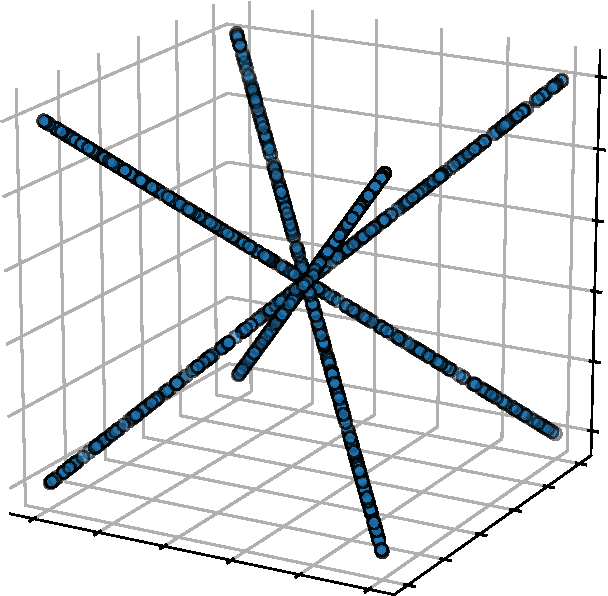
\includegraphics[width=0.14\textwidth]{part2-figures/Cross-3-00-crop-compressed.pdf}}
	\end{subfigure}
	\hfill
    \begin{subfigure}[Dl]
			{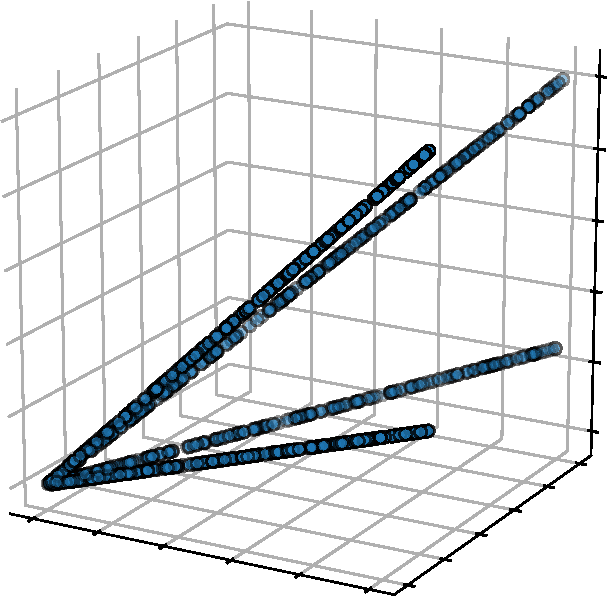
\includegraphics[width=0.14\textwidth]{part2-figures/DoubleLinear_025-3-00-crop-compressed.pdf}}
	\end{subfigure}
	\hfill
	\begin{subfigure}[H]
			{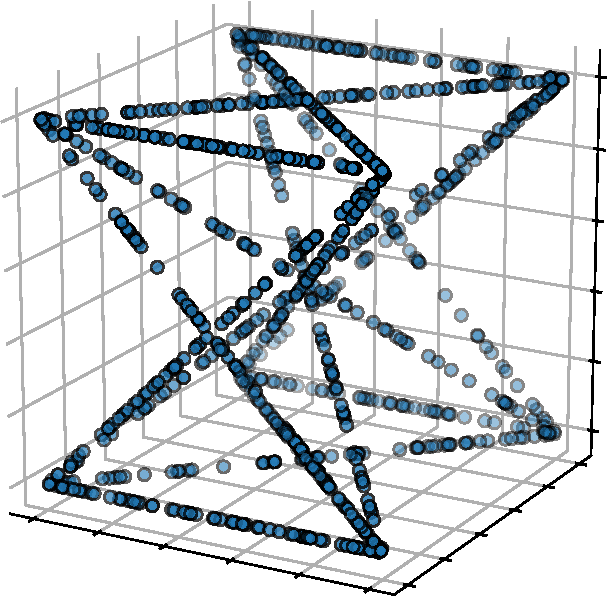
\includegraphics[width=0.14\textwidth]{part2-figures/Hourglass-3-00-crop-compressed.pdf}}
	\end{subfigure}
	\hfill
	\begin{subfigure}[Hc]
			{
			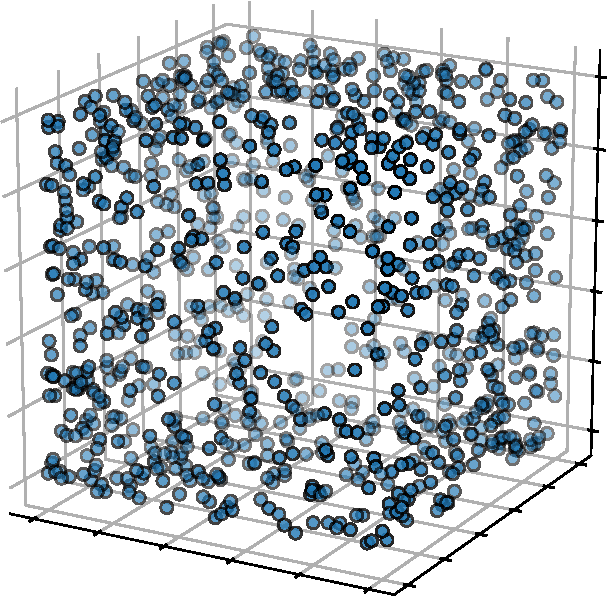
\includegraphics[width=0.14\textwidth]{part2-figures/Hypercube-3-00-crop-compressed.pdf}}
	\end{subfigure}
	\hfill
	\begin{subfigure}[HcG]
			{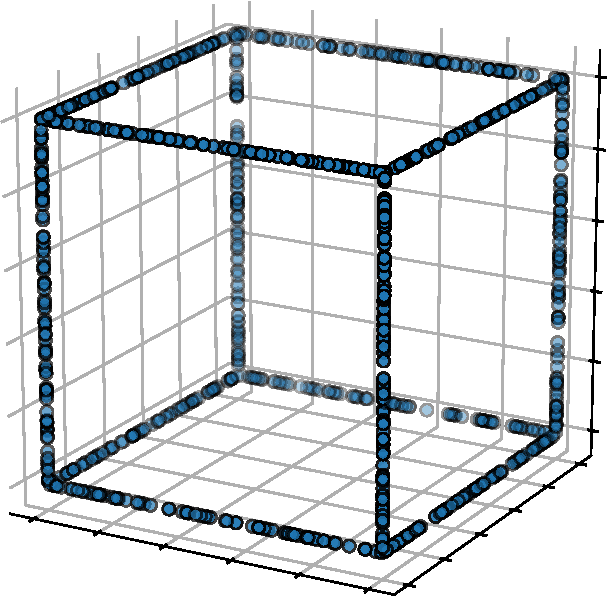
\includegraphics[width=0.14\textwidth]{part2-figures/Hollowcube-3-00-crop-compressed.pdf}}
	\end{subfigure}
	\hfill
	\begin{subfigure}[Hs]
			{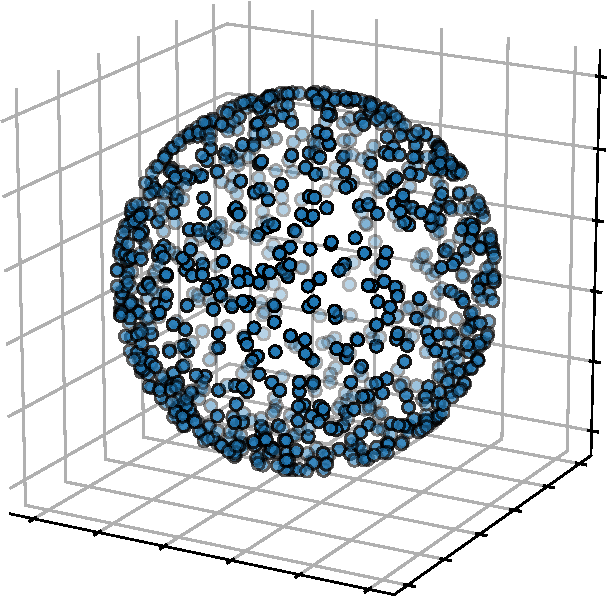
\includegraphics[width=0.14\textwidth]{part2-figures/Sphere-3-00-crop-compressed.pdf}}
	\end{subfigure} 
    
    \begin{subfigure}[L]
			{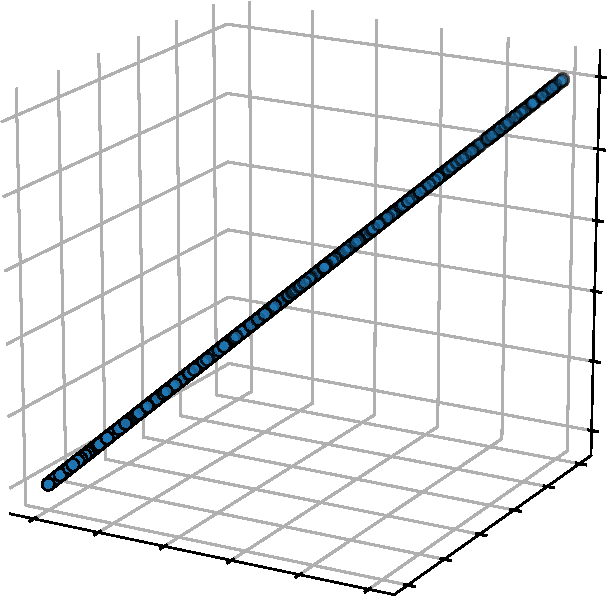
\includegraphics[width=0.14\textwidth]{part2-figures/Linear-3-00-crop-compressed.pdf}}
	\end{subfigure}
	\hfill
    \begin{subfigure}[P]
			{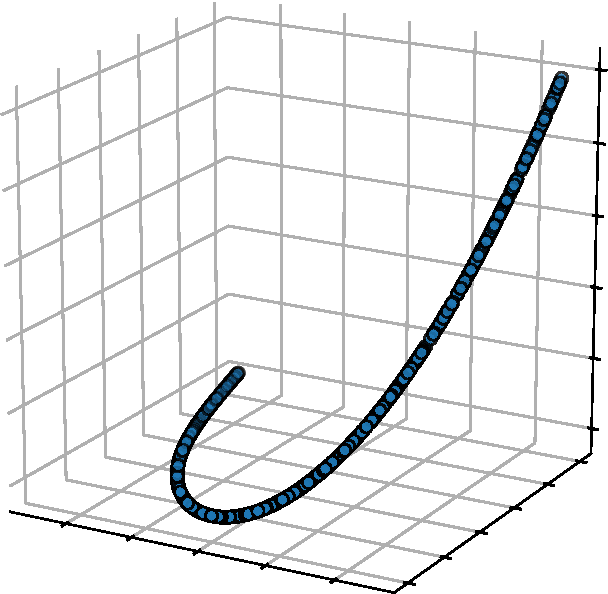
\includegraphics[width=0.14\textwidth]{part2-figures/EvenPower_1-3-00-crop-compressed.pdf}}
	\end{subfigure}
	\hfill
	\begin{subfigure}[S1]
			{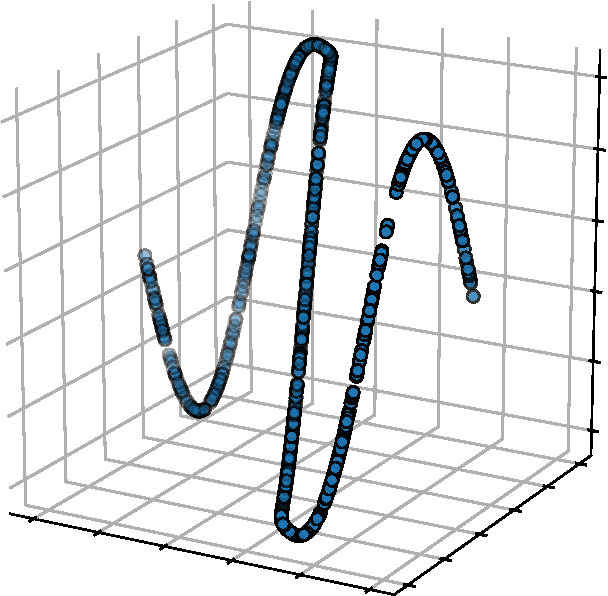
\includegraphics[width=0.14\textwidth]{part2-figures/Sine_1-3-00-crop-compressed.pdf}}
	\end{subfigure}
	\hfill
	\begin{subfigure}[S5]
			{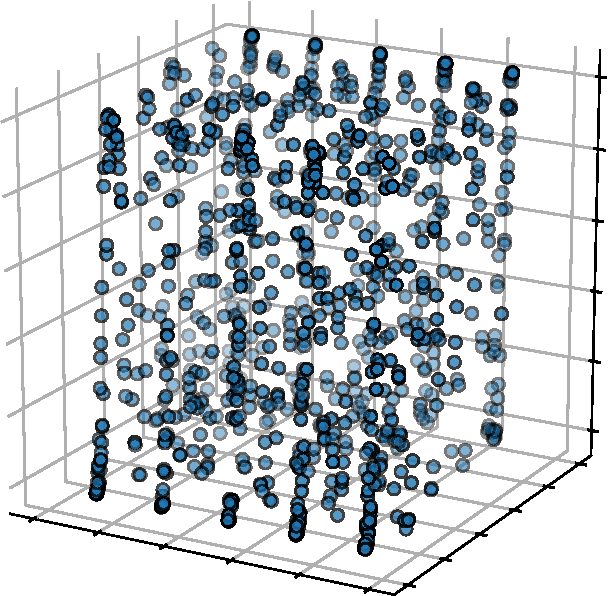
\includegraphics[width=0.14\textwidth]{part2-figures/Sine_5-3-00-crop-compressed.pdf}}
	\end{subfigure}
	\hfill
	\begin{subfigure}[St]
			{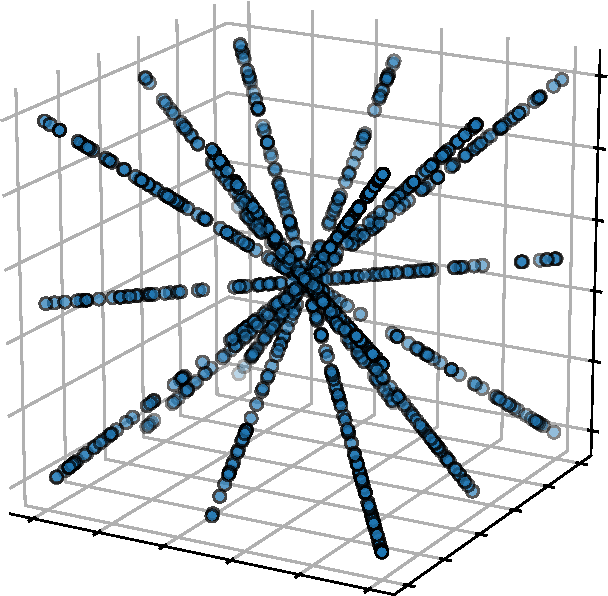
\includegraphics[width=0.14\textwidth]{part2-figures/Star-3-00-crop-compressed.pdf}}
	\end{subfigure}
	\hfill
	\begin{subfigure}[Zi]
			{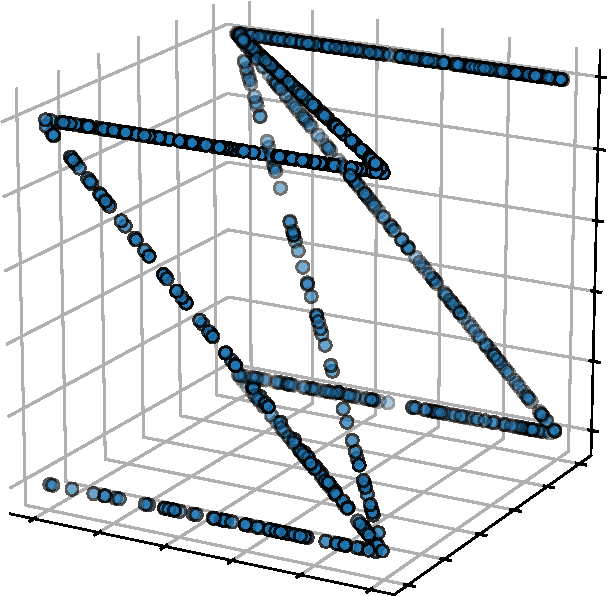
\includegraphics[width=0.14\textwidth]{part2-figures/Zinv-3-00-crop-compressed.pdf}}%\hfill
	\end{subfigure} 
	\caption{An assortment of 12 dependencies (displayed here with three dimensions, $\sigma=0$). C: Cross, Dl: Double linear, H: Hourglass, Hc: Hypercube, HcG: Hypercube Graph, Hs: Hypersphere, L: Linear, P: Parabolic, S1: Sine (P=1), S5: Sine (P=5), St: Star, Zi: Z inversed.}
	\label{fig:deps-plot}
\end{figure}

In our figures, $\text{O}_{\Omega}$ denotes each dependency, where $\text{O}$ stands for the dependency type (e.g., L stands for `Linear'), and $\Omega$ is the discretisation level, i.e., the number of distinct values; $\text{O}$ means that the attributes are numerical. 
`$|\gls{S}|$D' indicates the dimensionality, and $\text{O}^*_\Omega$ indicates that the attributes are categorical, with a number $\Omega$ of nominal values.

\subsection{Evaluation}

In our evaluation, we first compare our three estimators (\gls{MWP}, \gls{KSP} and \gls{CSP}) together. Then, we compare \gls{MWP} to our competitors and present our case study. 

\subsubsection{Specifics of Attributes Types}

We first observe how \gls{MCDE} handles numerical, ordinal, and categorical attributes. 
Figure~\ref{fig:distribution} displays the empirical distribution of \gls{MWP}, \gls{KSP} and \gls{CSP} iterations w.r.t.\ a $2$-dimensional independent (I) and a linearly dependent (L) space. 
Each distribution is estimated as a histogram from $10\,000$ independent iterations. The vertical dashed lines show the means of the distributions, and we display a scatter plot illustrating the corresponding scenario. 

According to Figure \ref{fig:distributuon-independent}, \gls{MWP}, \gls{KSP} and \gls{CSP} values are uniformly distributed in the case of an independent subspace, with a few exceptions: 
First, the \gls{CSP} values are all close to $0$ in the case of numerical attributes. 
Since each point is unique, they are all treated as a single category, 
and the Chi-Squared test does not have power in this setting. 
We observe the same effect with L (in \ref{fig:distributuon-linear}). 
Second, we see that the values of \gls{MWP} and \gls{CSP} are also $0$ with I$_1$. 
This corresponds to the desired behaviour. In this situation, every observation in the subspace is equal, so contrast is undefined. 
\gls{KSP} assumes that values are continuous, and thus does not handle this case.

Also, we can see from \ref{fig:distributuon-linear} that the \gls{KSP} values are generally closer to $1$ with L and L$_{10}$. 
This indicates a larger power than \gls{MWP} and \gls{CSP}. 
However, we can see that the \gls{CSP} distribution does not change between L$_{10}$ and L$^*_{10}$, while the mean of the \gls{MWP} and \gls{KSP} distribution decreases significantly. 
Thus, \gls{CSP} detects dependency from categorical attributes better than \gls{MWP}/\gls{KSP}. 

\begin{figure}
	\begin{subfigure}[Independent]
			{\label{fig:distributuon-independent}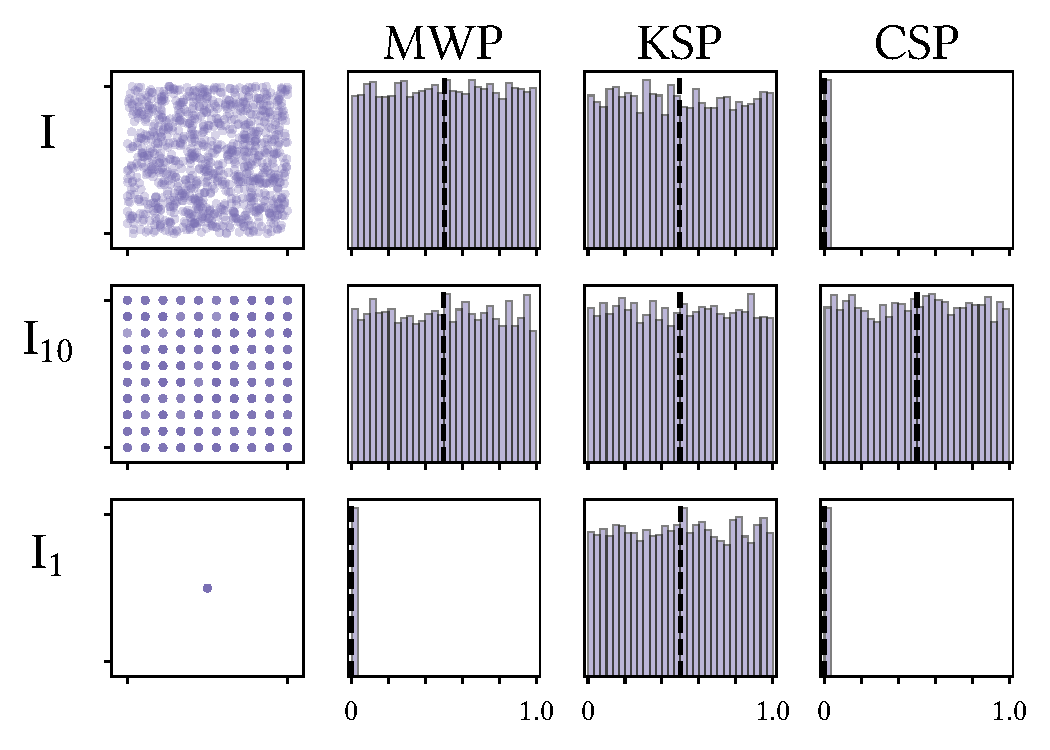
\includegraphics[width=0.49\textwidth, trim=0 0 0 0.5cm]{part2-figures/contrast_distribution_data_I_thesis-compressed.pdf}}
	\end{subfigure}
	\hfill
	\begin{subfigure}[Dependent (Linear, $\sigma=0.4$)]
			{\label{fig:distributuon-linear}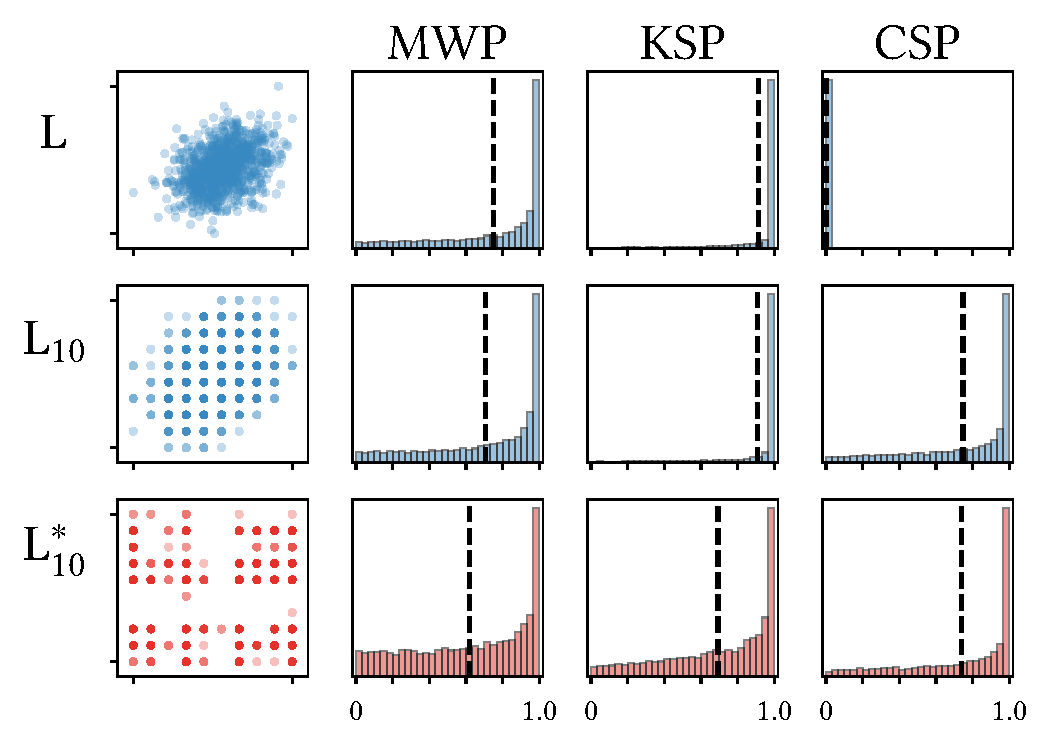
\includegraphics[width=0.49\textwidth, trim=0 0 0 0.5cm]{part2-figures/contrast_distribution_data_L_thesis-compressed.pdf}}
	\end{subfigure} 
	\caption{Distribution of the contrast estimation iterations ($|\gls{S}| = 2$).} 
	\label{fig:distribution}
\end{figure}

\subsubsection{Statistical Power of \gls{MWP}, \gls{KSP} and \gls{CSP}}

We first look at the statistical power of \gls{MWP}, \gls{KSP} and \gls{CSP} with confidence level $\gamma = 0.95$  against a linear dependency of increasing dimensionality $|\gls{S}|$, discretisation level $\Omega$, and noise level $\sigma$. 
Please note that the figures are best seen in colour. 
The expectation is that the scores and statistical power are high for noiseless dependencies, i.e., the left side of the plot is blue, and decrease gradually as we add noise. A noise level $\sigma = 1$ is comparably high since the data is scaled to $[0,1]$. Thus, the right side of the plot should be red, standing for low scores, or low power. 
From Figure \ref{fig:power} (upper part), we see that \gls{MWP} without marginal restriction does not work well in high-dimensional and highly discretised spaces. 

The marginal restriction alleviates this problem to some extent, in particular for numerical subspaces. 
In fact, as dimensionality increases, it becomes more and more likely that the points selected in the slice are `at the centre' of the distribution. 
As a result, the mean of the point in the slice and the point outside of the slice become nearly equal, leading to low power with the Mann-Whitney U test, and thus a slight performance decrease of \gls{MWP}. %In general, MWP has less power than KSP. 
This calls for further research on the \gls{MWP} slicing scheme, or alternatives to the Mann-Whitney U test. 
Nonetheless, the results indicate that \gls{MWP} with marginal restriction works well against numerical attributes. Next, we see that \gls{KSP} has high power in every case, although slightly decreasing with $\Omega$. 
\gls{CSP} does not work with numerical spaces but has more power in discrete spaces. \gls{CSP} works best with categorical attributes. 
% We also see that KSP is more robust against noise. 

We now compare the power of our estimators against the assortment of dependencies from Figure \ref{fig:deps-plot}. 
\gls{CSP} does not apply to numerical attributes. Thus, for comparability, we discretise the values with $\Omega = 10$. We can see from Figure \ref{fig:power} (lower part) that \gls{KSP} consistently has more power than \gls{MWP}, and even alleviate some of its drawbacks, such as the low power against the noiseless Hypercube (Hc). 
\gls{CSP} generally has less power than \gls{KSP} but can detect categorical dependencies. 

Our experiments show that \gls{MWP} has a slight performance decrease in high-dimensional discrete spaces. 
\gls{KSP} seems to perform better, but its statistical power decreases with discretisation. 
Overall, we recommend to use \gls{KSP} for numerical and ordinal data but to use \gls{CSP} for categorical data. 
\gls{MWP} still is a valid alternative with numerical attributes. %In the future, it would be interesting to come up with better subspace slicing schemes for MWP. 

\begin{figure}
	\centering 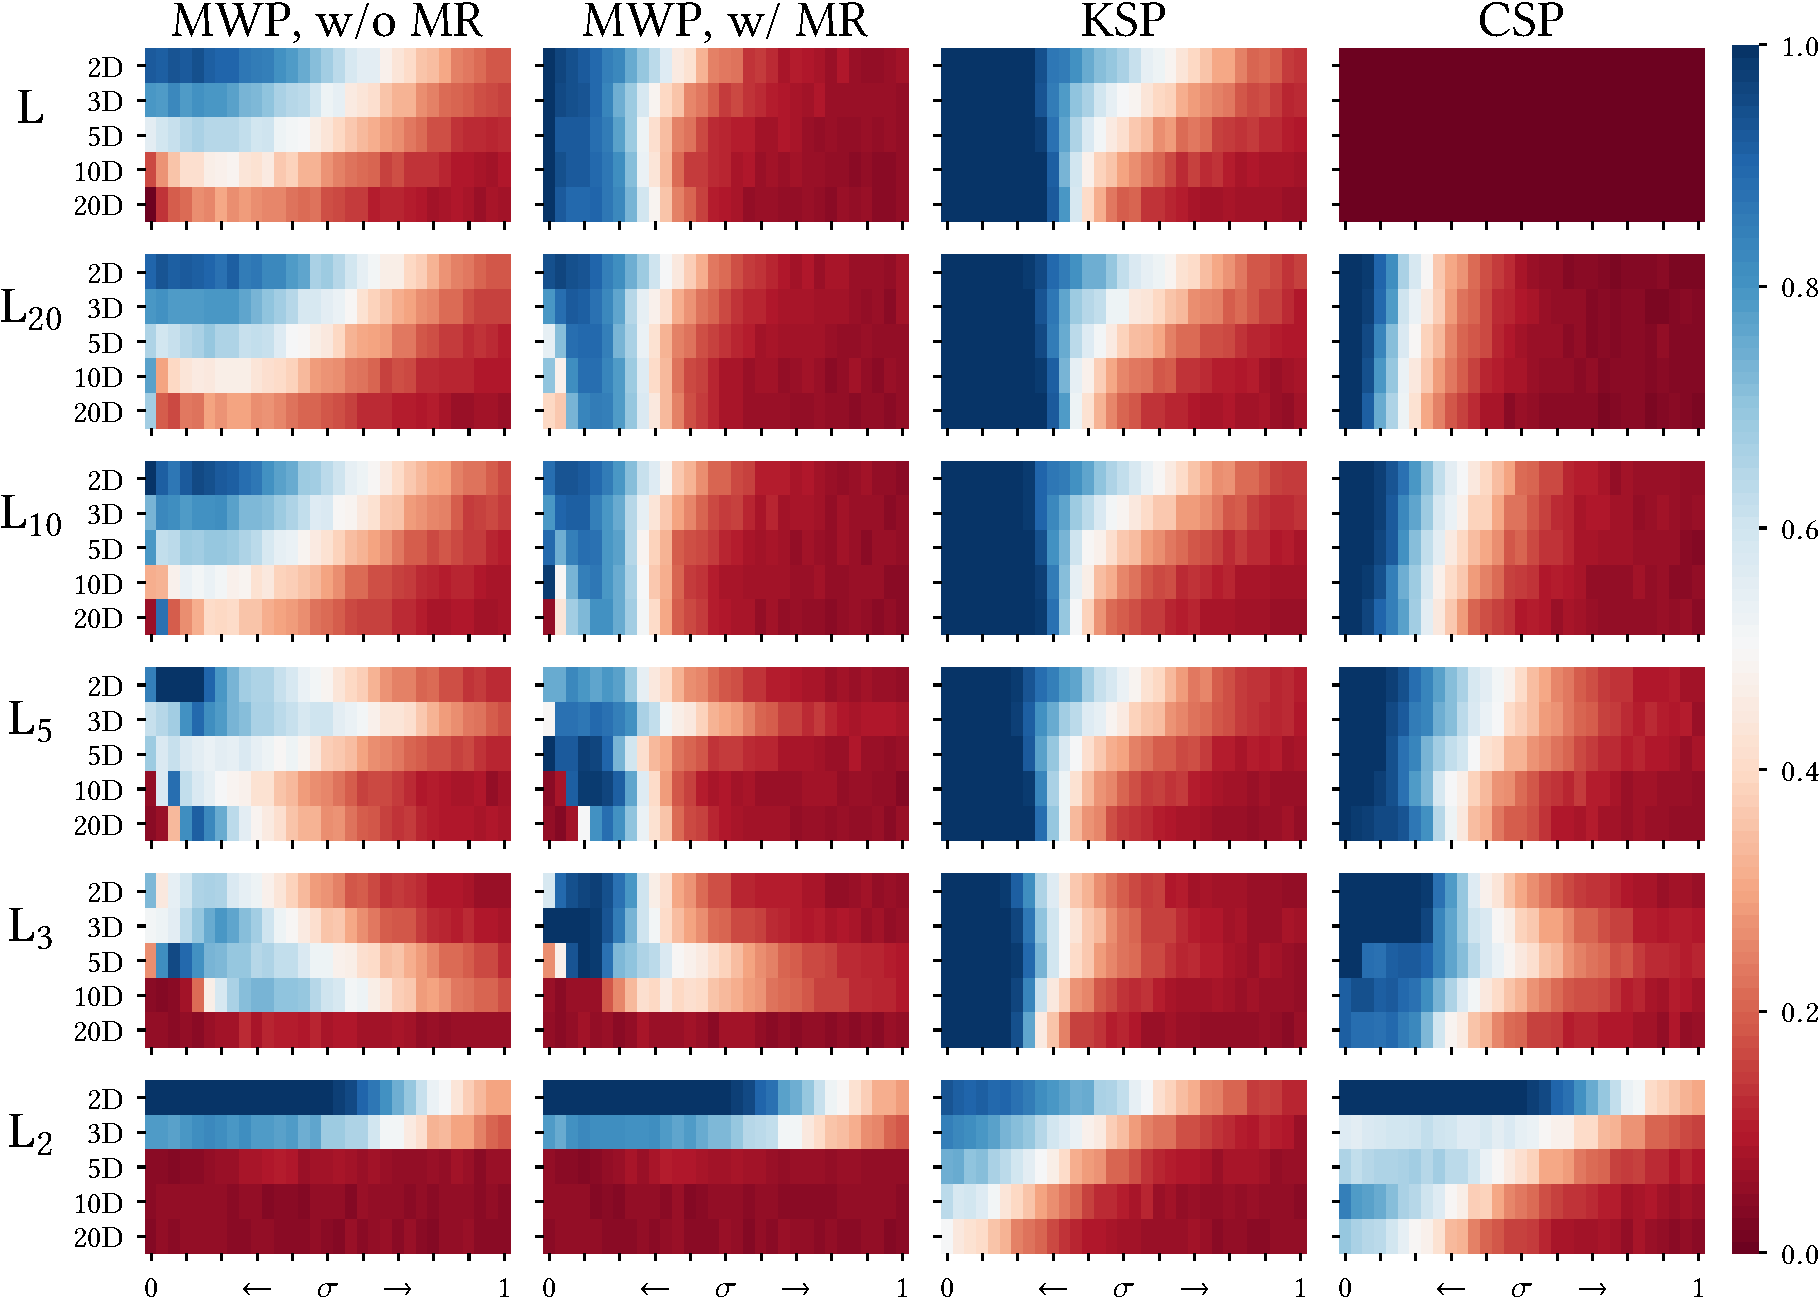
\includegraphics[width=0.98\linewidth, trim=0 0.25cm 0 0.25cm]{part2-figures/power_L_thesis-crop-compressed.pdf} \hfill \\
	\vfill
	\hfill
	\vfill
    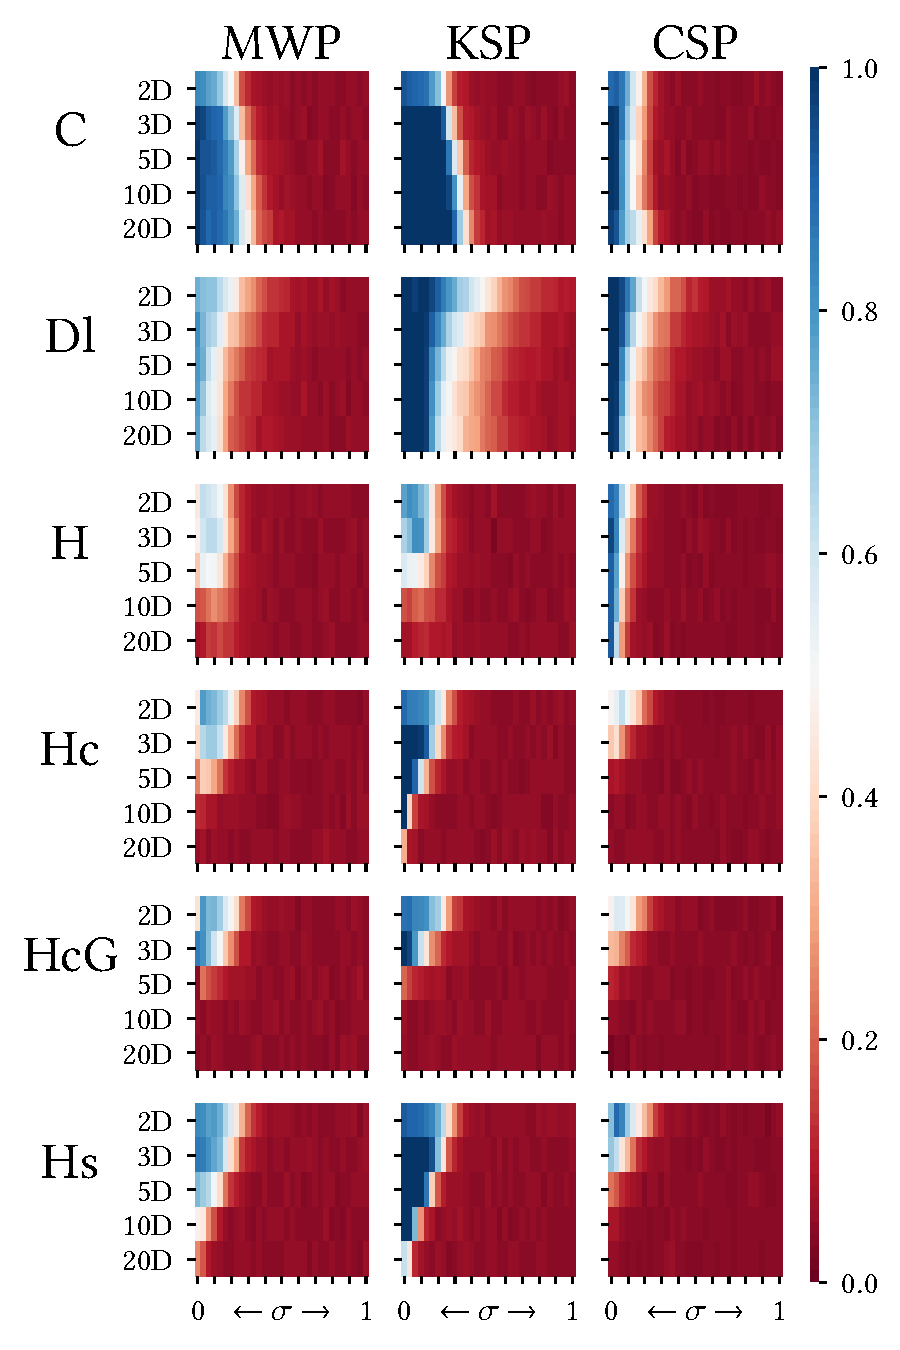
\includegraphics[width=0.49\linewidth, trim=0 0.25cm 0 0.25cm]{part2-figures/power_1_thesis-compressed.pdf}
    \hfill
    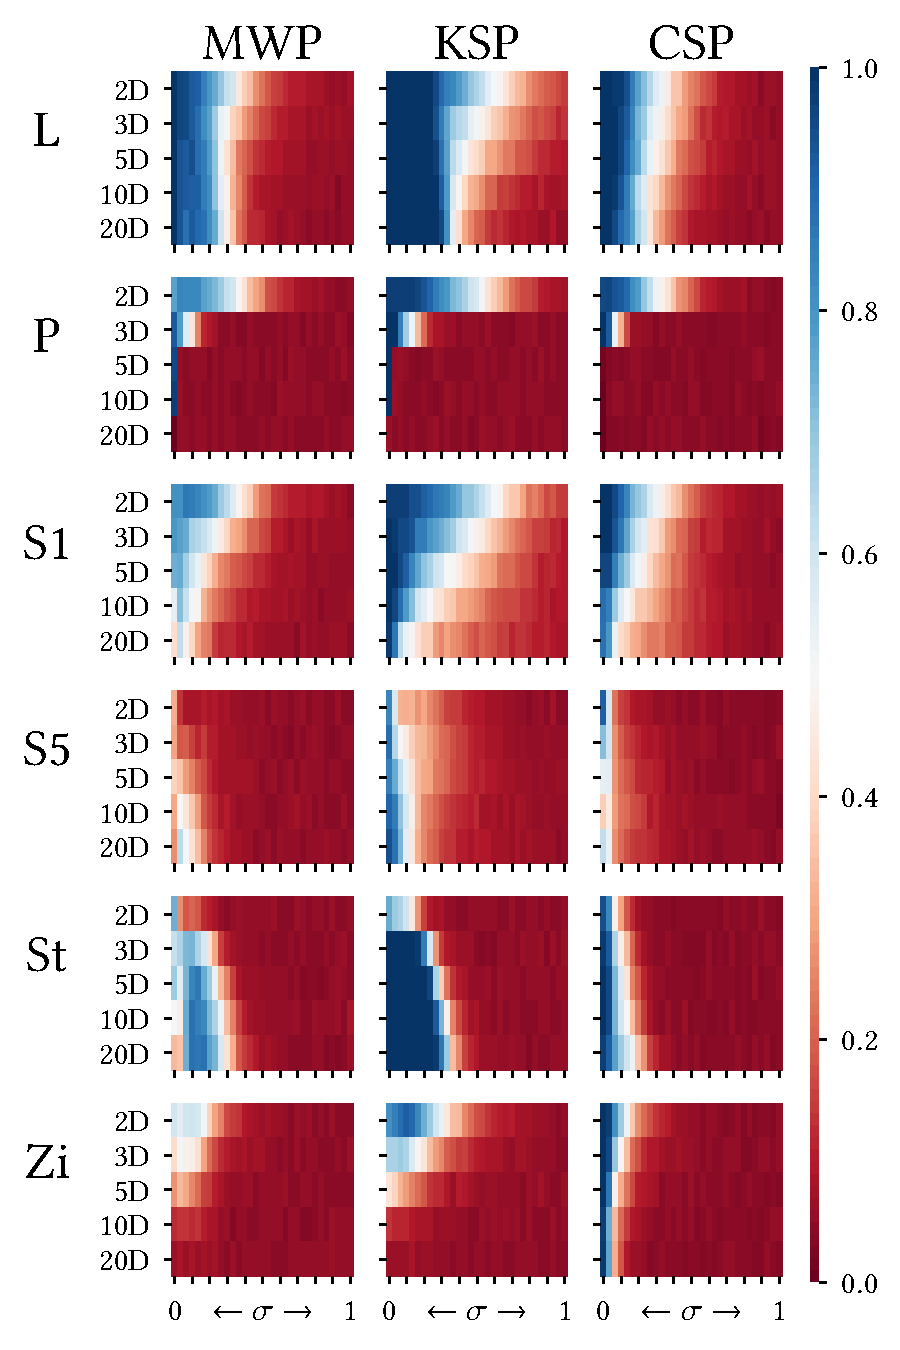
\includegraphics[width=0.49\linewidth, trim=0 0.25cm 0 0.25cm]{part2-figures/power_2_thesis-compressed.pdf}
    \hfill
    \caption{Power of \gls{MWP}/\gls{KSP}/\gls{CSP} against continuous/discrete linear distributions (upper part) and our assortment of dependencies (lower part).}
    \label{fig:power}
\end{figure} 

\subsubsection{Influence of parameters, $\gls{w}$, $M$ and $|\gls{S}|$}

\begin{figure}
	\centering
	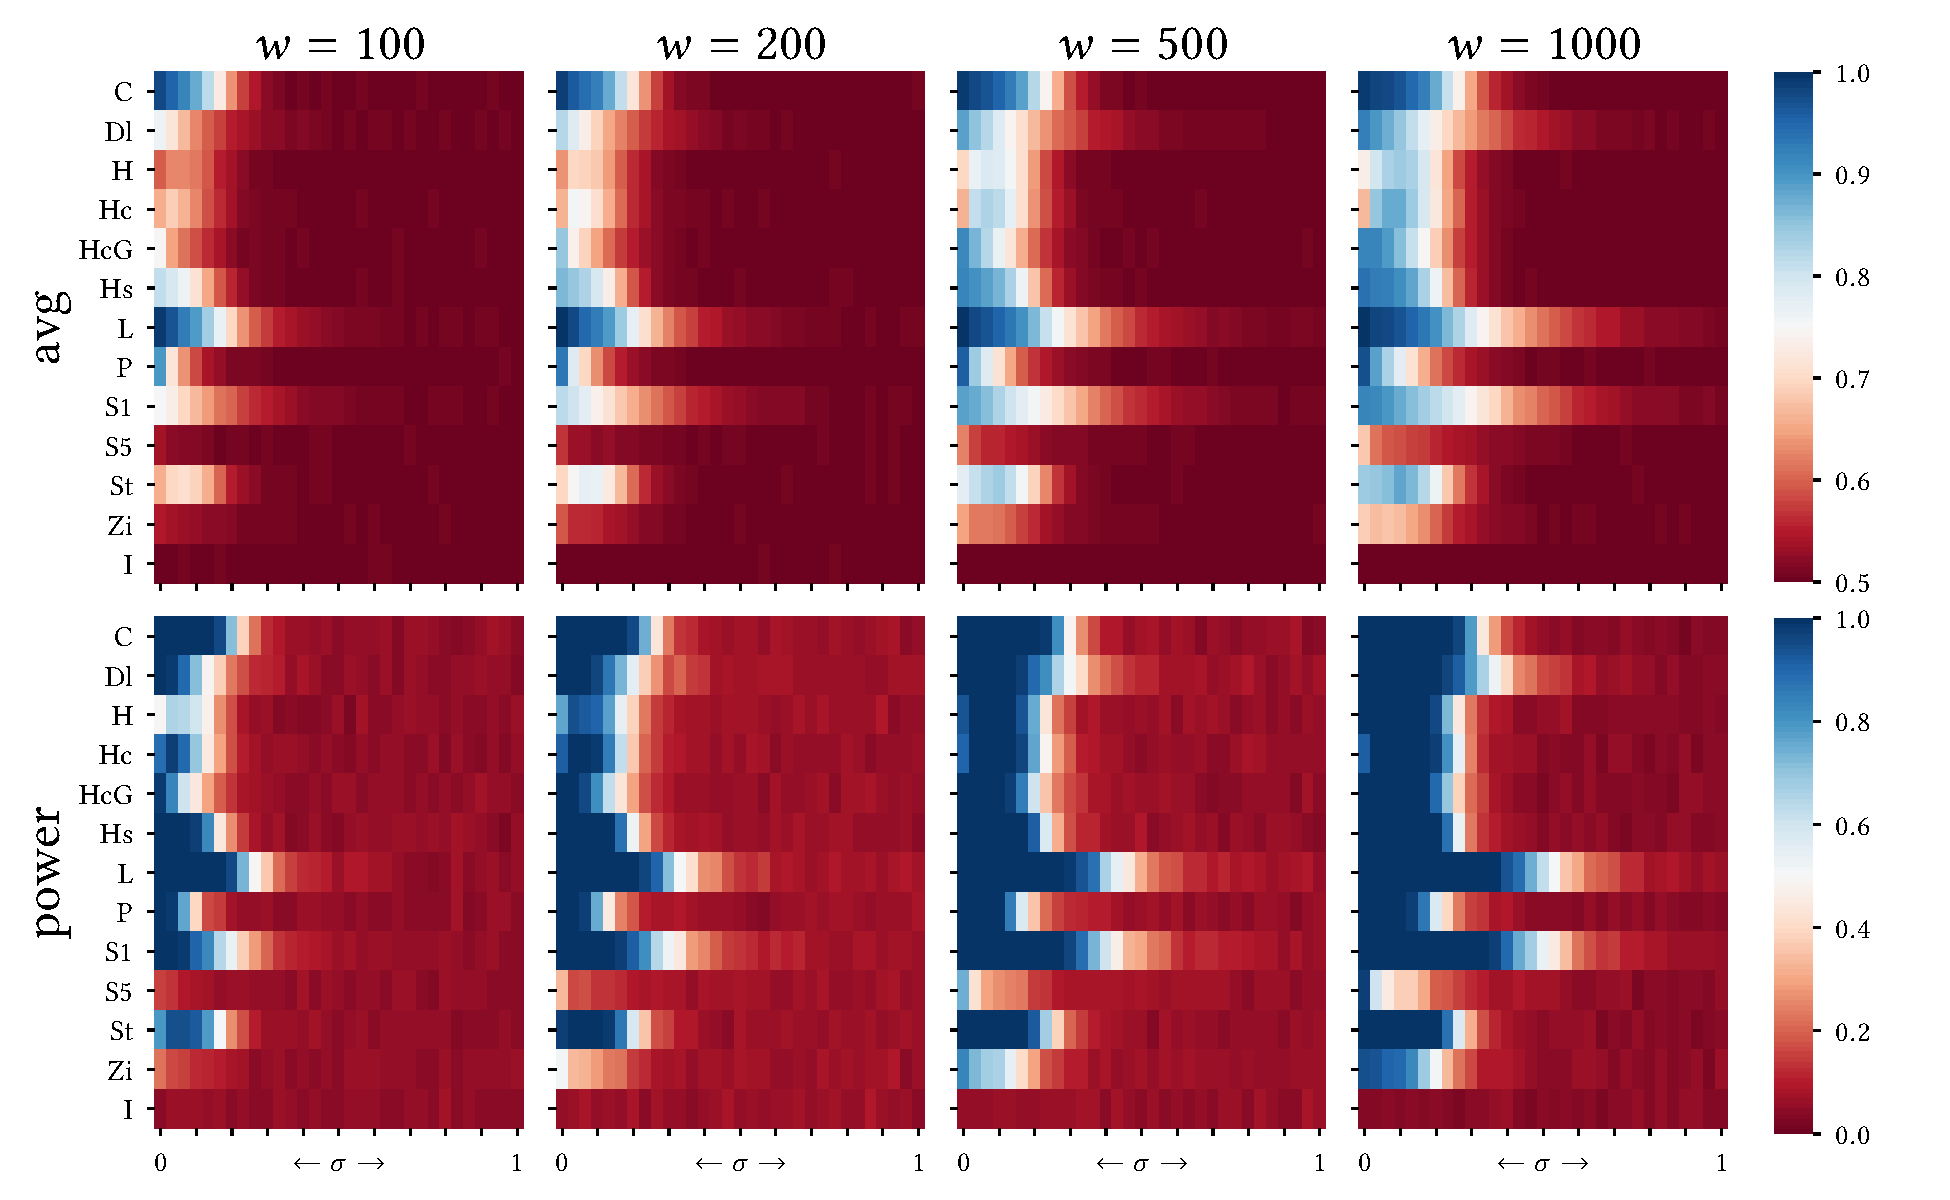
\includegraphics[width=\linewidth, trim=0 0.5cm 0 0.5cm]{part2-figures/Fig5_1-2_thesis-compressed.pdf}
	\caption{Power of \gls{MWP} w.r.t. $\gls{w}$.}
	\label{fig:N_MWP}
\end{figure}

\begin{figure}[ht]
	\centering
	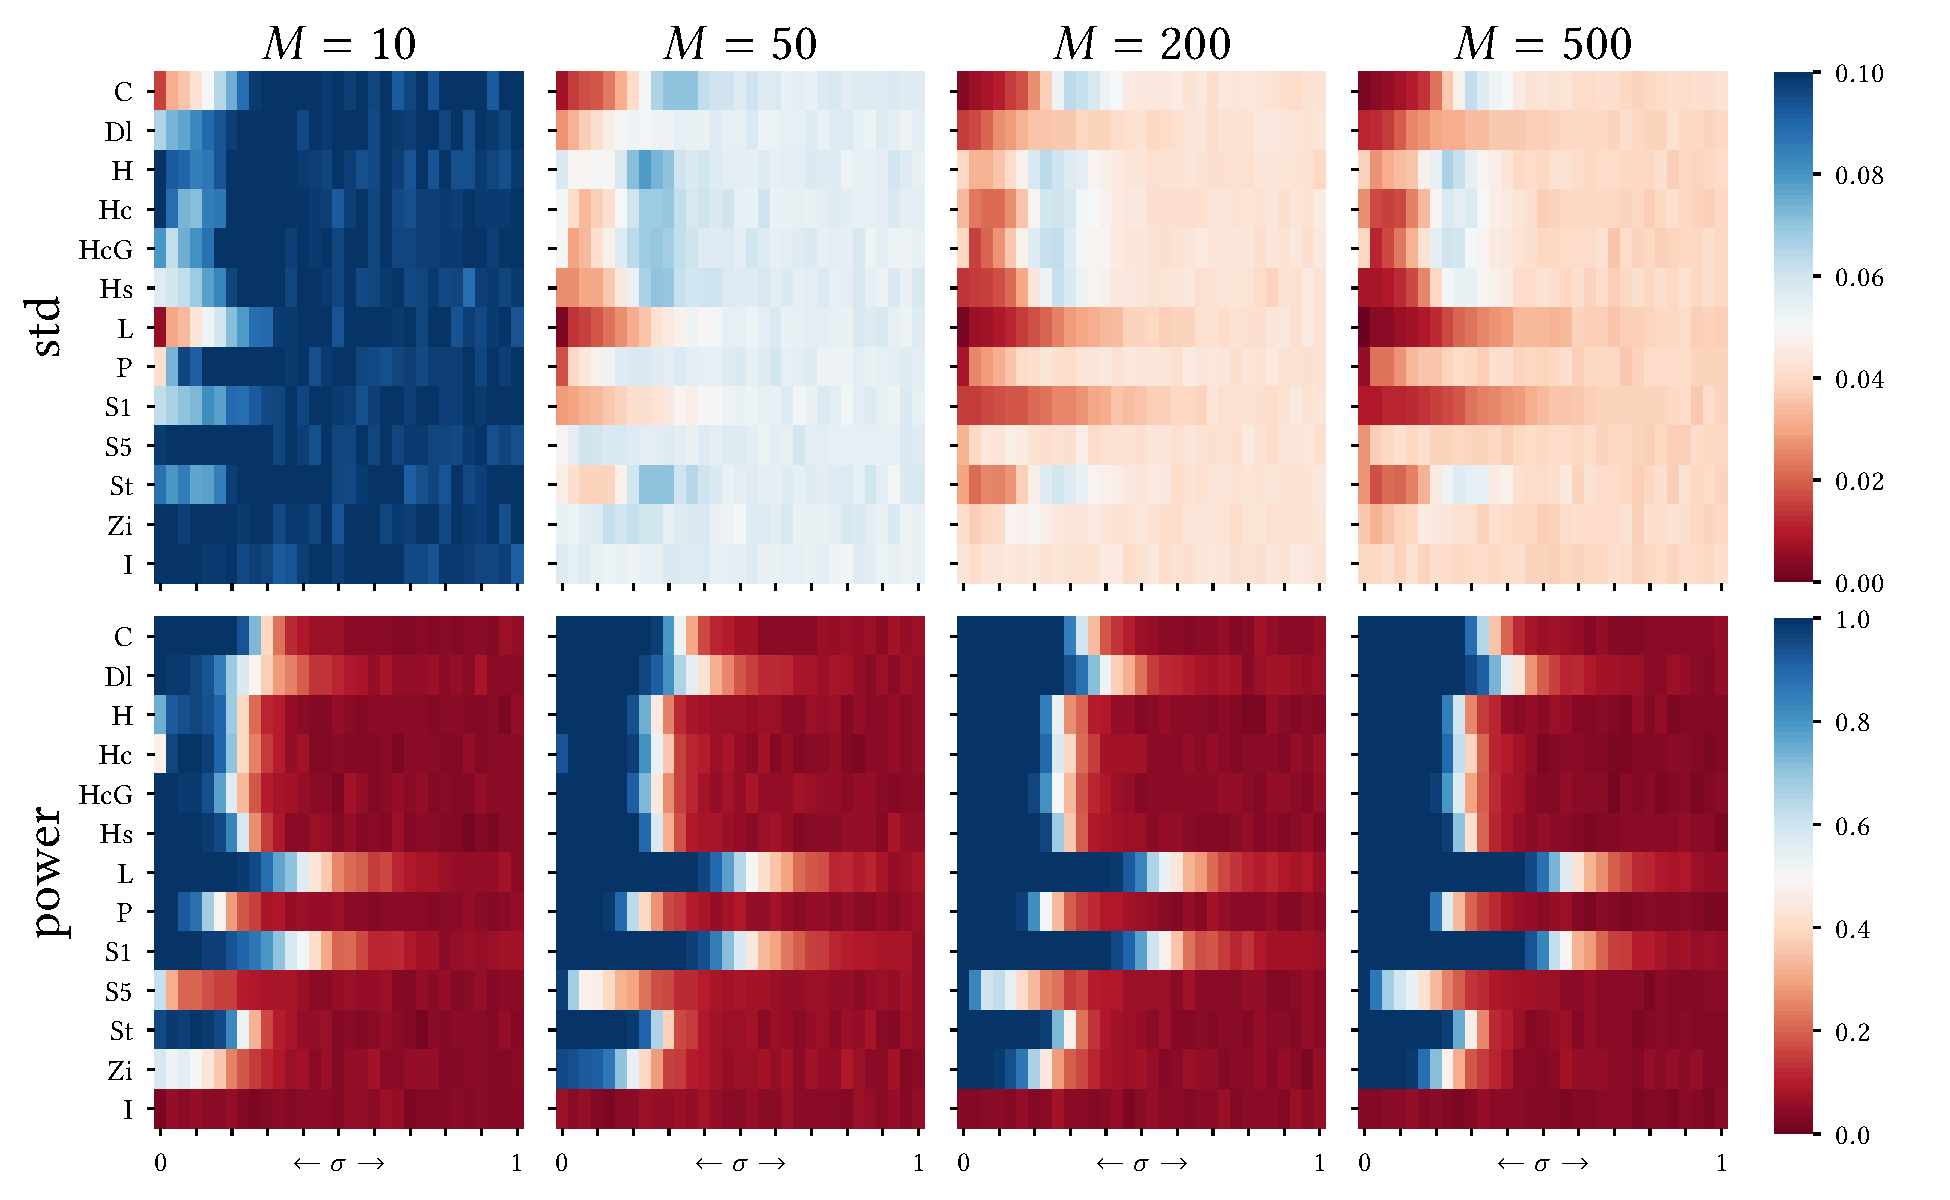
\includegraphics[width=\linewidth, trim=0 0.5cm 0 0.5cm]{part2-figures/Fig5_2-2_thesis-compressed.pdf}
	\caption{Power of \gls{MWP} w.r.t. $M$.}
	\label{fig:M_MWP}
\end{figure}

Figure~\ref{fig:N_MWP} shows that power globally increases with $\gls{w}$, but it is still high for most dependencies with low $\gls{w}$, provided noise is moderate. 
As we can see, the average score of \gls{MWP} tends to increase with $\gls{w}$, which explains the gain in power. That is because \gls{MWP} is sensitive (\hyperlink{R6}{\textbf{R6}}), as we discuss in \mbox{Section \ref{sensitivity}}.
Similarly, Figure~\ref{fig:N_MWP} shows that power increases slightly as $M$ increases, but the effect is visible only for S5 and Zi. We can explain this increase of power easily by the fact that the standard deviation of \textit{\gls{MWP}} decreases, which is what Theorem \ref{"th:hoeffding-chernoff-contrast"} predicted: with more iterations, the values concentrate around $\mathcal{C}$. 
In the end, we see that \gls{MWP} is already useful for small $\gls{w}$ or small $M$, even though more iterations or more data samples yield higher power when data is noisy. 

\begin{figure}
	\centering
	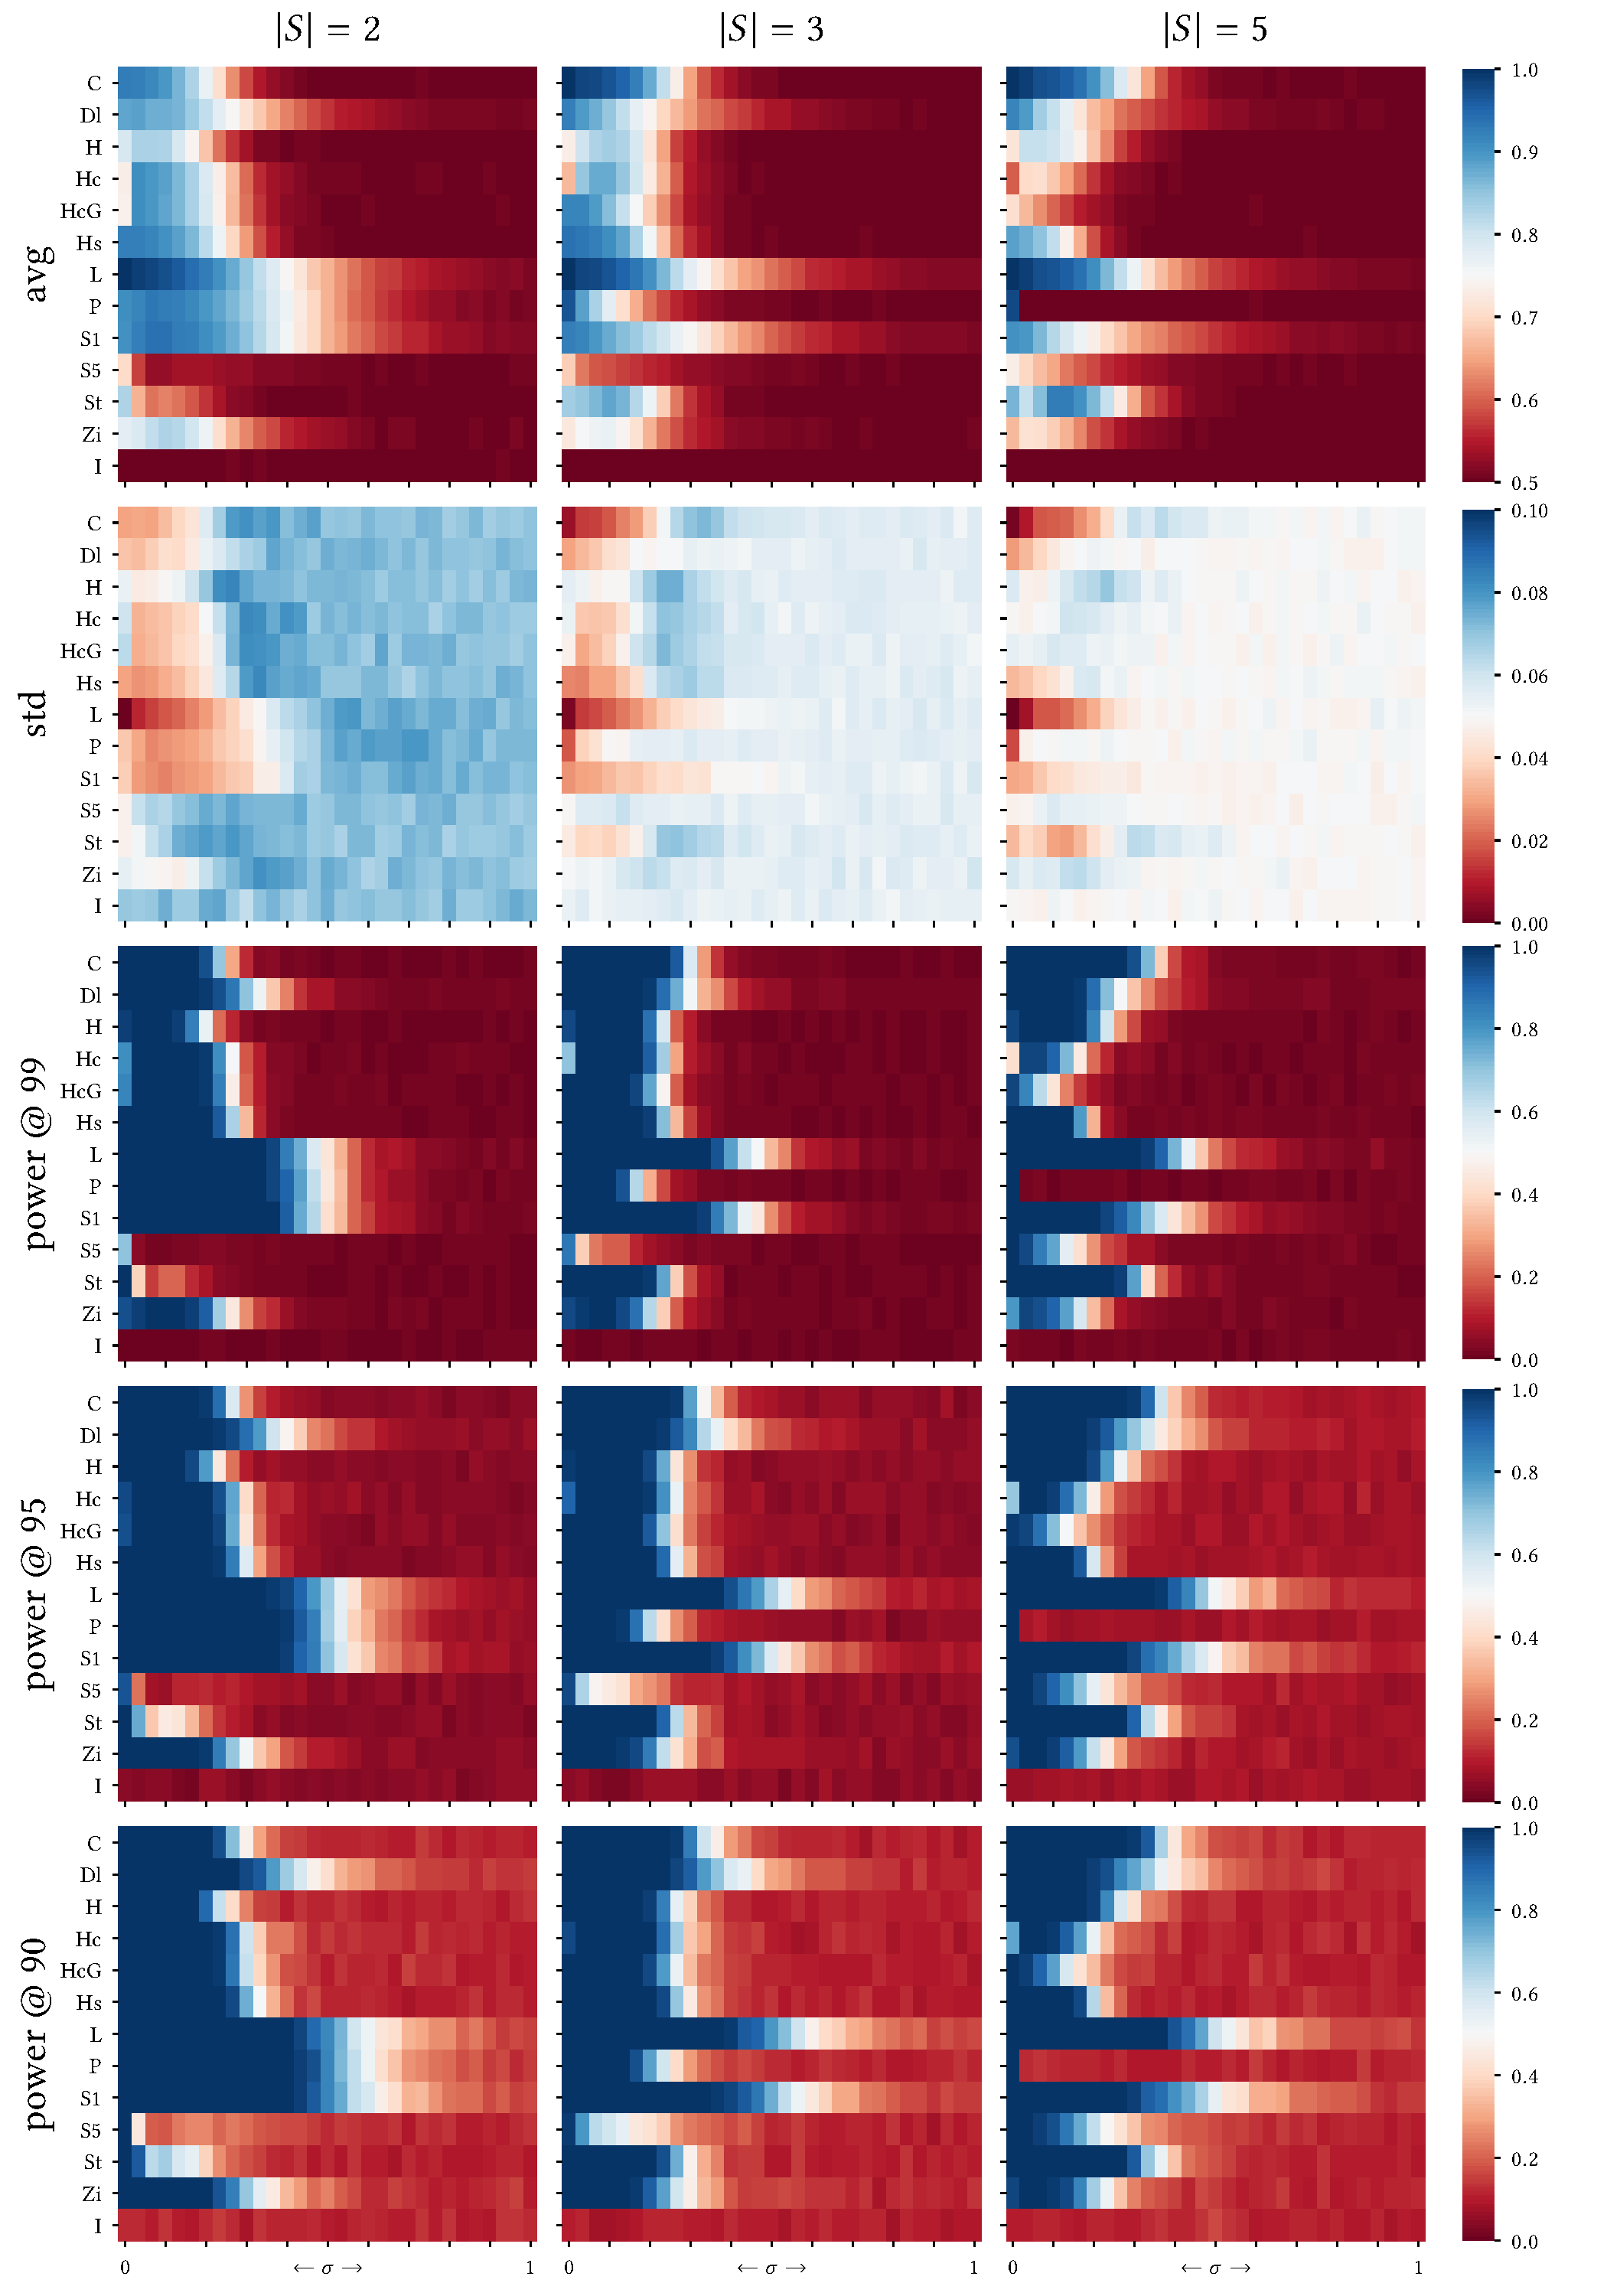
\includegraphics[width=1.0\linewidth]{part2-figures/Fig4-3_thesis-compressed.pdf}
	\caption{\gls{MWP} w.r.t. dimensionality $|\gls{S}|$.}
	\label{fig:momentsMWP}
\end{figure}

Figure~\ref{fig:momentsMWP} graphs the evolution of \gls{MWP} for $|\gls{S}| = 2,3,5$. 
As we see, the average \gls{MWP} decreases gradually for each dependency. The same level of noise does not seem to affect each estimate equally, also regarding dimensionality. 
For instance, the estimates of L, P and S1 are larger at $|\gls{S}|=2$.
While the estimates of Hc, HcG, P and Zi decrease with increasing $|\gls{S}|$, they increase for C and St. While some dependencies (e.g., Hc, HcG) appear to have lower contrast without noise, we see that this effect is not as visible when we decrease the threshold for measuring power. 
The standard deviation of \gls{MWP} increases with noise and decreases with $|\gls{S}|$. In particular, L, C and Hs have a low standard deviation. This means that fewer iterations are required to estimate stronger dependencies. 
Power does not seem to vary much with dimensionality for most dependencies. It decreases with $|\gls{S}|$ for Hc, HcG, Hs, P and Zi, while it increases for C, S5 and St. 

All in all, each dependency yields a score larger than I up to a certain level of noise, leading to high power. Thus, \gls{MWP}, and, by extension, \gls{MCDE}, are general-purpose (\hyperlink{R2}{\textbf{R2}}).

\subsubsection{Comparison to Competing Approaches}

\begin{figure*}
	\centering
	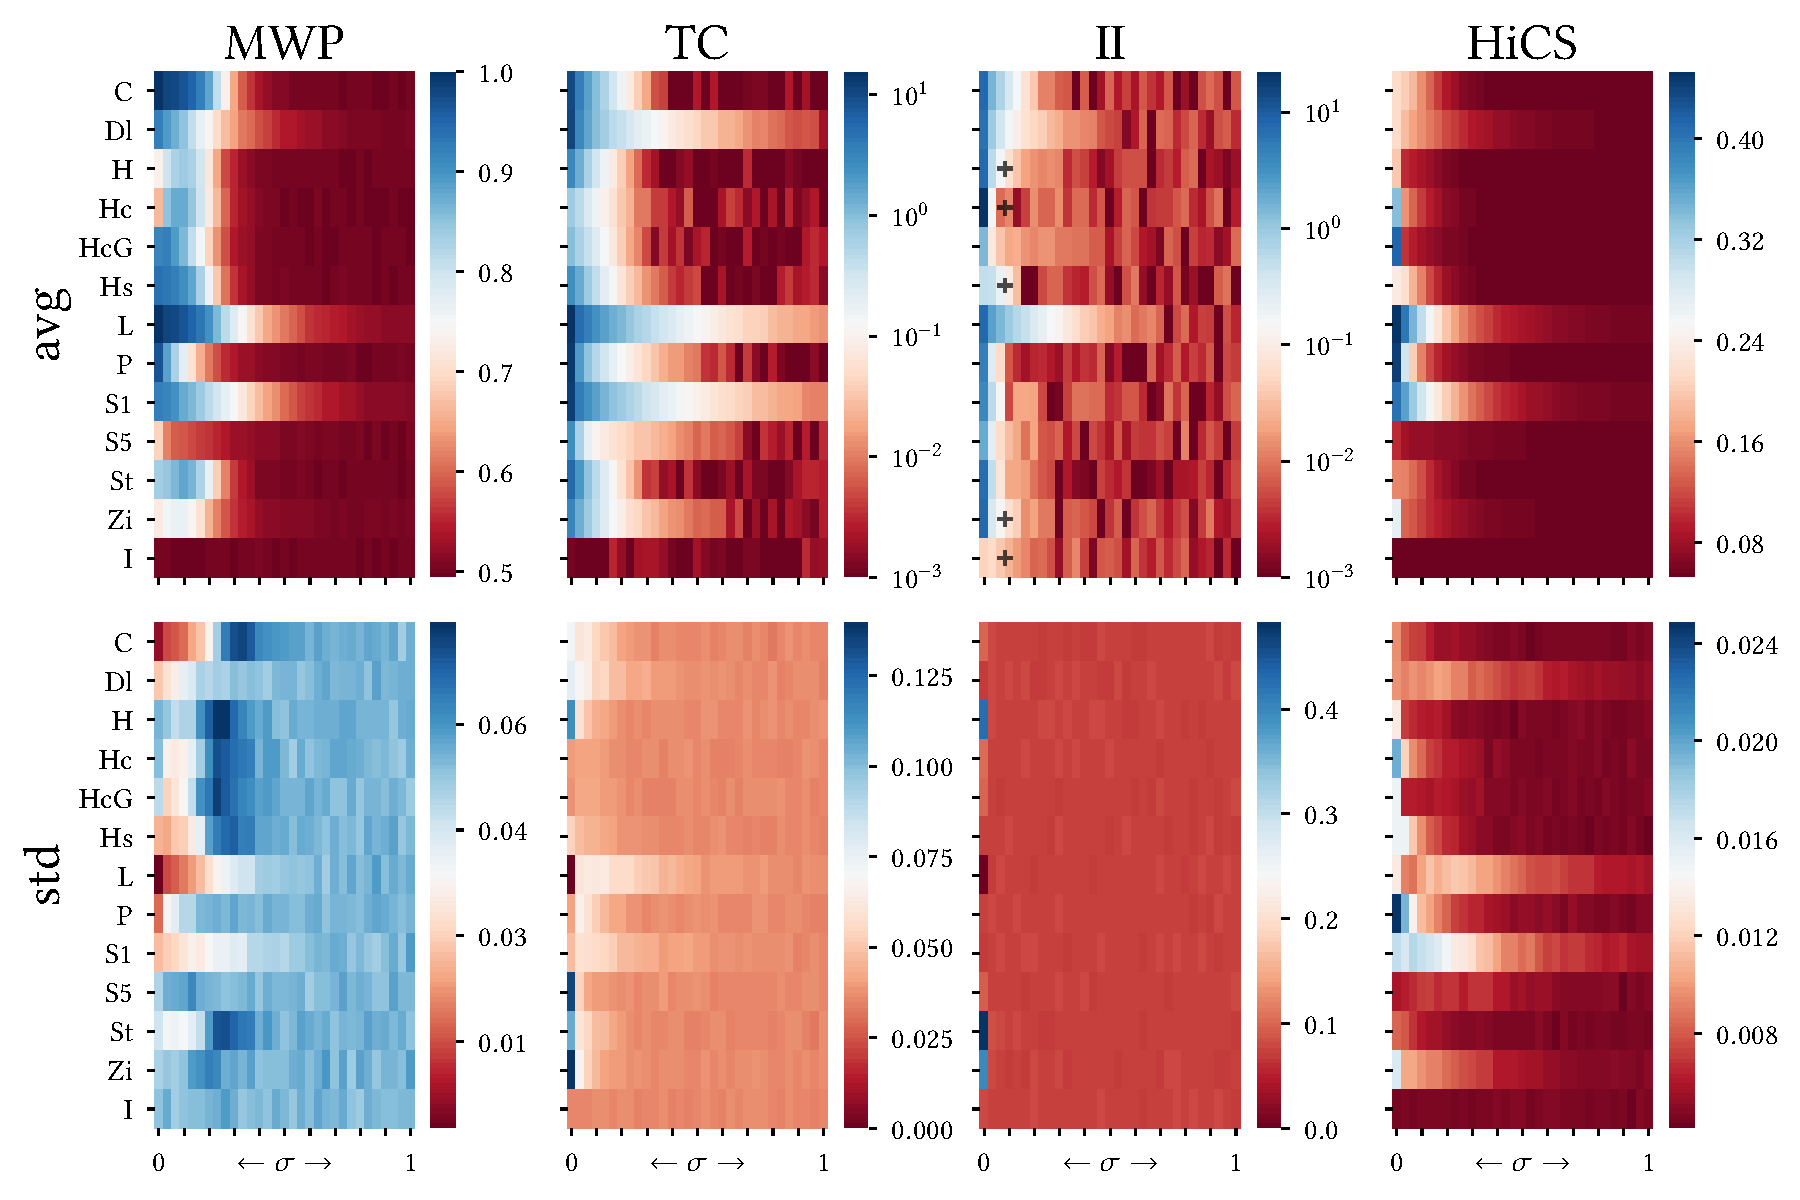
\includegraphics[width=1.0\linewidth]{part2-figures/Fig6_large_1-2_thesis-compressed.pdf}
	\hfill
	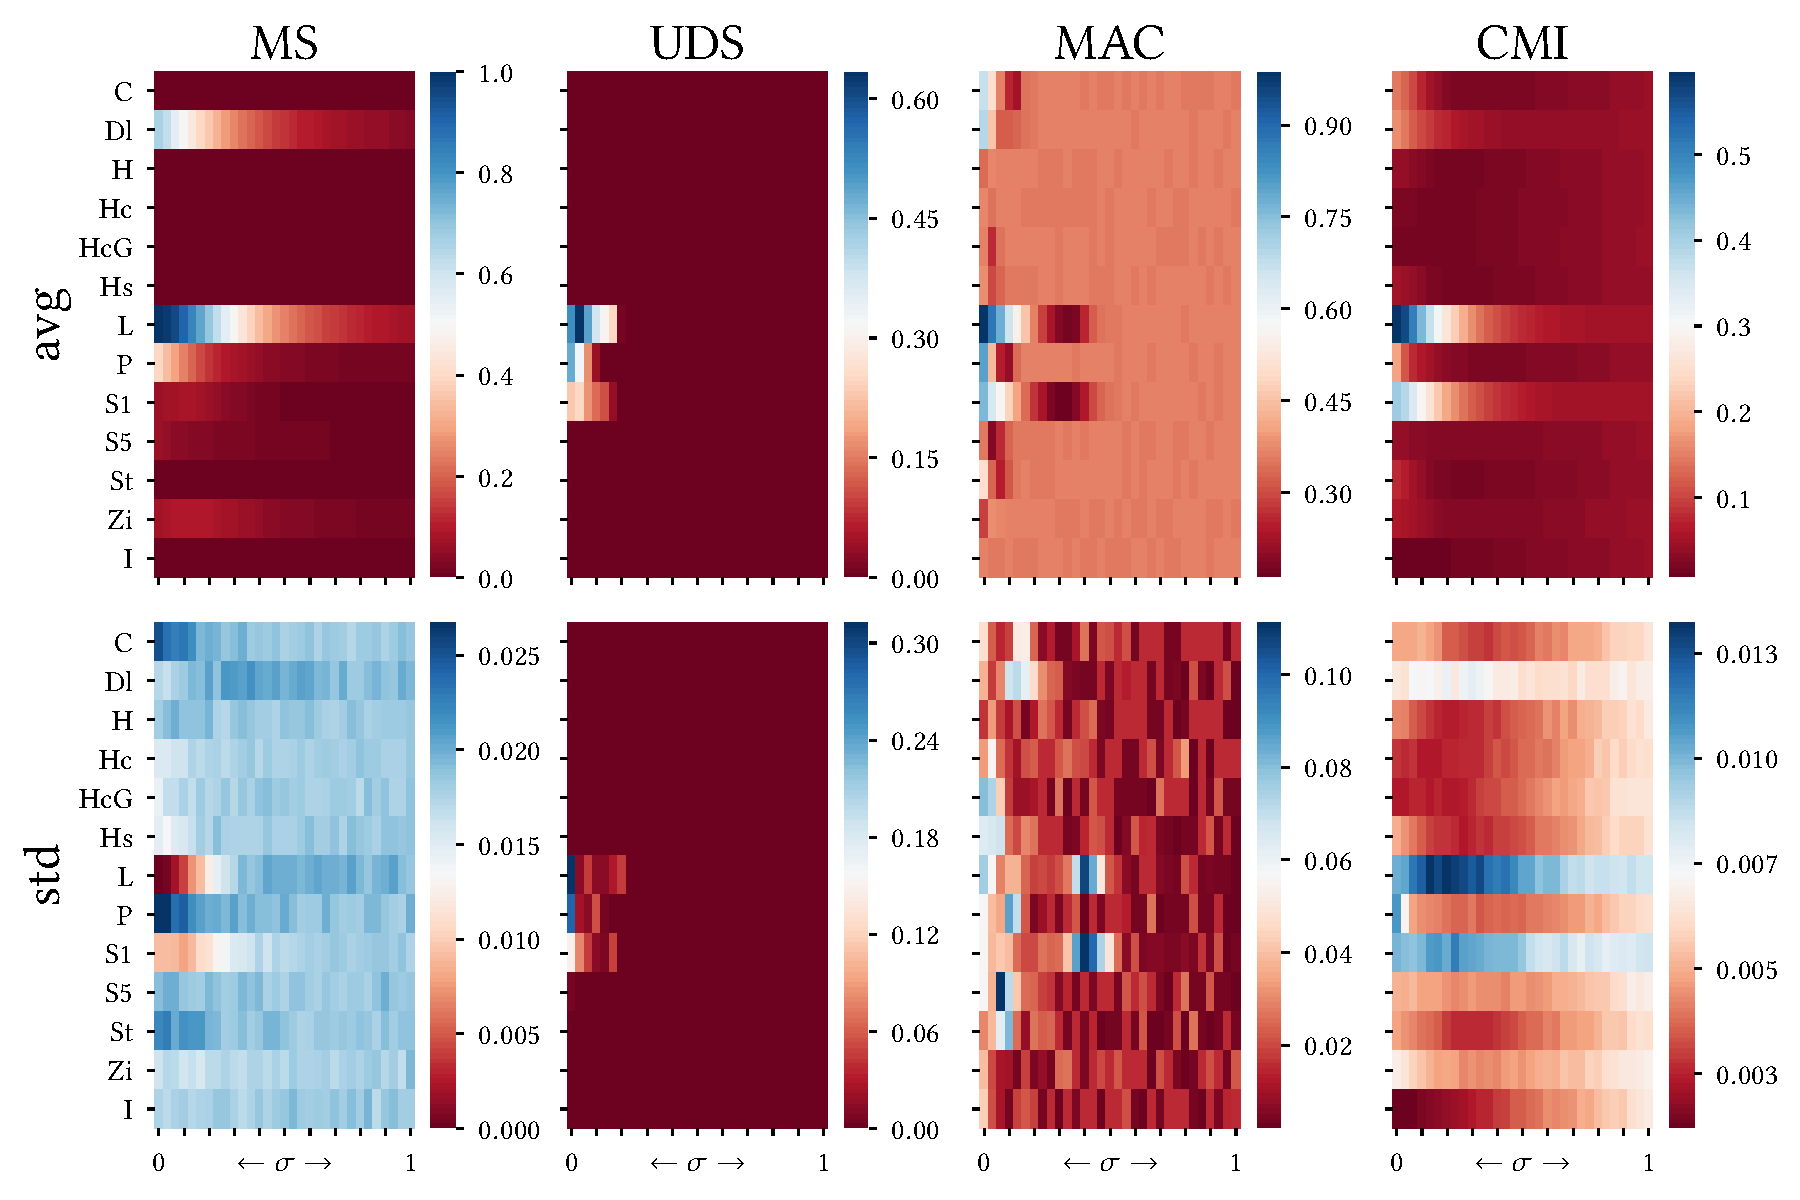
\includegraphics[width=1.0\linewidth]{part2-figures/Fig6_large_2-2_thesis-compressed.pdf}
	\caption{Distribution of dependency estimation scores, $|\gls{S}|=3$.}
	\label{fig:contrast_all}
\end{figure*} 

We compare the score distribution for each competing approach with \gls{MWP} in Figure~\ref{fig:contrast_all}. First, we see that the average score of \gls{MWP} is most similar to \gls{TC}. However, \gls{TC} is unbounded, and its scores follow a logarithmic scale. This means that the estimates of \gls{TC} change very abruptly. We see that \gls{MWP} scores are slightly smaller for noiseless dependencies with many ties w.r.t. marginal distributions, such as H and Hc, which we attribute to the correction for ties in the Mann-Whitney U test.
 
\gls{II} can yield positive or negative values. %Since both cases are interesting, 
We visualise the absolute value of \gls{II} with a logarithmic scale. We mark the dependencies which obtain a positive score in their noiseless form with a plus sign.
\gls{II} assigns high scores to every noiseless dependency. However, the score decreases rapidly with noise, except for L.

\gls{HiCS} shows a similar behaviour as \gls{MWP}, except that the scores decrease faster, and that many dependencies start with a relatively 
low score, even in the noiseless form, such as C, Dl, H,  Hs, S5 and St. 
Next, \gls{MS} and \gls{UDS} are restricted to monotonous and bijective functional relationships, respectively. They can detect only 3 out of 12 dependencies. \gls{MAC} and \gls{CMI} behave curiously. Their scores change noticeably only for C, Dl, L, P and S1.
The values of \gls{MAC} also change abruptly and even non-monotonously with noise. For example, L and S1 obtain lower scores with a noise level of 0.3 than with higher noise levels. 
\gls{CMI} evolves smoothly. However, for many dependencies, including I, the score increases again with more noise: the shades on the right are lighter, which shows a bias towards noise, independently of the underlying relationship.

By looking at \gls{MWP} and \gls{MS}, we see that the standard deviation behaves similarly: it decreases as the score increases. We observe the opposite for \gls{HiCS}. The standard deviation of \gls{CMI} reaches its highest level at a certain noise level, around $0.2$ for \gls{L}, and tends to increase slightly again with more noise. %For \gls{UDS} and \gls{MAC}, the evolution of the standard deviation looks very unstable. The standard deviation of \gls{TC} and \gls{II} does not change much, except for noiseless dependencies.

While \gls{HiCS}, \gls{UDS}, \gls{MAC} and \gls{CMI} are expected to be in $[0,1]$, the theoretical maximum or minimum is never reached, even if our benchmark features both strong and weak dependencies. On the other hand, \gls{MWP} and \gls{MS} exploit all the values of their range, being $[0.5,1]$ and $[0,1]$ respectively. Thus, they are interpretable (\hyperlink{R6}{\textbf{R6}}).

\begin{figure}
	\centering
\begin{subfigure}[$|\gls{S}|=3$]
	{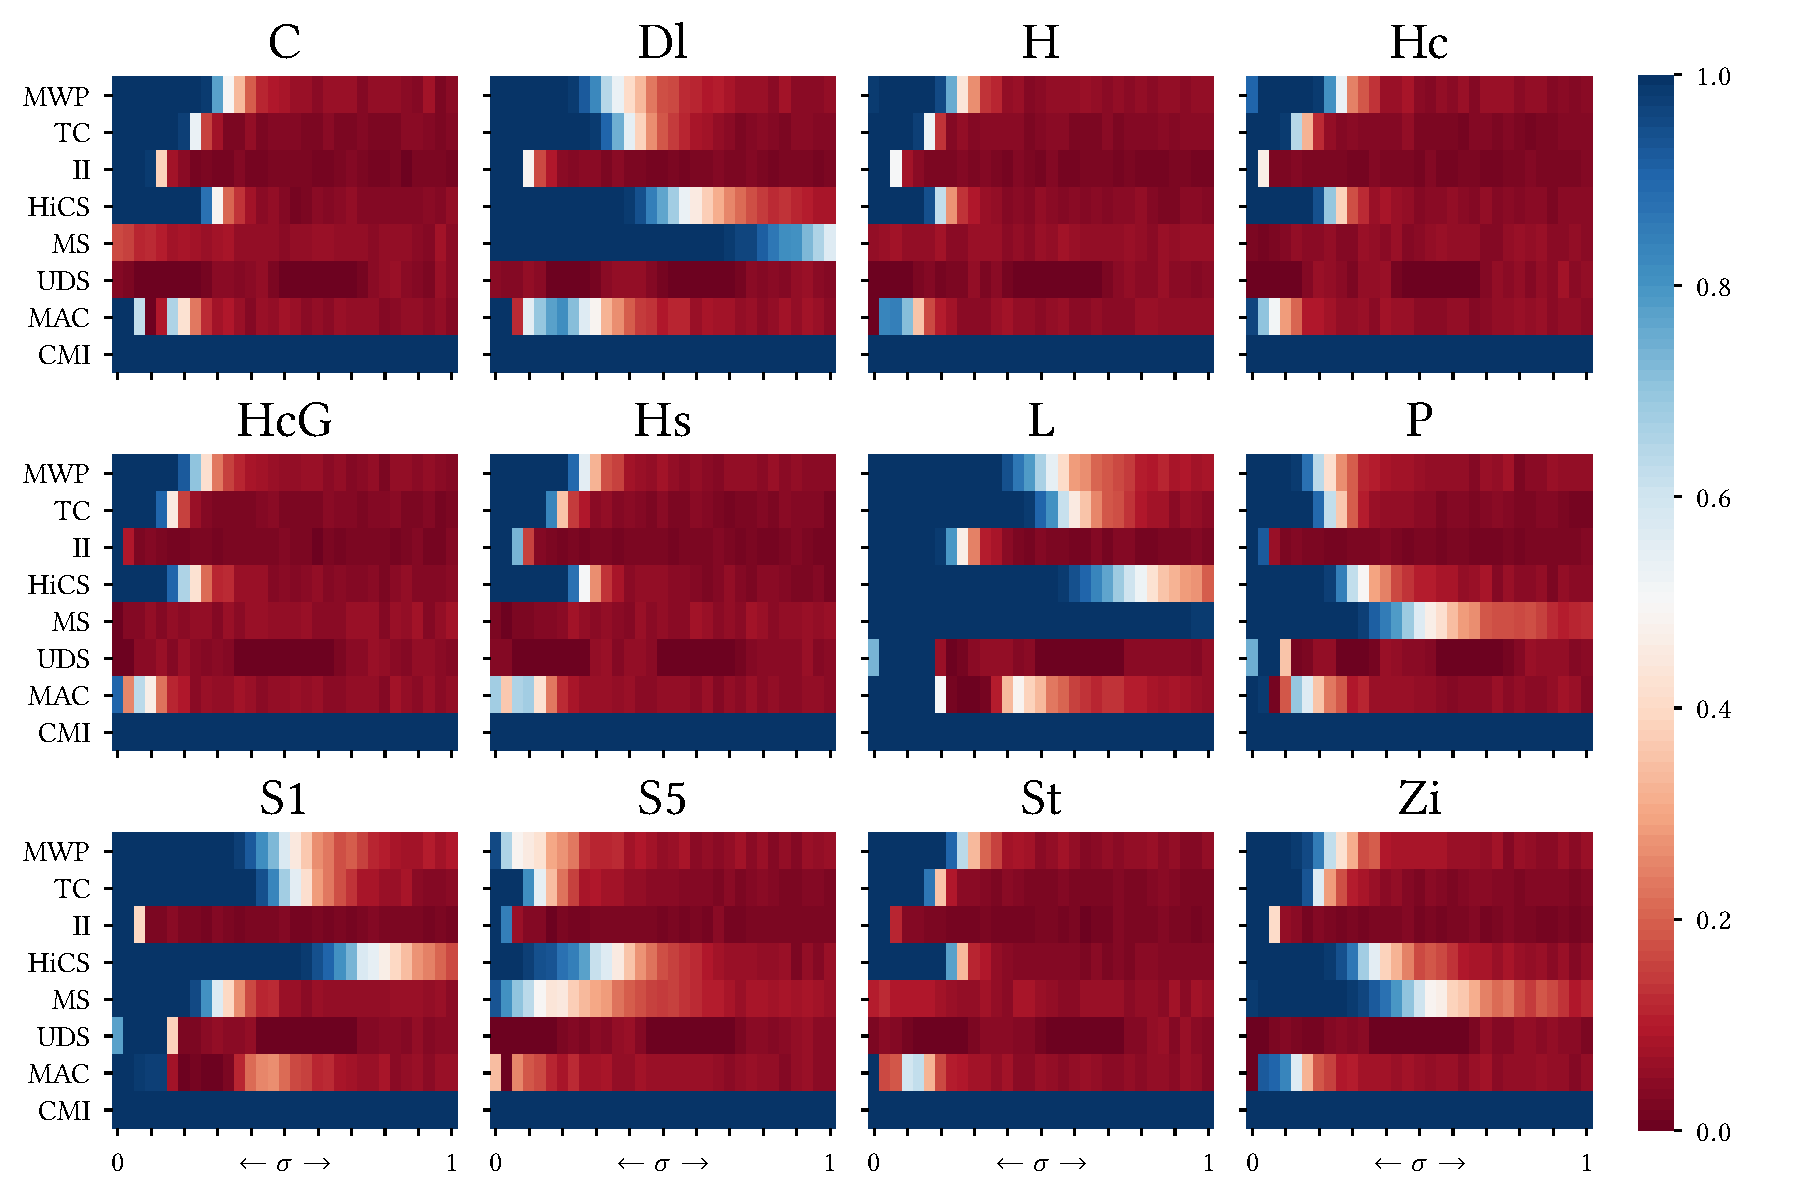
\includegraphics[width=1.0\linewidth]{part2-figures/Fig7_d3-2_thesis-compressed.pdf}}
\end{subfigure}
\begin{subfigure}[$|\gls{S}|=5$]
	{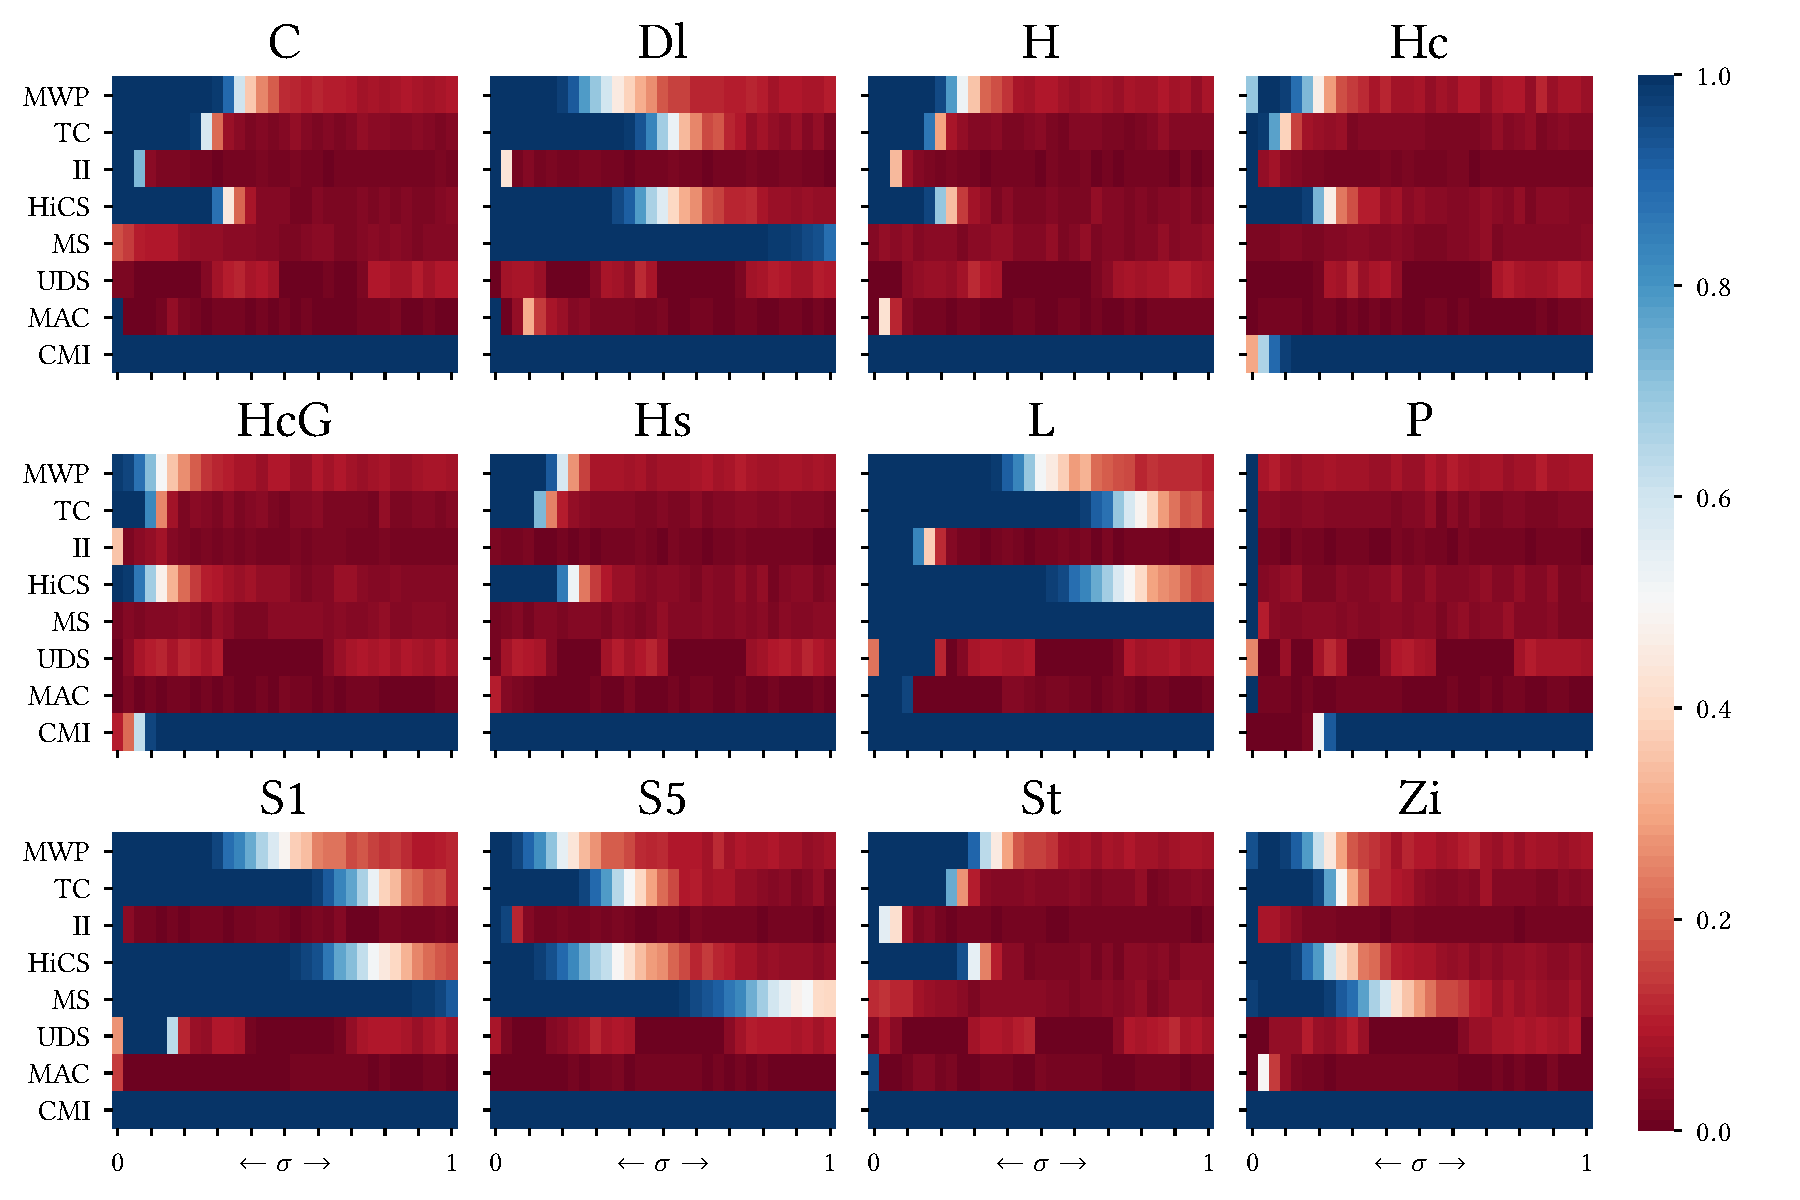
\includegraphics[width=1.0\linewidth]{part2-figures/Fig7_d5-2_thesis-compressed.pdf}}
\end{subfigure}
\caption{Power against each dependency.}
\label{fig:E_Power}
\end{figure}

Figure \ref{fig:E_Power} reveals that \gls{MWP}, \gls{TC} and \gls{HiCS} achieve high power in any situation up to a certain extent of noise. 
\gls{MWP} shows slightly more power with C, H, Hc, HcG, Hs and St.  
\gls{II} can detect almost every dependency, but the power decreases rapidly with noise and dimensionality. \gls{MS} detects Dl, L, P, S1, S5 and Zi, but misses all other dependencies. 
\gls{MAC} looks unstable since its power evolves in a non-monotonous way and decreases with increasing dimensionality by much. In fact, it is not able to detect most dependencies for $|\gls{S}|=5$.  
\gls{UDS} can only detect L, P and S1, a clear limitation. 
\gls{CMI} has maximal power for each dependency and noise level for $|\gls{S}|=3$, which is unrealistic: \gls{CMI} reaches its lowest score against the noiseless I, our baseline for power. This means that \gls{CMI} does not clearly distinguish noise from dependence. 

\subsubsection{Sensitivity}
\label{sensitivity}

\hyperlink{R6}{\textbf{R6}} states that estimators should reflect the strength of the observed effect w.r.t. the number of observations. Figure \ref{fig:All_sensitivity} graphs the average score from 500 instances of each dependency with a minimal noise of $1/30$. The average of \gls{MWP} obtained for each dependency converges to 1 consistently with more samples, except for I, which stabilises around $0.5$. This means that \gls{MWP} is sensitive (\hyperlink{R6}{\textbf{R6}}). 

\gls{TC} behaves similarly to \gls{MWP}. %: When the sample size increases, the score tends to increase as well. 
However, it is not bounded. While the scores of \gls{II} seem to increase with sample size, their absolute value decreases. %, except for \textbf{Hs}. 
\gls{MS} is %completely 
insensitive to changes in sample size. \gls{HiCS}, \gls{UDS}, \gls{MAC} and \gls{CMI} behave differently: their scores tend to go down as the sample size increases, even with I. This implies that their minimum or maximum score varies with the sample size, also highlighting interpretability (\hyperlink{R5}{\textbf{R5}})  problems. 

\begin{figure}
	\centering
	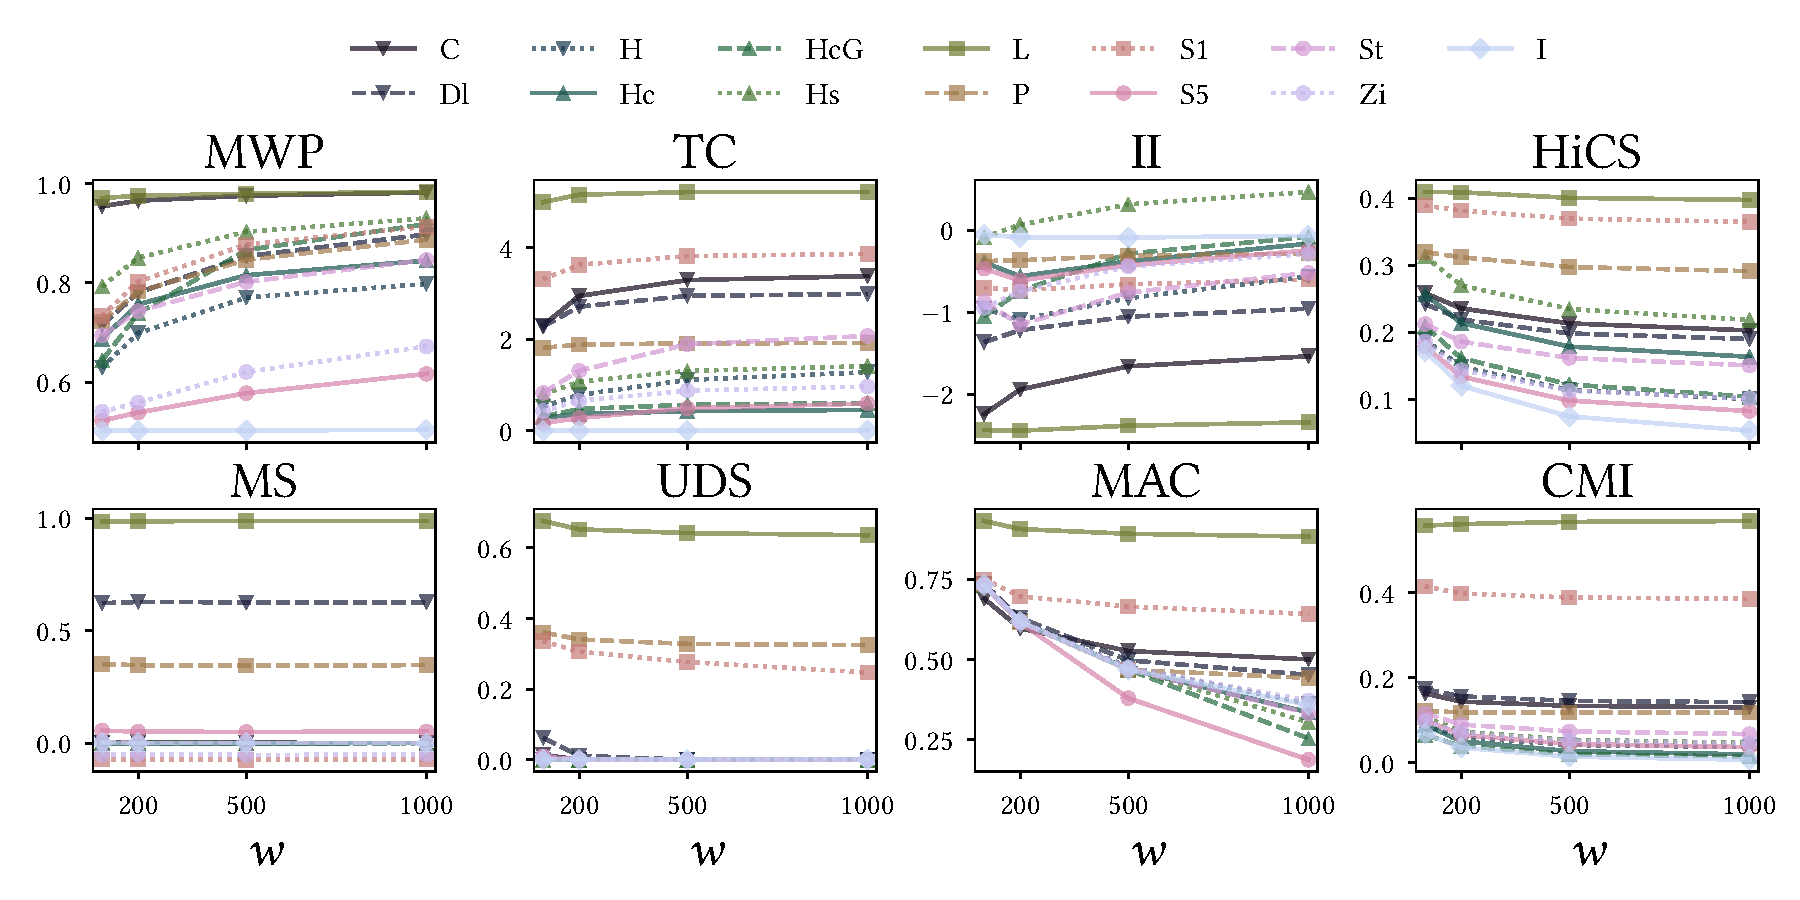
\includegraphics[width=\linewidth]{part2-figures/Fig8-2_thesis-compressed.pdf} 
	\caption{Average score w.r.t. $\gls{w}$, $\sigma = 1/30$.}
	\label{fig:All_sensitivity}
\end{figure} 

\subsubsection{Robustness}
\label{robustness}

\begin{figure}
	\centering
	\begin{subfigure}[Power]
		{\label{fig:E_Discrete_Power}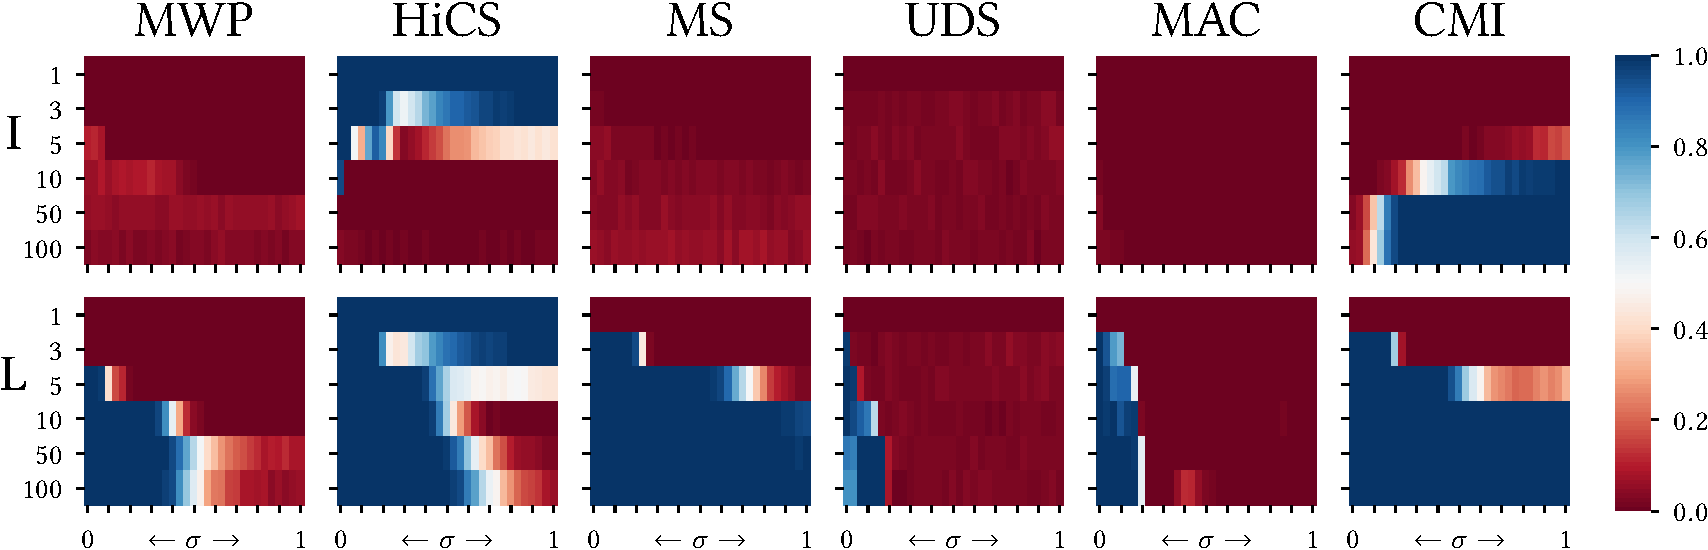
\includegraphics[width=\linewidth]{part2-figures/Fig9_1_thesis-crop-compressed.pdf} }
	\end{subfigure}
	\begin{subfigure}[Average]
		{\label{fig:E_Discrete_average}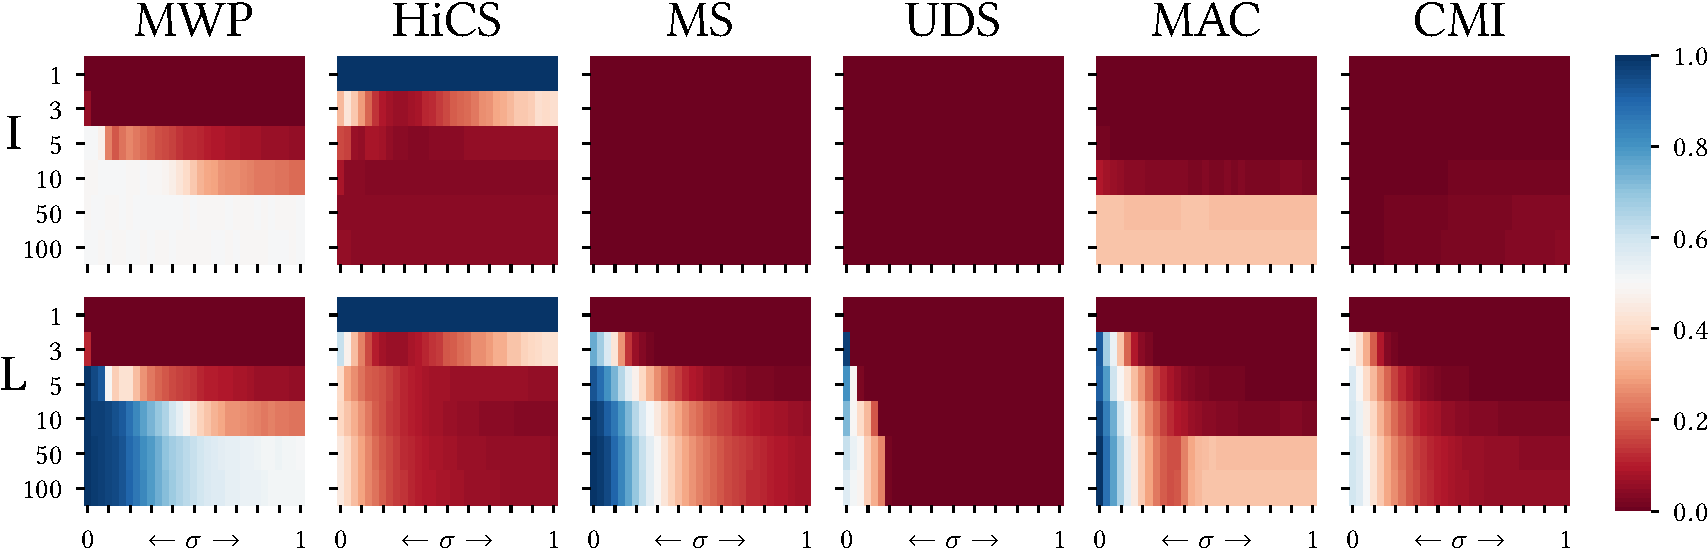
\includegraphics[width=\linewidth]{part2-figures/Fig9_2_thesis-crop-compressed.pdf}  }
	\end{subfigure}
	\caption{Power and average score w.r.t. $\omega$.}
	\label{fig:E_Discrete}
\end{figure} 

Data is often imperfect, i.e., values are rounded or trimmed. In some cases, this may lead to wrong estimates, e.g., an independent space is declared as strongly dependent. 

We simulate data imperfections by discretising a 3-dimensional linear dependency into a number $\omega$ of discrete values from 100 to 1. With only one value, the space is entirely redundant, i.e., its \textit{contrast} should be minimal. We compare the power of \gls{MWP} and the other approaches against L and I for different levels of discretisation. Since \gls{TC} and \gls{II} base on local neighbourhoods, they do not work in this setting%they fail when the same observation is present more than $k$ times, i.e., they are by design not robust
; We exclude them from the analysis. Figure \ref{fig:E_Discrete_Power} displays the results.

\gls{HiCS} yields high power in the case of discrete values, even for I. %This is because \gls{HiCS} uses the \textit{Kolmogorov-Smirnov} test which assumes continuous data. 
Thus, \gls{HiCS} is not robust. Also, the power of \gls{CMI} wrongly increases as we add noise to I, provided that $\omega \geq 10$. 
This is why the power of \gls{CMI} is high for every dependency in Figure \ref{fig:E_Power}. \gls{CMI} rejects the independence for independent spaces, i.e., it is not robust. On the other hand, \gls{MWP}, \gls{MS}, \gls{UDS} and \gls{MAC} seem robust (\hyperlink{R7}{\textbf{R7}}).

In Figure \ref{fig:E_Discrete_average}, we see that the score of \gls{CMI} tends to increase slightly for I as we add noise, whenever $\omega > 5$. Also, the score of \gls{HiCS} increases for both I and L when $\omega \leq 5$. \gls{MAC} converges to $0.4$ as noise increases for $\omega > 10$. On the other hand, \gls{MWP} converges to $0$ as the space becomes discrete. This is an interesting feature of our estimator: discrete spaces are of lower interest since the notion of \textit{contrast} is not clearly defined there. It allows analysts to draw a line between discrete and real-valued attributes, characterizing their relevance for further analysis.   

\subsubsection{Scalability}
\label{sec:scalability}

\begin{figure}
	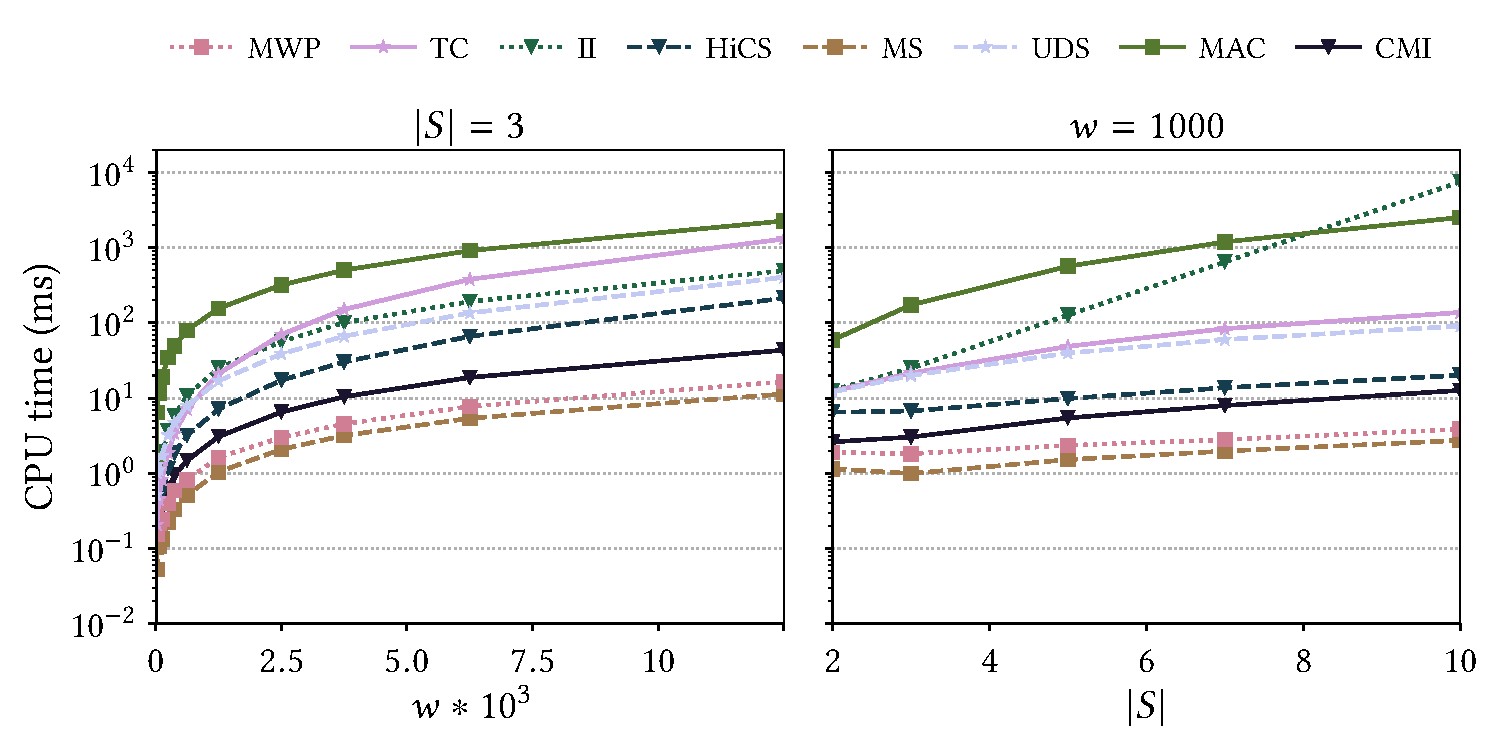
\includegraphics[width=1.0\linewidth]{part2-figures/Fig10-2_thesis-compressed.pdf} 
	\caption{Execution time w.r.t. $\gls{w}$ and $|\gls{S}|$.}
	\label{fig:Runtime_n_d}
\end{figure} 

We now look at the runtime requirements of our approach. We measure the average time for each estimator against $500$ independent data sets with growing $\gls{w}$ and $|\gls{S}|$. Note that which data set we use only has a marginal effect on the measured time. For consistency, we use instantiations of I for every estimator. 
Figure \ref{fig:Runtime_n_d} graphs the results. As we can see, \gls{MWP} is the second fastest after \gls{MS}. 
\gls{HiCS} and \gls{CMI} scale relatively well with $\gls{w}$ and $|\gls{S}|$. There is a second group formed by \gls{TC}, \gls{II} and \gls{UDS} one order of magnitude slower. However, \gls{II} does not scale well with $|\gls{S}|$. \gls{MAC} is way behind all others. One should note that the runtime of \gls{MWP} can be further improved via parallelisation and prior indexing.

We evaluate the scalability of index construction for each approach, by increasing the size of the sliding window $\gls{w}$ from $10^2$ to $10^5$ in an independent space I with three dimensions. 
The red line (`Construction') is the average time for creating the index with window size $\gls{w}$ (Algorithms \ref{indexconstruction}/\ref{kspconstructindex}/\ref{cspconstructindex}). 
The other lines show the average time to insert a new point into the window.   
\begin{figure}
    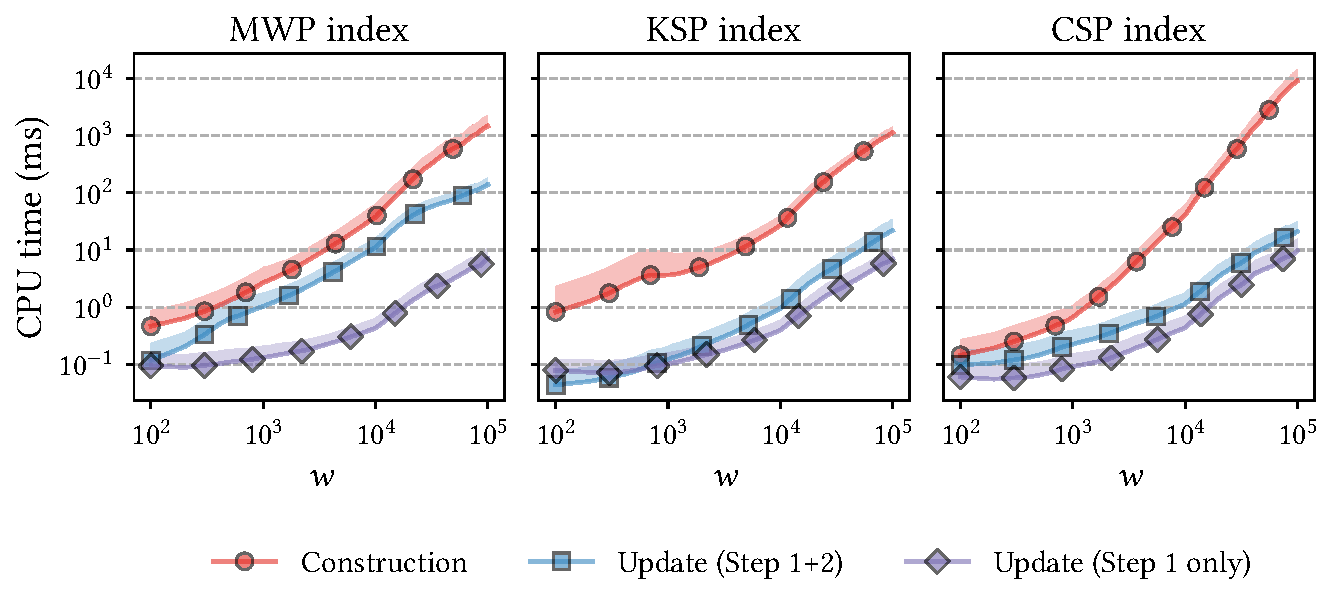
\includegraphics[width=\linewidth]{part2-figures/indexperformance_thesis-compressed.pdf}
    \caption{Time required for index construction and update w.r.t. window size $\gls{w}$.}
    \label{fig:scalability-index}
\end{figure}

In Figure \ref{fig:scalability-index}, we can see that the construction time of each index increases almost linearly with increasing window size $\gls{w}$. 
The \gls{KSP} index is less expensive to update than \gls{MWP}, regarding \textsc{Step 2} in particular. 
The first step of the \gls{CSP} index update is very efficient, as it requires more or less constant time (see Table \ref{tab:complexity}). 
We can see that only performing \textsc{Step 1} in our update operations, while delaying \textsc{Step 2} to the contrast estimation step, reduces the execution time by up to 3 orders of magnitude, compared to standard index construction. 
So we can significantly speed up the monitoring of \gls{MCDE} contrast using the index update operations. 

In Figure \ref{fig:scalability-contrast}, we compare the execution time estimating \gls{MWP}, \gls{KSP}, and \gls{CSP}, with increasing window size $\gls{w}$. 
We can see that the three approaches have a comparable execution time. 
\gls{KSP} is slightly slower for small window sizes because the $\overline{p}$-values are more difficult to obtain than with the other approaches. 
However, as the window size increases, \gls{KSP} and \gls{MWP} have the same execution time. 
\gls{CSP} contrast estimation appears to be slightly slower as the window size increases but scales similarly. 

\begin{figure}
    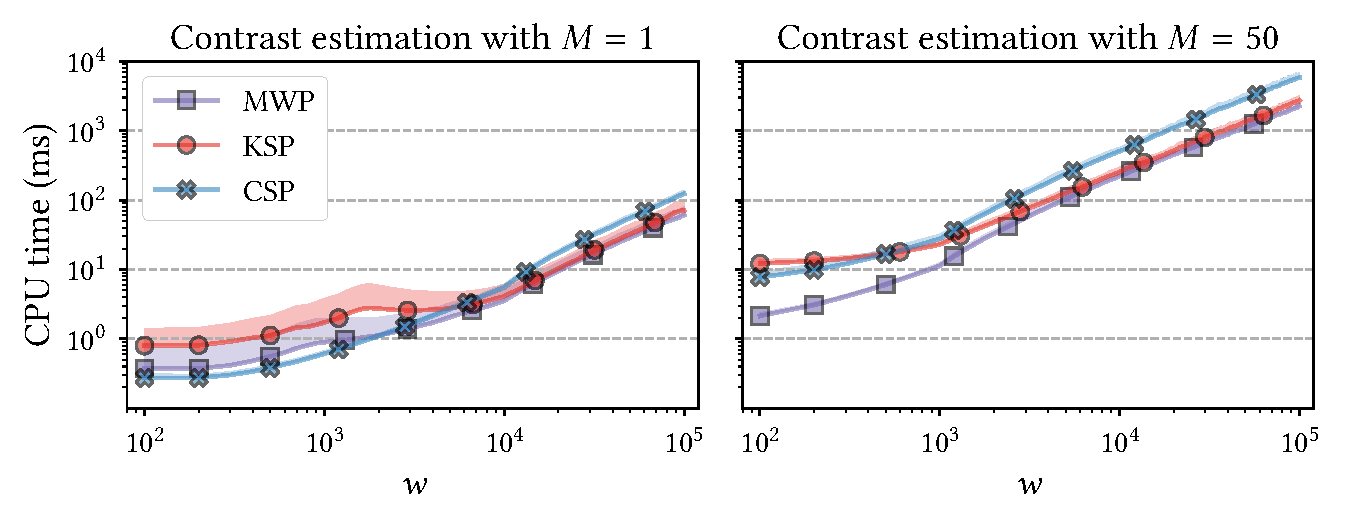
\includegraphics[width=\linewidth]{part2-figures/contrastperformance_thesis-compressed.pdf}
    \caption{Time required for contrast estimation w.r.t. window size $\gls{w}$.}
    \label{fig:scalability-contrast}
\end{figure} 

\subsubsection{Deployment to the Streaming Setting}

We monitor contrast when the dependency gradually evolves. 
We simulate this setting by concatenating $100$ three-dimensional linear dependencies with $1\,000$ observations each and a level of noise $\sigma$ 
linearly increasing from $0$ to $1$. 
We use the approach described in Section \ref{adaptation-stream}, Equation \ref{eq:exp-decay} and instantiate \gls{MCDE} with \gls{MWP}. We estimate the dependency over a sliding window of size  $w=1\,000$ and with a decaying factor $\gamma = 0.99$. 

We let $\Delta$ vary from $1$ to $1\,000$ and $M$ from $1$ to $500$. 
We compare each configuration to a baseline, which is the most expensive configuration ($\Delta=1$, $M=500$), without the benefit of our update operations. 
When $\Delta > 1$, we simply set the current contrast estimate to the value from the latest estimation. We define the following measures: 
\begin{itemize}[noitemsep]
    \item The \textbf{Absolute Error} is the average absolute difference between the values obtained with the tested configuration and the values from the baseline. 
    \item The \textbf{Relative Time} is the ratio of the time required by the tested con\-fi\-gu\-ra\-tion over the time required by the baseline.
    \item The \textbf{Index Speedup} is the ratio between the time required by the tested configuration without/with our index update operations.  
\end{itemize}

We can see from Figure \ref{fig:stream-experiment} that the absolute error decreases with $\Delta$, while the relative execution time increases. 
The speedup obtained by our index operations is responsible for this gain in efficiency to a large part. 
As we increase the number of iterations $M$, the errors tend to decrease, but at the same time, contrast estimation dominates the overall execution time. 
In such cases, we see less benefit from our efficient insert/delete operations. 

We identify the configuration $M=50$, $\Delta=50$ as a sweet spot: for an absolute error as small as $\approx0.01$, the computational burden is reduced by up to $100$ times, with a consistent index speedup of $3$. We mark this configuration with a star $*$ in the figure. 
 
\begin{figure}
	\centering
    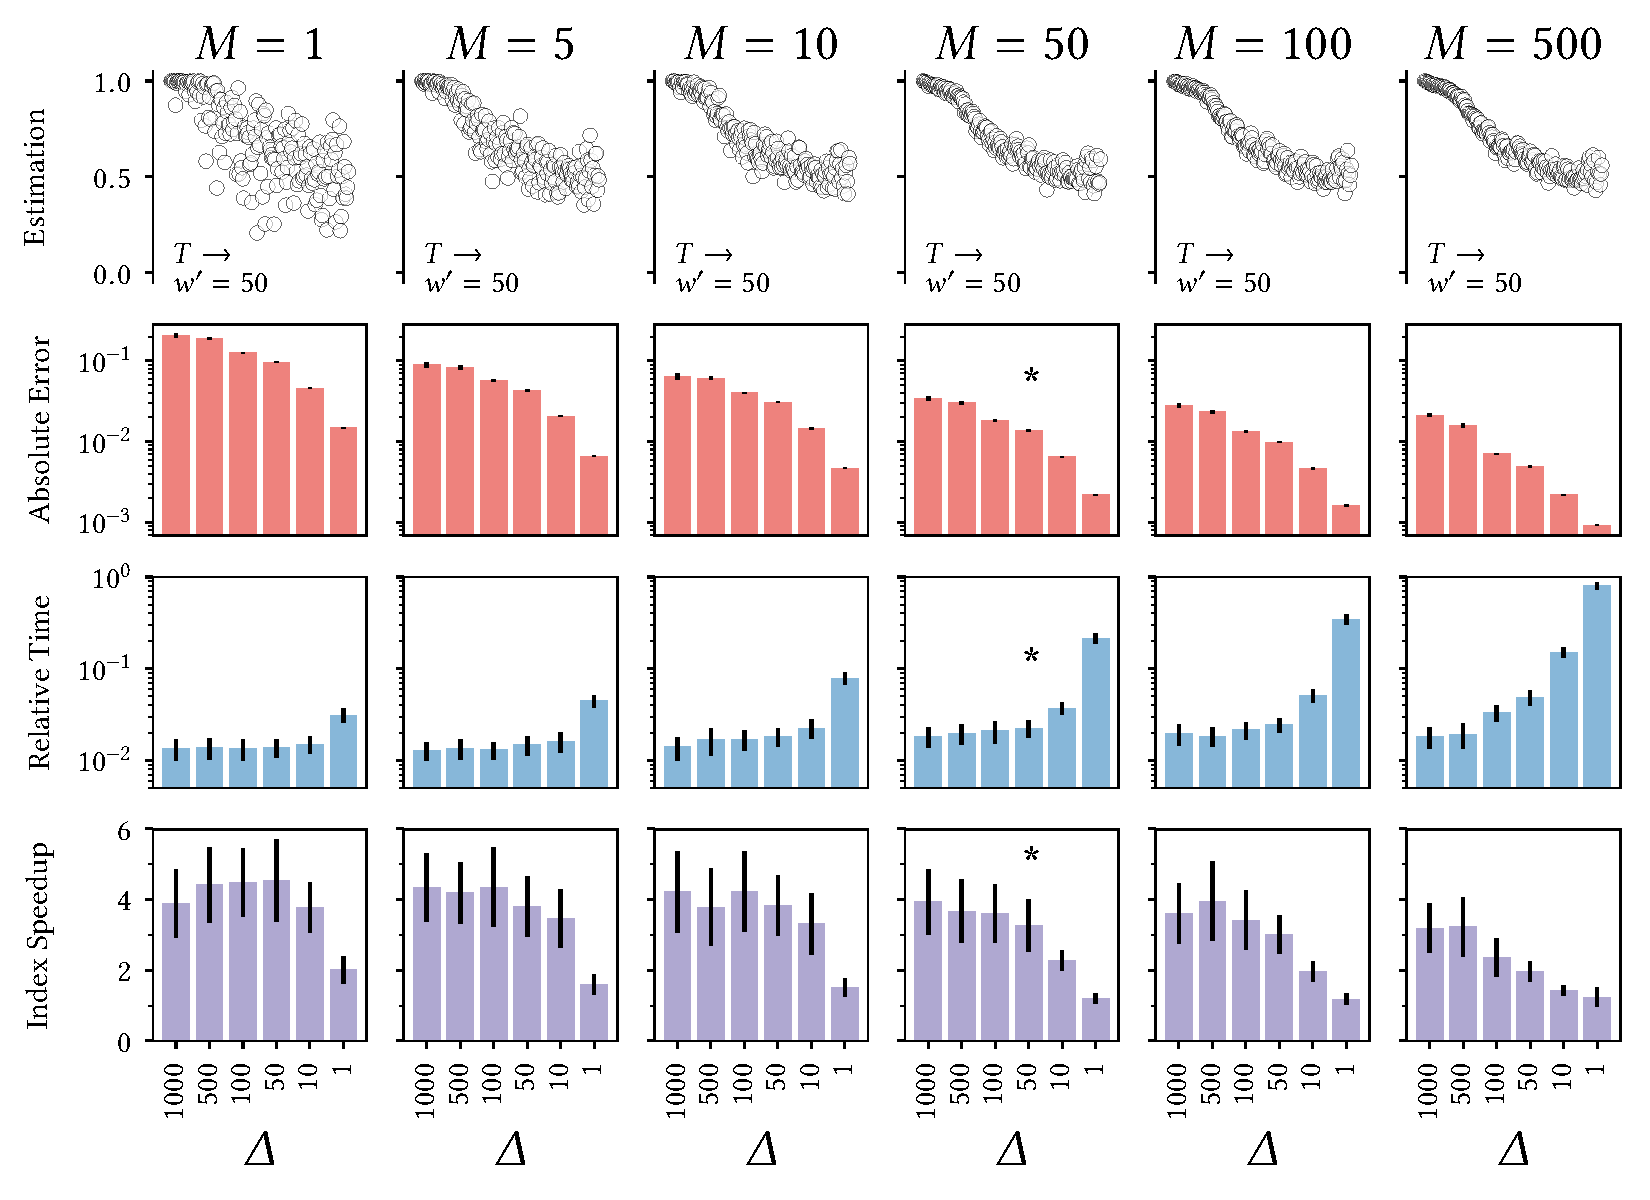
\includegraphics[width=\linewidth]{part2-figures/all_thesis-compressed.pdf}
    \caption{Performance of contrast estimation with \textit{concept drift} (* $\equiv$ sweet spot).}
    \label{fig:stream-experiment} 
\end{figure} 

\subsection{Case Study: Discovering Dependency Patterns}

\glsunset{Bioliq}
We now apply \gls{MCDE} to a real-world multivariate time series. 
The data was collected during a 4-day production campaign at \gls{Bioliq}, a pyrolysis plant in the surroundings of Karlsruhe  \cite{pfitzer2016fast}. It contains one measurement per second, i.e., $345\,600$ observations, from a selection of 20 physical sensors %, such as temperature or pressure, 
in various components of the plant. 
We monitored the evolution of dependency between each sensor pair with $\gls{w} = 1000,  \Delta = 50$, $M=50$, as just explained. 
We obtained the evolution of dependency between the $20$ sensors (i.e., $190$ pairs) using a single CPU core in about $2$ hours. Note that it would be easy to shorten the computation time significantly by parallel processing.  

We have presented the results of our monitoring technique to the plant operators. 
They have identified several patterns which they deemed `interesting', i.e., patterns yielding insights that could help with plant operation. 

Figure \ref{fig:real-world-pattern} displays one of these patterns. 
It is the result of monitoring two sensors, namely the pressure at the reactor input, and the oxygen concentration at the output. 
As we see, the dependency between these two measures changes significantly over time. 
Some changes, marked in the figure from 1 to 4, appear to represent different stages in the production process. 
A better understanding of the dynamics of the physical measures involved in the reaction will help the plant owners to operate smoothly and efficiently. 

\begin{figure}
\centering
    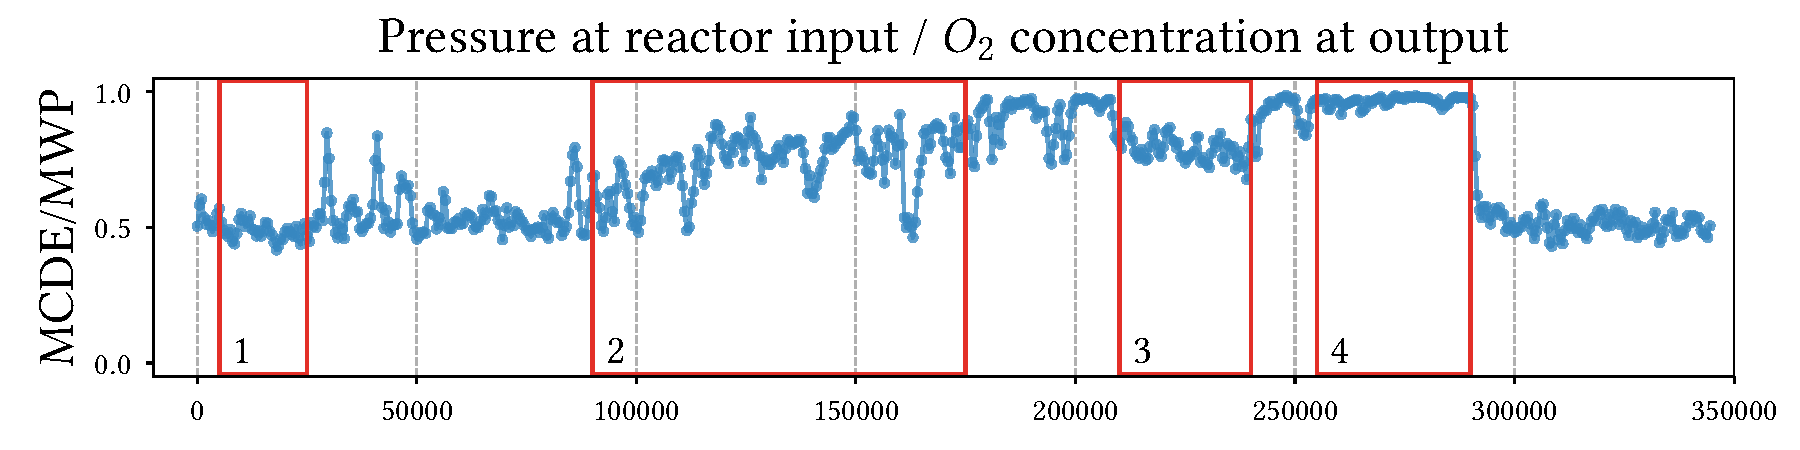
\includegraphics[width=1\linewidth]{part2-figures/Dep_example_thesis-compressed.pdf}
    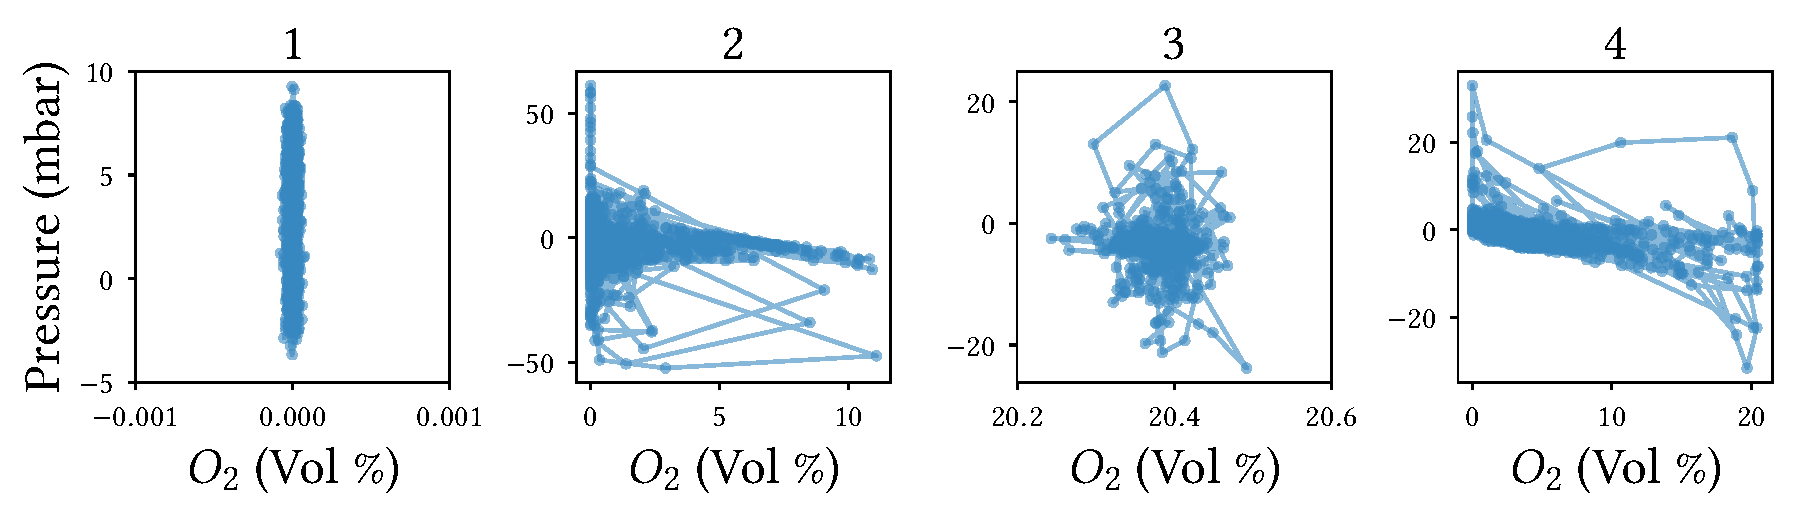
\includegraphics[width=1\linewidth]{part2-figures/Dep_example_details_thesis-compressed.pdf}
    \caption{Example of an interesting dependency pattern in the pyrolysis data.}
    \label{fig:real-world-pattern}
\end{figure}

\section{Discussion}

Our experiments show that \gls{MCDE} fulfils all requirements linked to heterogeneous data streams and has the desirable features of a framework for dependency estimation. %Each MCDE instantiations (MWP, KSP and CSP) are state of the art dependency estimators, which we can combine to tackle the challenging H-DS setting. 

First, we can see that \gls{MCDE} is efficient (\hyperlink{C1}{\textbf{C1}}), and, thanks to the index update operations, one can use it in combination with the sliding window model to mine data streams in a single scan (\hyperlink{C2}{\textbf{C2}}) and adapt (\hyperlink{C3}{\textbf{C3}}) the contrast estimation over time, taking \textit{concept drift} into account. 
Second, one can also reduce or increase the number of MC iterations $M$ to trade between accuracy and computation time, in an anytime (\hyperlink{C4}{\textbf{C4}}) fashion. \gls{MCDE} can handle heterogeneity (\hyperlink{C5}{\textbf{C5}})  via the instantiation of various statistical tests.

Each approach, except \gls{MCDE} and \gls{MS}, has at least one unintuitive parameter (\hyperlink{R3}{\textbf{R3}}): \gls{TC} and \gls{II} require $k \in \mathbb{N}$, \gls{CMI} requires $Q \in \mathbb{N}$, \gls{MAC} requires $\epsilon \in (0,1)$, \gls{UDS} requires $\beta \in \mathbb{N}$, \gls{HiCS} requires $\alpha \in (0,1)$. Next, only \gls{MCDE} and \gls{HiCS} allow trading accuracy for a computational advantage (\hyperlink{C4}{\textbf{C4}}). Note that, by adapting recent anytime estimators for \gls{MI} such as \cite{DBLP:conf/edbt/VollmerB19}, \gls{TC} and \gls{II} maybe potentially also fulfil \hyperlink{C4}{\textbf{C4}}. 

Last, \gls{MCDE} is non-parametric (\hyperlink{R4}{\textbf{R4}}) and interpretable (\hyperlink{R5}{\textbf{R5}}) by design. 
Our experiments against an assortment of dependencies show that it is multivariate (\hyperlink{R1}{\textbf{R1}}), general-purpose (\hyperlink{R2}{\textbf{R2}}) and robust (\hyperlink{R7}{\textbf{R7}}). \gls{MCDE} is sensitive (\hyperlink{R6}{\textbf{R6}}) because estimates are the average of $\overline{p}$-values. Table~\ref{table:requirements} summarises our findings.

\begin{table}[ht]
	\caption{Fulfilment of Constraints and Requirements.} 
	%\footnotesize
	\centering
	\small
	\setlength\extrarowheight{-4pt}
	\begin{tabular}{l | c c c c c | c c c c c c c} 
		\toprule 
		Estimator 		&\hyperlink{C1}{\textbf{C1}}	& \hyperref[C2]{\textbf{C2}} 	& \hyperlink{C3}{\textbf{C3}} &\hyperref[C4]{\textbf{C4}} &\hyperref[C5]{\textbf{C5}}	& \hyperlink{R1}{\textbf{R1}}	& \hyperlink{R2}{\textbf{R2}}  & \hyperlink{R3}{\textbf{R3}}	& \hyperlink{R4}{\textbf{R4}}	& \hyperlink{R5}{\textbf{R5}} 	& \hyperlink{R6}{\textbf{R6}}	& \hyperlink{R7}{\textbf{R7}} \\ 
		\midrule 
		\gls{MS} 	& ++ 			& \xmark 		& \xmark	& \xmark & \xmark 		& \cmark      	& \xmark 		& \cmark 	& \cmark 		& \cmark 		& \xmark		& \cmark \\ 
		\gls{TC} 	& -				& \cmark 		& \cmark 	& \cmark & \xmark 		& \cmark 		& \cmark 		& \xmark 	& \cmark 		& \xmark 		& \cmark		& \xmark \\
		\gls{II} 	& -{}- 			& \cmark 		& \cmark 	& \cmark & \xmark 		& \cmark 		& \xmark 		& \xmark 	& \cmark 		& \xmark 		& \xmark 		& \xmark \\
		\gls{CMI} 	& + 			& \xmark 		& \xmark 	& \xmark & \xmark 		& \cmark 		& \xmark 		& \xmark 	& \cmark 		& \xmark 		& \xmark		& \xmark \\
		\gls{MAC} 	& -{}- 			& \xmark 		& \xmark 	& \xmark & \xmark 		& \cmark 		& \xmark 		& \xmark 	& \cmark 		& \xmark 	 	& \xmark		& \cmark \\
		\gls{UDS} 	& - 			& \xmark 		& \xmark 	& \xmark & \xmark		& \cmark 		& \xmark  		& \xmark 	& \cmark 		& \xmark 		& \xmark		& \cmark \\ 
		\gls{HiCS} 	& +				& \xmark 		& \xmark 	& \cmark & \xmark		& \cmark 		& \cmark 		&  \xmark 	& \cmark 		& \xmark 		& \xmark		& \xmark \\ 
		\gls{MCDE} 	& ++ 			& \cmark 		& \cmark	& \cmark & \cmark		& \cmark 		& \cmark 		& \cmark 	& \cmark 		& \cmark 		& \cmark		& \cmark \\
		\bottomrule
	\end{tabular}
	\label{table:requirements}
\end{table}
 
All in all, \gls{MCDE} yields to state-of-the-art estimators: it is versatile, allowing quality-runtime trade-offs and parallelisation, which is useful when time is critical, e.g., in large data streams. At the same time, it shows excellent detection quality with no restriction on the dependency type, while being easy to use and interpret. \gls{MCDE} features a blend of properties that so far no competitor offers. 

In this chapter, we have described a framework to estimate multivariate dependency in heterogeneous data streams. 
It fulfils all requirements one would expect from a state-of-the-art dependency estimator. 
Compared to other approaches, it provides high statistical power on a large panel of dependencies, while being very efficient. Furthermore, we introduced index operations for the streaming setting and illustrated the benefits of our framework against a real-world use case. In the next part, we generalise the task of dependency estimation to monitoring large sets of statistics. 